%\documentclass[UTF8]{ctexart}
\documentclass[11pt]{article}
\usepackage{geometry}
\geometry{left=3.18cm,right=3.18cm,top=2.54cm,bottom=2.54cm}
\usepackage{graphicx}
\usepackage{subfig}
\usepackage{float}
\pagestyle{plain}    
\usepackage{setspace}
\usepackage{array}
\usepackage{booktabs} %调整表格线与上下内容的间隔
\usepackage{indentfirst} % 首行缩进
\usepackage{fancyhdr}
\usepackage{fancybox}
\usepackage{enumitem}
\usepackage{amsmath}
\usepackage{xeCJK}
\setCJKfamilyfont{song}{SimSun}
\setCJKfamilyfont{hei}{SimHei}
\setCJKfamilyfont{xingkai}{STXingkai}
\setCJKfamilyfont{kai}{KaiTi}
\setCJKfamilyfont{fang}{FangSong}
\newcommand{\song}{\CJKfamily{song}}
\newcommand{\hei}{\CJKfamily{hei}}
\newcommand{\kai}{\CJKfamily{kai}}
\newcommand{\fang}{\CJKfamily{fang}}
\setlength{\parindent}{2em}
\newcommand{\upcite}[1]{\textsuperscript{\textsuperscript{\cite{#1}}}}
\renewcommand{\refname}{}
\renewcommand{\figurename}{图}
\begin{document}
\pagestyle{empty}
\thispagestyle{empty}
\begin{flushleft}
\fontsize{12.0pt}{\baselineskip} \selectfont 附件1
\end{flushleft}
\vskip 10pt
\begin{center}
\quad \\
\setlength{\baselineskip}{40pt}{\hei \fontsize{28pt}{10pt} \selectfont 中 \hspace{0.1em} 南 \hspace{0.1em} 大 \hspace{0.1em} 学\\研究生学位论文开题报告}
\end{center}
\vskip 150pt
\begin{center}
\begin{tabular}{l}
\fontsize{12pt}{10pt} \selectfont
姓 \ \ \ \qquad 名:\underline{\hspace{7em}王向宇\hspace{7em}}\\

\specialrule{0em}{5pt}{5pt}

\fontsize{12pt}{10pt} \selectfont
学 \ \ \ \qquad 号:\underline{\hspace{6.3em}195001029\hspace{6.3em}}\\

\specialrule{0em}{5pt}{5pt}

\fontsize{12pt}{10pt} \selectfont
论 \ 文 \ 题 \ 目:\underline{\hspace{1.5em}基于深度学习的地震成像新算法\hspace{1.5em}}\\

\specialrule{0em}{5pt}{5pt}

\fontsize{12pt}{10pt} \selectfont
攻 \ 读 \ 学 \ 位: \underline{\hspace{7.5em}博士\hspace{7.5em}}\\

\specialrule{0em}{5pt}{5pt}

\fontsize{12pt}{10pt} \selectfont
指 \ 导 \ 教 \ 师: \underline{\hspace{7em}冯德山\hspace{7em}}\\

\specialrule{0em}{5pt}{5pt}

\fontsize{12pt}{10pt} \selectfont
学 \ 科 \ 专 \ 业: \underline{\hspace{4em}地球探测与信息技术\hspace{4em}}\\

\specialrule{0em}{5pt}{5pt}

\fontsize{12pt}{10pt} \selectfont
二 \ 级 \ 单 \ 位: \underline{\hspace{3em}地球科学与信息物理学院\hspace{3em}}\\

\specialrule{0em}{5pt}{5pt}

\fontsize{12pt}{10pt} \selectfont
填 \ 表 \ 日 \ 期: \underline{\hspace{4.3em}2020年11月15日\hspace{4.3em}}\\
\end{tabular}
\end{center}

\begin{center}
\vskip 100pt
\hei \fontsize{14pt}{10pt} \selectfont 中南大学研究生院制
\end{center}
\newpage

\fancypage{
\setlength{\fboxsep}{0.5pt}
\setlength{\fboxrule}{0.5pt}
\setlength{\shadowsize}{0pt}
\shadowbox}{}
\setlength{\baselineskip}{15pt}
\section*{\hei\fontsize{11pt}{10pt} \selectfont \\ 一、选题意义和研究价值}
\subsection*{\kai\fontsize{11pt}{10pt} \selectfont【选题意义】}
随着全球经济的快速发展和科学技术水平的逐渐进步,石油资源已经成为支撑各个行业发展的基础能源。世界各国也越来越重视油气资源的勘探问题。随着中国经济的蓬勃发展,对于能源的消耗也日益加大,因此,油气资源短缺的问题也日益突出,然而油气资源的形成需要古生物经过漫长的时间演化而来,属于典型的非可再生能源,按照全国油气资源评价和探明储量通报,我国油气资源丰富,但资源探明程度不高,主要是由于油气储层的地质构造十分复杂,为油气勘探带来了巨大的困难,鉴于这个原因,发展高精度的地震勘探技术也逐渐成为科研工作者研究的重点。随着数学、物理理论的逐步提升和计算机硬件水平的快速更新,地震勘探的水平也随之提高,油气的探明率和开采率都得到了巨大的提升。地震波的数值模拟是许多地震处理程序的组成部分,地震勘探的主要问题涉及偏移成像、地震剖面数据处理、反演成像等。
\par
地震勘探可以分为三个环节:地震资料野外采集、地震资料数据处理、以及资料解释。其中地震信号处理的重要目标是提高信号质量。随着地震勘探技术的提高,油气、煤炭的勘探目标逐渐向地质条件更复杂的山区、林地和沙漠地区转移。复杂的地质结构和开采环境导致地震勘探数据中反射同相轴形态复杂,信号能量弱,同时地震勘探数据中还伴随着大量的噪声,这种低信噪比地震勘探数据给有效信息的识别带来困难,在强噪声区域甚至掩盖了有效信号。进而影响了对地下构造信息的解释。因此,压制地震勘探噪声,提高地震勘探数据质量,是地震勘探信号处理的重要且基础性工作。压制地震勘探数据中的随机噪声能够有效提高地震勘探数据质量。按产生源头可以将地震勘探随机噪声分为两类:自然噪声和人文噪声。自然噪声指自然力
量作为噪声源产生的随机干扰,比如风吹动时对地面的作用,以及对草、农作物、树木吹动时造成的振动,由风造成的噪声统称为风噪声。如果采样点在水边,海浪的拍打,河流的流动,也都会使数据中引入自然噪声。人文噪声指人类的活动引起的噪声,分为近场人文噪声和远场人文噪声两类。近场人文噪声主要是人员引起的噪声,比如人走动,机器运转造成的噪声。这部分噪声采用伪谐波函数进行拟合。远场人文噪声指远方的人类活动造成的干扰,比如交通、工厂的生产等。考虑这种造声来自各个方位,噪声源是随机的,所以,通常认为地震勘探数据中随机噪声的产生为平稳随机过程。这些噪声导致地震信号的信噪比降低。为此,我们需要对地震数据进行去随机噪声处理,以获得具有高信噪比记录,为后续处理打下基础。
\par
地震偏移成像是地震勘探数据处理的重要技术手段。地震勘探技术的成败很大程度上决定于偏移技术,偏移是获取地下波阻抗界面几何构造形态行之有效的方法之一;在一定程度上,可以认为偏移技术的好坏就代表了地震勘探技术的好坏。本质上说地震偏移是利用数学方法使观测到的数据反向(逆时)传播,从中去除地震波传播过程的效应,最终得到勘探区地下结构的过程。基于射线法,积分法,以及波动方程法所衍生的偏移方法种类繁多。基于波动方程法的逆时偏移是目前众多偏移方法中最受欢迎的方法之一,对比其他传统的偏移方法,逆时偏移需要更多的存储空间和更大的计算量,但是当前计算机的计算效率和存储空间已经非常的优越,足以满足逆时偏移的需求。逆时偏移的优势十分明显,在波场计算过程中既包含了地震波的动力学和运动学信息,可以对多种波成像。目前工业界存在多种成像条件,常见的成像条件有互相关成像条件和反褶积成像条件,互相关成像条件由于更加稳定,在工业界得到广泛应用。但是理论分析表明互相关成像条件是线性Born近似正演算子的共轭转置,而不是正演算子的逆,另外由于波场带宽有限、地下照明不均匀等因素的影响,常规的互相关成像条件只能对地下构造进行模糊成像,仅提供准确的地下构造信息。成像的分辨率较差,不能满足高精度地震成像的要求。
\par
地震反演是地震勘探的根本问题,其目的是提取地震波所蕴含的地下岩层速度结构和物性参数空间分布信息,为地质结构与资源勘探开发提供重要依据。全波形反演作为一种有效的从波动方程中反演物性参数的方法,具有高度非线性的特征。若初始模型与真实模型偏差过大,计算波场与观测波场相位差大于半个周期,会产生``周波跳跃''现象,导致反演陷入局部极小值而无法得到准确结果。因此如何为全波形反演提供一个良好的初始模型是关键问题。前人发展了很多速度建模方法,如偏移速度分析、叠加速度分析以及速度层析成像等方法均可以建立较为准确的初始速度模型,并能在一定程度上避免全波形反演过程中的局部极小和``周波跳跃''问题,但在反演中仍存在计算量大的不足。由于地震数据中,不同频率数据对应的周期不同,相比于低频数据,高频数据频率更高、周期更短,在进行计算波场与观测波场匹配时更容易出现``周波跳跃''现象,因此多尺度全波形反演成为一种可行方法。另一方面,地震全波形反演问题在数学上是不适定的,需要一些正则化方法获得稳定解。以Tikhonov正则化为代表的正则化理论是求解病态问题的重要技术方法,但得到的解过于平滑,不能反映边界信息。因此,如何合理地利用正则化理论与方法对地球物理中的反问题进行求解,从而得到具有地质地球物理意义的参数,仍是值得关注的研究课题。
\par
\newpage
\subsection*{\kai\fontsize{11pt}{10pt} \selectfont【研究价值】}
面对地震高精度成像的要求,开展基于深度学习的地震成像新算法,其研究价值如下:
\par
1) 基于深度卷积去噪自动编码器(Convolutional Denoising Autoencoders, CDAEs)的地震剖面去噪;
\par
由于在实际的地震探测过程中,地下介质复杂多变,存在各种人为设施的杂乱回波以及仪器本身或系统噪声等多种因素的影响,使得地震剖面中含有各种各样的杂波和噪声,降低了地震信号的质量。因此,研究高信噪比的保真地震数据去噪方法显得尤为重要。实际噪声在实践中是不可避免的,必须在预处理数据的同时对噪声处理。对地震数据进行去噪已经得到了广泛地研究,常用的方法有Fourier变换、Wavelet变换、Curvelet变换等。上述基于稀疏表示的去噪方法都有自己的优势,也有自己的局限性。其中最主要共同点是变换基固定,不能根据各种信号的特征而进行自我调整,然而地震剖面是比较复杂的信号数据,波形变化大,且由多种直线曲线元素构成,因此常规稀疏表示方法对于信号的准确表示有所不足。我们需要一种能够根据不同的地震资料自身的特点,设计一种能够适应地震剖面的去噪方法。CDAEs通过对模拟数据的不断学习,从而不断更新权重值和偏置值,最终能够区分信号数据及噪声数据,并且在尽可能不破坏原始数据的情况下将地震剖面进行恢复,实现地震剖面的高保真去噪,为后续的地震数据处理及解释奠定基础。
\par
2) 基于Wave-U-Net的地震直达波去除;
\par
对于地震偏移处理,首先需要去除地震剖面的直达波来避免表层过度照明,从而避免对深层构造的影响,常用的直达波去除算法有Radon变换、SVD变换等算法,这些传统算法需要首先将地震数据从时间域转换其他域,然后在算法所在域中对数据进行处理,最后再将数据变换到时间域中,实现直达波的去除。然而这些算法需要地震数据在变换时直达波数据与其他波形数据进行分离,然而很多情况下这些数据是重叠的,无法完美地实现分离;同时,变换后的数据需要人为地将数据剔除并且重新转换为时间域,使得效率大大降低。而Wave-U-Net网络能够从数据集中通过不断迭代更新权重值及偏置值,实现直达波与其他波形的分离,并且这个过程是全自动的,在保证了精度的同时大大节省了效率,为地震偏移算法奠定了基础。
\par
3) 基于压缩感知算法的高效地震偏移算法;
\par
逆时偏移算法作为目前广泛使用地震偏移算法具有一定的优势,例如对于陡倾角模型的恢复更加真实、能够对横向速度变化模型进行归位等,同时逆时偏移算法也有其致命的缺点,即占用很高的物理内存,逆时偏移由于需要同时保存正传波场及反传波场,对物理内存的消耗是巨大的,因此也会拖慢偏移的效率,使用压缩感知策略对波场进行处理,压缩感知的本质是稀疏表示,即将波场数据压缩为一个稀疏矩阵,从而节省物理内存的消耗,进而提高逆时偏移的计算效率。
\par
4) 基于数据预测的频率多尺度全波形反演;
\par
使用全波形反演算法,采用局部最优化算法求解时,会很容易陷入局部极小值,因此,提出了多尺度串行全波形反演策略,由于声波数据中的低频分量主要包含地下较大的构造体信息,而高频分量包含较小构造体的细节信息。因此,首先反演地震数据中的低频分量从而得到一个较好的反演模型,然后将这个反演模型当作地震数据中高频分量的反演初始模型,最终得到高频分量的反演结果,这样,将高、低频分量结合起来进行多尺度串行全波形反演,能够有效提高反演结果的精确性。常用的获得低频数据的方法是采用Wiener低通滤波器,对观测数据与震源子波滤波得到低频带信息,之后采用2-4个低频带到高频带的逐频带反演,根据不同频率尺度上的反演目标函数的特征去求解反演问题,从而逐步搜索到全局极值点,避免陷入局部极值。使用Wiener低通滤波器时应当注意,震源函数应与观测数据同时进行低通滤波处理,首先将数据变换到频率域,然后通过低通滤波的方法将数据转换为目标频段,最后将得到的结果反变换到时间域。这样的处理方法需要将数据进行两次变换,计算效率较差,因此,采用基于神经网络的数据预测算法,通过迭代计算出合适的权重值和偏置值,从而将输入的高频数据直接变换到需要的频率数据,进而提高计算效率。
\par
5) 基于超分辨率的空间多尺度全波形反演;
\par
使用频率多尺度全波形反演方法,由于反演过程需要进行由低频到高频的逐频数据反演,在使用低频数据时,由于低频数据的分辨率较低,因此只需要使用粗网格即可达到相应频率的分辨率要求,若采用细网格非但不能有效提高反演精度,而且还会造成物理内存的浪费,从而降低反演效率;而随着地震数据频率的提高,对网格的要求也随之提高,此时需要使用细网格进行剖分以达到当前频率的分辨率要求,针对这个需求,这就需要将粗网格数据无损地映射到细网格上,映射通常使用双三次插值完成,但是由于双三次插值会造成原始信息的缺失,因此需要使用精度更高的算法来实现网格间的映射,采用超分辨率算法能够很好地满足这个需求,并且能够有效地提升全波形反演的计算效率。
\par
6) 基于模型预测器的全波形反演约束;
\par
在反演的迭代过程中增加模型约束能够是反演更加准确并且增加反演的稳定性,常规的约束方法有Tikhonov正则化约束、Total Varaition(TV)正则化约束、Modified Total Varaition(MTV)正则化约束等,这些正则化模型约束方法存在着各自的缺点,Tikhonov正则化会导致边缘的过度光滑,针对速度突变模型具有较差的反演效果;而TV正则化会导致边缘的过度锐利,针对速度渐变模型具有较差的反演效果。对于复杂的地质模型,仅仅使用这两种正则化方法通常不能够得到较好的效果,利用模型预测器则能够同时学习多种结构的地质模型,相当于继承了已有的正则化方法各自的优点而摒弃了各自的缺点,使反演模型能够更好地适应地下实际模型,从而获得更高的反演精度。
\par
对于深度学习的算法研究已经成为了当前的科学研究热点,然而针对地球物理领域还没有得出一套能够完全适用于地球物理数据的深度学习算法,并且大部分相关地球物理文献并没有关注当下的深度学习发展方向,本文将深度学习与地球物理完美结合,旨在研究出一套适用于地球物理数据的深度学习框架,从而改善地球物理数据处理、地球物理成像的效果,提升算法精度的同时大幅度降低处理方法的时耗。
\par
\newpage
\section*{\hei\fontsize{11pt}{10pt} \selectfont \\ 二、国内外研究现状和发展动态}
\subsection*{\kai\fontsize{11pt}{10pt} \selectfont【地震数据处理的国内外研究现状及进展】}
地震数据处理方法主要分为以下几类:域变换方法、经验模态分解(Empirical Mode Decomposition, EMD)方法、稀疏表示方法等,这些算法各有特色,但也都存在各自的缺陷,随着深度学习不断深入地研究,近年来将深度学习应用于地震数据处理成为发展趋势。
\par
Wang等\upcite{WangJ2014}(2014)考虑到地震信号的非平稳性和去噪方法对非平稳性信号的适应性,提出了一种基于CEEMD的小波阈值去噪方法,以弥补CEEMD去噪方法和小波阈值去噪的缺点。有效模型数据和真实地震数据的测试结果表明了去噪效果无论是低噪声还是强噪声地震数据,基于CEEMD的小波阈值去噪方法都优于纯CEEMD和小波阈值方法。Gaci\upcite{Gaci2016}(2016)提出了一种基于EEMD的新的去噪技术,并且将该技术与离散小波变换(Discrete Wavelet Transform,DWT)阈值化进行了比较,结果表明,所提出的技术优于DWT阈值法。 EEMD技术可以为地震信号的去噪提供强大的工具。G$ó$mez等\upcite{Gómez2016}(2016)开发了一种新的简单的地震数据去噪方法,该方法受到了数据驱动的EMD算法的启发,在计算成本和信号保留方面比较了该新方法与标准EMD方法的性能,并将其应用于包含随机,不稳定和相干噪声的合成和现场(微震和叠后)数据的降噪。分析了用于横向连续性增强的相应$f-x$EMD实现,并将其与经典$f-x$反卷积进行比较以测试该方法,得到了较好的结果。Li 等\upcite{LiF2018}(2018)提出了一种基于阈值和数据驱动信号分解的混合降噪方法。此方法的原理是使用先前的阈值固有模式函数(Intrinsic Mode Functions, IMF)重建信号。基于EMD的方法将信号分解为振荡分量之和,而变量模态分解(VMD)产生具有各自中心频率的模态集合,这使变量模态分解(Variational Mode Decomposition, VMD)可以进一步减少冗余模态并保持较低的残留噪声。Li等\upcite{LiF2018}(2018)研究了经验模态分解方法和小波阈值方法在地震信号去噪中的性能,提出了一种改进的经验模态分解-小波阈值去噪方法。测试结果表明,改进的去噪方法能够有效去除地震信号中的噪声,并保留目标的有效信号。
\par
以上算法都是基于EMD的改进算法,随着对于稀疏表示的不断研究,基于稀疏表示的地震数据去噪算法也应运而生。Zhang等\upcite{ZhangD2017}(2017)确定了一种用于同时重建和去噪带有随机丢失迹线的3D地震数据的方法。提出了基于新颖的混合秩稀疏约束(Hybrid Rank-Sparsity Constraint, HRSC)模型的同时地震数据重建和去噪的多个约束,旨在结合稀疏促进变换和秩减小方法的优点。并且设计了相应的HRSC算法框架,通过将稀疏性促进变换和秩降低方法紧密结合,该方法在3D地震数据的同时重建和去噪方面更强大。Huang等\upcite{HuangW2018}(2018)提出梦境(Drumbeat-Beamlet)变换可以为我们提供一种表示物理波场的有效方法,因为梦境的基础自动满足了波动方程,这是与数学基础不同的特征,例如傅立叶和Curvelet。通过丢弃小梦域中那些无关紧要的成分,它可以从观察到的噪声数据中获得对真实信号的估计。通过Dreamlet表示的阻尼版本可以实现更准确的估计,从理论上推导了阻尼小梦的表示,并对其进行了几何解释和分析。本文探讨了该方法的两个应用:地震随机噪声抑制和地震数据插值。各种示例表明,与基于数学基础的表示和基于降阶的技术相比,基于阻尼的Dreamlet表示的技术具有更好的性能。为了考虑通过结构图将数据的局部和非局部相似性添加到字典中,Liu\upcite{LiuL2018}(2018)提出了一种新的字典学习(Dictionary Learning, DL)方法,即结构图字典学习(Structured graph dictionary learning, SGDL),以使字典包含更多的原子来表示地震数据。 结果表明,这种方法可以更好地消除强噪声,并保留地震弱事件。由于K-SVD算法中许多奇异值分解(SVD)的计算成本很高,因此不适用于实际情况,尤其是在3-D或5-D问题中。为了解决K-SVD中的计算效率问题,Chen等\upcite{Chen2020}(2020)提出了一种基于顺序广义K均值(Sequential Generalized K-means, SGK)算法的快速字典学习方法,用于对多维地震数据进行去噪。SGK算法可以显着提高计算效率,同时仅稍微降低降噪性能。Deng\upcite{DengL2017}(2017)以物理小波为基函数,介绍了一种基于稀疏贝叶斯学习(Sparse Bayesian learning, SBL)的地震去噪方法。在SBL算法的迭代过程中,可以根据更新后的数据失配和稀疏度来自适应地估计用于确定降噪质量的权衡正则化参数。使用稀疏表示的降噪方法的动机是可以通过使用几个物理小波来稀疏表示地震信号,而噪声则不能表示。通过合成和真实地震数据实例来证明该方法的有效性。
\par
此外,还发展了基于形态学的地震去噪方法,Li\upcite{LiH2016}(2016)基于数学形态学理论,根据有用信号和噪声的微小波形差异,通过选择合适的结构元素,开发了一种抑制微震数据中低频噪声的新方法。
\par
随着深度学习的不断更新发展,深度学习在地震数据处理方面的应用也逐渐展开,Zhu等\upcite{ZhuW2019}(2019)基于深度神经网络开发了一种新的降噪/分解方法DeepDenoiser。该网络能够同时学习时频域中的数据的稀疏表示和一个非线性函数,该函数将该表示映射为掩码,这些掩码将输入数据分解为感兴趣的信号和噪声(定义为任何非地震信号)。结果表明,即使信号和噪声共享相同的频带,DeepDenoiser仍能对地震信号实现令人印象深刻的降噪。由于噪声统计信息是从数据中自动获取的,不需要任何假设,因此这种方法可以正确处理白噪声,各种有色噪声和非地震信号。即使在高噪声水平的情况下,DeepDenoiser仍可以以所需波形的最小变化显着改善SNR。我们证明了我们的方法对改善地震检测的效果。 DeepDenoiser在地震成像,微地震监测和环境噪声数据的预处理中有明确的应用。Mandelli等\upcite{Mandelli2019}(2019)将卷积神经网络用于2D普通镜头集的插值和随机噪声衰减的联合任务。受到在图像处理和计算机视觉方面取得的巨大成就的启发,提出了一种称为U-Net的卷积神经网络的特殊体系结构,该体系结构实现了一种卷积自动编码器,能够描述干净的和定期采样的数据的复杂特征,以重建损坏的数据。
\par
由此可见,地震数据处理随着其他技术的发展,逐渐将其他技术应用于地震数据处理中,经历了域变换方法、稀疏表示方法、形态学方法到作为目前研究热点的深度学习方法。
\subsection*{\kai\fontsize{11pt}{10pt} \selectfont【地震偏移成像的国内外研究现状及进展】}
地震偏移发展历程漫长,这一概念的产生最早实在二十世纪20年代,受制于当时的科技环境,最初的偏移采用的是人工画图形式进行的,是纯手工操作,只考虑了反射点位置,而忽略了反射波的特点。之后偏移的发展提供了理论基础。在这个阶段Rieber\upcite{Rieber1936}(1936)第一次提出了地震波速度和反射界面的关系,根据Huygens原理地下任何一点都可以视作一个新的波源即二次震源。Hagedoom\upcite{Hagedoorn1954}(1954)提出绕射叠加概念,即检波器记录的地震数据就是地下全波二次波源的叠加。二十世纪60年代以后计算机快速发展,地震偏移技术也搭载了这一便车,地震偏移由原来的人工计算转变为使用计算机计算,有了质的飞跃。在60年代到70年代,这一时期虽然产生了计算机这一先进的计算设备,它的体积非常庞大,计算速度也不是特别的快。受限于该时期计算机的计算能力和存储性能,偏移依据的基本原理是Hagedoom原理,获得的偏移结果质量低,精度差。70到80年代进社会发展入繁荣期世界经济发展迅速,伴随着经济的发展计算机行业也进入了黄金发展期,从开始的体积大,计算效率低,变为体积小,计算效率显著提升,由于计算机的计算能力的提升,所以使用计算机计算的地震偏移技术发展速度也十分迅速,进入到了波动方程偏移成像阶段。Claerbout\upcite{Claerbout1971}(1971)值模拟地震波场,用地震记录重建波场实现偏移成像,Loewentha\upcite{Loewenthal1976}(1976)阐述了爆炸反射面理论,Hubral\upcite{Hubral1977}(1977)基于绕射叠加原理,以波动方程为基础推导出了Kirchhoff积分公式,并提出了射线类的偏移方法Kirchhoff偏移,同年Stolt\upcite{Stolt1978}和Gazdag\upcite{Gazdag1978}分别提出了利用傅立叶变换在频率-波数域求解波动方程的偏移方法(F-K域偏移方法)。进入计算机偏移时代之后,计算机的发展对偏移的发展至关重要。随着新世纪计算机计算速度和存储量巨幅提升,地震偏移技术也进入了飞速发展的时期,以波动方程偏移法为基础,产生了种类繁多的各种偏移方法,也是在这个时期,逆时偏移逐渐走进人们的视野被人们所重视。Whitmore\upcite{Whitmore1983}(1983)在达拉斯地球物理学年会上首次提出逆时偏移方法,在会议上阐述了逆时偏移(Reverse Time Migration, RTM)的原理,与传统的在深度域上进行操作的偏移方法相比,逆时偏移是在时间域上的进行的,通过对波动方程在时间上进行正向外推,逆时外推,充分利用波场信息,由于与深度无关所以不对速度近似,不受倾角约束,可以对多种波进行成像,充分利用了波场的信息。
\par
近年来对于逆时偏移的研究重点放在了偏移效率及偏移精度上,Shi等\upcite{ShiY2016}(2016)开发了一种适用于3D垂直地震剖面(Vertical Seismic Profile, VSP)数据的RTM策略。该策略包括两个方面:存储节省和计算加速,通过GPU实现RTM算法,尤其是对于3D VSP数据集。 GPU与CPU协作并行实现可以大大减少计算时间,其中CPU执行串行代码,而GPU执行并行代码。Naveed等\upcite{Naveed2016}(2016)采用曲线网格有限差分法对弹性地震波传播进行建模,以研究表面地形对RTM结果的影响,并通过以Foothill模型和地形为模型研究合成数据实验的优势和局限性。结果强烈强调了以下事实:在地震波传播建模中必须考虑不规则表面地形,以便特别是在山区情况下获得更好的地下图像,并建议从业人员在其成像算法中正确处理在不规则地形表面上获取的数据的几何形状。Wu等\upcite{WuD2016}(2016)提出了一种最小二乘RTM方法,其模型约束由反射率图像的L1范数定义。为了使用L1范数正则化解决最小二乘RTM,将反演重新构造为基本追踪降噪(Basis Pursuit De-Noise, BPDN)问题,并直接使用称为用于L1最小化的光谱投影梯度(Spectral Projected Gradient for L1 Minimisation, SPGL1)的算法进行求解。三个数值示例证明了该方法的有效性,与没有这种约束的最小二乘法RTM相比,该方法可以减轻伪影并以明显更高的分辨率产生清晰的图像。Cheng等\upcite{ChengC2019}(2019)首先讨论了地震数据正则化相关技术以及正则化地震数据对RTM成像结果的影响。然后,为了提高RTM数据处理的效率,使用了云计算技术。研究了云计算环境下RTM的数据并行处理方法。我们将CPU和GPU的并行计算应用于RTM,并设计了适用于多GPU节点的MapReduce并行计算模型C-GMR。实验结果表明,该技术措施在保证RTM高精度成像优势的基础上,可以大大提高计算效率,为RTM在海量地震数据处理中的应用提供了良好的技术支持。Freitas等\upcite{Freitas2020}(2020)提出了不确定性下RTM的编解码器深度学习替代模型。输入是速度场的整体,表示不确定性,然后输出地震图像。通过数值实验表明,替代模型可以准确地再现地震图像,更重要的是,不确定性从输入速度场传播到图像集合。
\par
综上所述,目前地震逆时偏移算法的研究重点在于偏移效率与偏移精度的提高,从而可以将地震偏移技术工业化,目前仍然有待于进一步的探索及发展。
\subsection*{\kai\fontsize{11pt}{10pt} \selectfont【地震反演成像的国内外研究现状及进展】}
由于资源不断开发导致勘探范围逐渐缩小以及勘探目标日益复杂化,地震反演研究与应用工作遇到巨大困难和挑战。全波形反演(Full Waveform Inversion, FWI)理论和技术以其高精度、多参数建模的能力,成为当前勘探地球物理领域研究热点,作为改善成像效果的手段,为区域深部构造及演化分析、浅表层环境调查、宏观速度场建模与成像、岩性参数反演提供新工具\upcite{Virieux2009}。20世纪80年代,全波形反演被提出,主要为线性波形反演。Lailly\upcite{Lailly1983}(1983)、Tarantola\upcite{Tarantola1984}(1984)、Berkhout\upcite{Berkhout1984}(1984)、Devaney\upcite{Devancy1984}(1984)等对线性地震波形反演进行了初步研究。Lailly和Tarantola\upcite{Tarantola1984}(1984)针对地震波形反演给出了一种构造梯度方向(或最速下降方向)而无需直接计算偏导数的方法,该方法通过关联由地震源产生的向前传播的波场和由剩余数据产生的向后传播的波场来构造梯度方向。这使得地震波形反演在20世纪80年代成为可能,奠定了时间域全波形反演的理论基础。然而在线性地震波形反演中,地震数据与速度的关系近似为线性,不适用于实际情况,针对实际地下复杂介质情况,提出完全非线性波形反演的方法。Tarantola\upcite{Tarantola1986}(1986)、Mora\upcite{Mora1987}(1987)、Pica等\upcite{Pica1990}(1990)率先对时间域完全非线性波形反演进行了详细研究。但是,完全非线性反演算法采用最速下降法、共轭梯度法等梯度类迭代方法和牛顿法、高斯牛顿法等牛顿类迭代方法,尽管速度快,但反演结果依赖于初始模型。为了克服局部收敛的问题,引入全局法;Sen、Stoffa等\upcite{Sen1991}(1991)针对一维非线性反演多极值问题,将模拟退火法、遗传算法等全局法引入到波形反演中。处理实际问题时,上述反演方法收敛速度过慢,耗时太多,对计算机性能要求很高。
\par
随着高性能计算的发展,越来越多的研究集中在如何加快全波形反演的速度,以及减少计算内存。Kamei和Pratt\upcite{Kamei2013}(2013)通过建立速度与衰减因子之间的关系实现了粘弹声波方程波形反演,Castellanos等\upcite{Clara2015}(2015)将震源编码引入到全波形反演的研究中,结合准牛顿L-BFGS,可以实现较低的计算成本,并在模拟实验中取得了较好的应用效果。D Komatitscz等人\upcite{Dimitri2016}(2016)提出了一种适用于岩石圈结构高分辨成像的全波形反演方法,使用伴随状态法计算误差函数梯度,在模型试验中,这种算法快速收敛到非常接近真实模型的模型。Christian Boehm等\upcite{Christian2016}(2016)开发了有损压缩技术,只需要很小的计算量就可以显著降低内存需求,适用于伴随状态法求解。Mahesh Kalita和Tariq Alkhalifah\upcite{Mahesh2016}(2016)为了改善梯度计算中的计算存储量大的问题,提出一种基于激励成像条件的振幅梯度计算方法,通过激发振幅和时间表示源波场,减少对存储和计算时间的巨大要求。由于FWI需要大量的正演模拟和反演计算时间,Jian和Jie\upcite{JianC2016}(2016)在海洋实测数据基础上,开展声波FWI近似弹性波FWI,物理模拟结果显示轨迹标准化有助于反演稳定性提升。Ryan Modrak和Jeroen Tromp\upcite{Ryan2016}(2016)通过实验发现L-BFGS比非线性共轭梯度方法在许多情况下都节省了计算量,投影、卷积、Tikhonov正则化和全变差正则化在不同背景下是有效的。模拟介质方面,Yingming Qu等人\upcite{Yingming2017}(2017)在曲线系统中提出了一种EFWI方法来反演具有表面形貌的区域速度的方法,将表面形貌附近的区域网格化为贴体网格,并将表面区域划分为矩形网格,引入步长搜索法来计算相应的步长,利用多尺度分解方法对Wiener滤波进行了从低到高波数的反演,对非均匀近地表介质、随机噪声和起始速度误差的灵敏度分析进一步表明该方法具有处理复杂地面数据的能力。Ying和Yanghua\upcite{YingR2017}(2017)提出一种重启L-BFGS算法(RestartedL-BFGS),获得算法稳定性、收敛性和有效性之间的平衡关系。Jinwei Fang等\upcite{FangJ2018}(2018)指出在FWI应用于实际陆地地震数据时,评估弹性波全波形反演算法的有效性是非常重要的,在梯度计算中,为了减少输入、输出运算,采用边界值重构法,在残差数据的反向传播过程中重建源波场,通过使用卷积目标函数进行时域多尺度反演策略,结合GPU并行编程技术进一步加速FWI。Yu Geng等人\upcite{YuG2018}(2018)在全波形反演更新迭代中,通过在下降方向的灵敏度核中加入一个高阶散射项,认为在浅层和深层进行高分辨率模型估计时,相对于标准梯度方法下的全波形方法快速收敛。
\par
纵观国内外全波形反演研究现状,可以看出全波形反演是一套较完善的反演理论体系,但仍存在反演非唯一性、对噪声的敏感性、强列依赖于初始模型、且易陷入局部极值、计算量大等问题,制约其实际应用。根据实际应用需要,有必要对全波形反演中的各关键环节进行优化和改进。为了克服局部极值问题,解决反演收敛速度问题,人们开始将尺度分解的思想应用于波形反演中。
\par
Bunks\upcite{Bunks1995}于1995年提出时间域多尺度全波形反演方法,采用多重网格法将地震数据分解在不同的尺度上,按尺度分解的思想进行迭代反演,对于复杂的地质模型作了实验,对复杂地质模型得到很好的反演效果,并极大提高了反演计算速度。近几年,多尺度(多分辨率)反演方法不断发展,在搜索全局极小点、反演稳定性及收敛速度等方面具有较大优势。Sheen等\upcite{Sheen2006}(2006)针对弹性介质中的地震波形反演应用时域Gauss-Newton法,采用速度应力交错网格有限差分法及完全匹配层作为吸收边界条件求解波动方程,并应用互易原理及卷积定理避免显式的计算Jacobi阵和Hessian阵。为了减少对计算机的计算量和存储量的要求,在空间及时间域上采用了不同尺度的网格来进行波形反演以及虚拟源的近似。在其给出的数值实验中可以看到Gauss-Newton法相对于梯度法而言反演效果更好。Zhiming Ren等\upcite{RenZ2014}(2014)引入了第二代小波变换来实现多尺度全波形反演,与其他多尺度方法相比,该方法具有易于实现和更好的时频局部分析能力的优点,粘弹性反演实例显示其更好的收敛性和更合理的收敛速度。针对地震全波形反演在处理地震数据时,地震数据缺乏低频信息且没有长偏移量的情况,Yong H.等\upcite{YongH2017}(2017)提出采用波形模态分解(Waveform Mode Decomposition, WMD)方法对低频信息进行重构,使全波形反演得到平滑的模型,从而降低全波形反演对初始模型的依赖。
\par
对于大尺度三维弹性全波形反演问题,Epanomeritakis等\upcite{Epanomeritakis2008}(2008)结合外层的Gauss-Newton非线性迭代与内层的共轭梯度线性迭代,应用Armijo线性搜索使方法全局化,在细网格及高频率上求解进而是迭代序列保持在全局最优值的附近,应用全变差(TV)正则化来反演突变边缘区域,由有限元法在Lamé参数空间进行离散来避免偏差,采用伴随方法从而省去计算梯度和Hessian阵,并应用多尺度延拓法使迭代保持在全局最优值的收敛域内。Shin等\upcite{Shin2009}(2009)针对全波形地震数据的同步多频反演,应用Gauss-Newton法以保证方法的高收敛率及精确地重构速度像。通过引进修正的伴随公式,可以更高效的计算Jacobi阵,并使得完全匹配层(PML)中的物性可以在反演过程中自动的更新。文中指出当采用了很多的源时,频域方法相对更有优势。这是因为,至少在二维成像中,多源正演求解可以避免多余的计算。采用了两种正则化方法:L2范数和加权L2范数正则化,并分别在光滑剖面及有突变边缘的剖面应用此方法。Youzuo Lin和Lianjie Huang\upcite{LinY2015}(2015)开发了新的声波-弹性波波形反演(Acoustic-andelastic-waveform inversion, AEWI)方法,使用改进的全变差正则化方案来保持分段常数结构中的尖锐界面,并提高纵波和横波的速度反演精度,使用交替最小化算法来解决新波形反演方法的最小化问题,即将原始优化问题解耦为两个简单的子问题:具有Tikhonov正则化的标准波形反演子问题和标准的L2-TV子问题,结合非线性共轭梯度和分裂布雷格曼迭代方法分别解决这两个子问题,使用修改的全变差正则化方案的新波形反演方法的计算成本与传统波形反演方法的计算成本相当,数值模拟实验表明,该方法不仅保留了地下结构的尖锐界面,而且还显着提高了纵波和横波的速度反演精度。Dongzhuo Li和Jerry M.Harris\upcite{LiD2018}(2018)提出了一个新的自适应稀疏正则化全波形反演方法,这种正则化可以看作是基于多类学习词典的全变差的推广,词典包含了先验信息、地质模式,这种非局部相似性先验信息有效地降低了模型参数的自由度,并且还可以避免陷入局部极小值的问题。通过交替方向乘法器(Alternating Direction Method of Multipliers, ADMM)解决公式优化问题,与传统的FWI相比,该方法可以更好地重建尖锐边界,并且还能够有效地减少``假象'',该方法提供了将非局部相似性先验信息结合到反演中的一般框架,并且可以应用于具有双稀疏性策略的其他域。
\par
\newpage
\section*{\hei\fontsize{11pt}{10pt} \selectfont \\ 三、主要研究思路、研究内容和在学术方面的创新点}
\subsection*{\kai\fontsize{11pt}{10pt} \selectfont【研究思路】}
1) 构建适合地震数据的深度卷积自动编码器(CDAEs)对地震剖面数据进行去噪处理,达到高保真去噪的目的;
\par
2) 构建适合地震数据的Wave-U-Net神经网络模型对地震剖面数据进行去除直达波处理,为地震高精度偏移奠定基础;
\par
3) 选取合适的压缩感知算法对波场数据进行稀疏表示,达到低内存消耗的高效地震逆时偏移的目的;
\par
4) 建立适合地震数据的预测神经网络模型对地震剖面进行高频到低频的快速转换,实现频率多尺度全波形反演算法;
\par
5) 建立适合地震数据的超分辨率模型对地震数据进行处理,实现由粗网格到细网格的网格映射,并且与双三次插值算法进行比较,实现空间多尺度全波形反演算法;
\par
6) 建立适合地震数据的模型预测器对地震数据进行处理,达到模型约束的目的,获得更加接近于地下真实构造的全波形反演数据,实现高精度全波形反演算法。
\subsection*{\kai\fontsize{11pt}{10pt} \selectfont【研究内容】}
1) 深度卷积自动编码器(CDAEs)高保真地震剖面去噪的构建
\par
含噪地震平信号可以表示为:
\begin{equation}\label{eq_SignalNoise}
\boldsymbol{\tilde{x}}=\boldsymbol{x}+\boldsymbol{noise}
\end{equation}
式(\ref{eq_SignalNoise})中,$\boldsymbol{x}$表示没有被噪声侵蚀的原始信号,$\boldsymbol{\tilde{x}}$表示被噪声侵蚀的含噪信号,去噪的目的在于将$\boldsymbol{\tilde{x}}$中的$\boldsymbol{noise}$去除,仅保留$\boldsymbol{x}$的数据。
\par
在去噪自动编码器中,神经网络试图找到能够将噪声数据转换为纯净数据的编码器,自动编码器将自动从数据中学习编码而无须人工标记,因此,自动编码器可被归类为非监督学习算法。自动编码器包含编码器和解码器两种运算符。
\par
编码器函数可以表示为:
\begin{equation}\label{eq_Encoder}
\boldsymbol{h}=f_{\theta}(\boldsymbol{\tilde{x}})=\sigma_1(\boldsymbol{W\tilde{x}+b})
\end{equation}
\par
解码器函数可以表示为:
\begin{equation}\label{eq_Decoder}
\boldsymbol{y}=f_{\theta'}(\boldsymbol{h})=\sigma_1(\boldsymbol{W'h+b'})
\end{equation}
\par
式(\ref{eq_Encoder})、(\ref{eq_Decoder})中,$\boldsymbol{\tilde{x}}$为输入的GPR数据,$\boldsymbol{h}$为输入数据的主要特征,$\boldsymbol{y}$为恢复的GPR数据,$\boldsymbol{W}$与$\boldsymbol{W'}$分别表示卷积核与反卷积核,$\boldsymbol{b}$与$\boldsymbol{b'}$分别表示编码器与解码器的偏置。$\sigma_1$与$\sigma_2$分别为编码器与解码器的激活函数。
\par
对于式(\ref{eq_SignalNoise})所表示的含噪GPR数据,编码器的目的是将$\boldsymbol{\tilde{x}}$进行处理,产生具有低维特征的潜向量$\boldsymbol{h}$,迫使编码器对输入数据的重要特征进行学习,使得解码器能够接受潜向量$\boldsymbol{h}$通过最小化不同的损失函数来恢复$\boldsymbol{x}$,这里采用均方误差作为损失函数:
\begin{equation}\label{eq_LossFunction}
\mathcal{L}(\boldsymbol{x},\boldsymbol{y})=\boldsymbol{MSE}=\frac{1}{m}\sum_{i=1}^{i=m}(\boldsymbol{x}-\boldsymbol{y})^2
\end{equation}
\par
传统的CDAEs的网络结构如图\ref{Fig_CDAEs}所示,
\par
\begin{figure}[htbp]
\centering
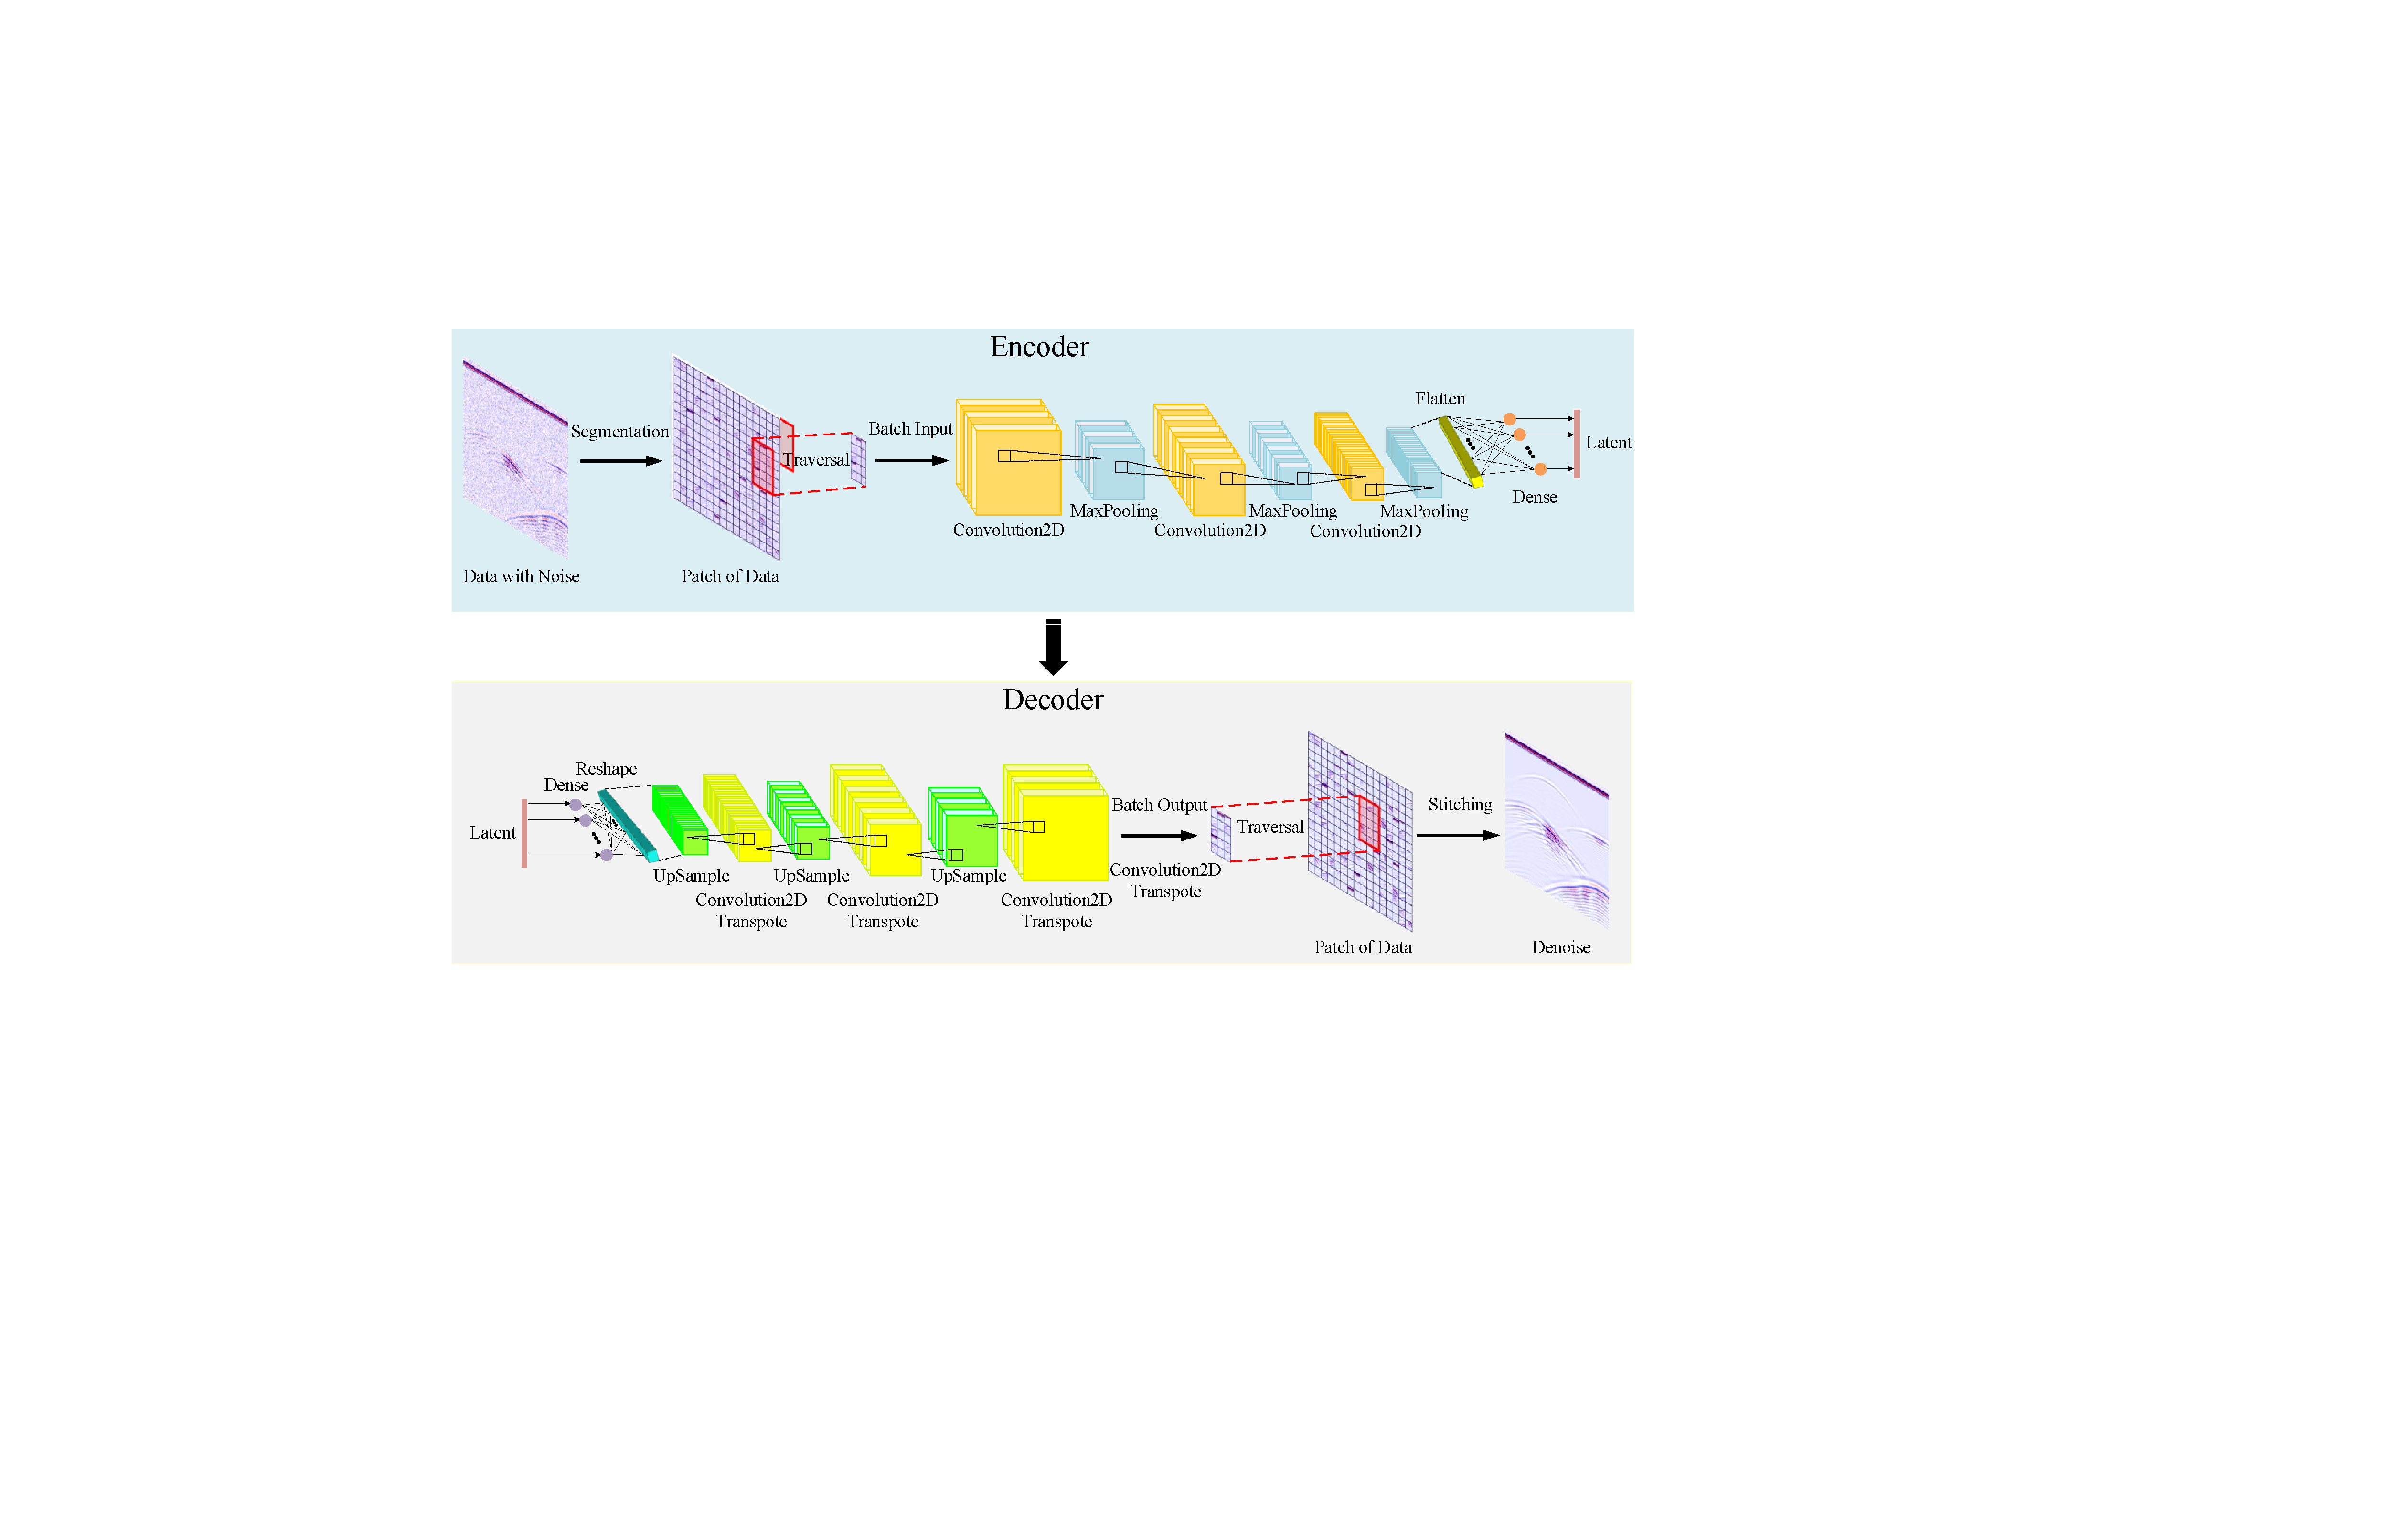
\includegraphics[width=5.5in]{./FigureFolder/CDAEs/StructureOfCDAEs.pdf}
\caption{传统CDAEs网络结构}
\label{Fig_CDAEs}
\end{figure}
\par
对于地震剖面数据而言,数据本身所含有的有效特征信息很少,大部分数据为冗余信息,并且更加容易触发深度学习中梯度爆炸和梯度消失的问题,因此,传统的网络架构对于地震数据并不适合,需要对网络结构进行优化,从而根据地震数据的特点达到自适应的目的。
\par
2) 去除直达波的Wave-U-Net神经网络构建
\par
地震直达波的存在会对偏移效果产生极大的影响,体现在表层过度照明,导致深层信息完全被覆盖,从而无法获得深部信息,因此,找到一种能够良好去除直达波,并且对其他波形没有影响的方法是至关重要的,常用的去除直达波的方法有SVD变换、Radon变换、FFT变换等方法,然而这些方法都是基于域变换的,不仅需要人工处理异常波形,最大的缺陷是无法将波形彻底分离,存在波形特征重叠的现象。
\par
因此,找到一种能够完美分离波形的新算法是十分必要的,受音频数据分离的启发,构建了一种名为Wave-U-Net的神经网络结构用于去除地震直达波,它是U-Net对一维时域的一种改编,它会重复对特征图进行重新采样以计算和组合不同时标的特征。为了获得更加良好的去除效果,可以对体系结构做进一步改进,包括强制执行源可加性的输出层,上采样技术和上下文感知预测框架以减少输出伪像。
\par
Wave-U-Net架构图如图\ref{Fig_U-Net}所示。它使用降采样(DownSample, DS)块在较粗的时间尺度上计算出越来越多的高级特征。这些特征与使用上采样(UpSample, US)块的较早计算的局部高分辨率特征相结合,产生用于进行预测的多尺度特征。该网络总共有$L$个级别,每个连续级别的时间分辨率是前一个级别的一半。
\par
\begin{figure}[htbp]
\centering
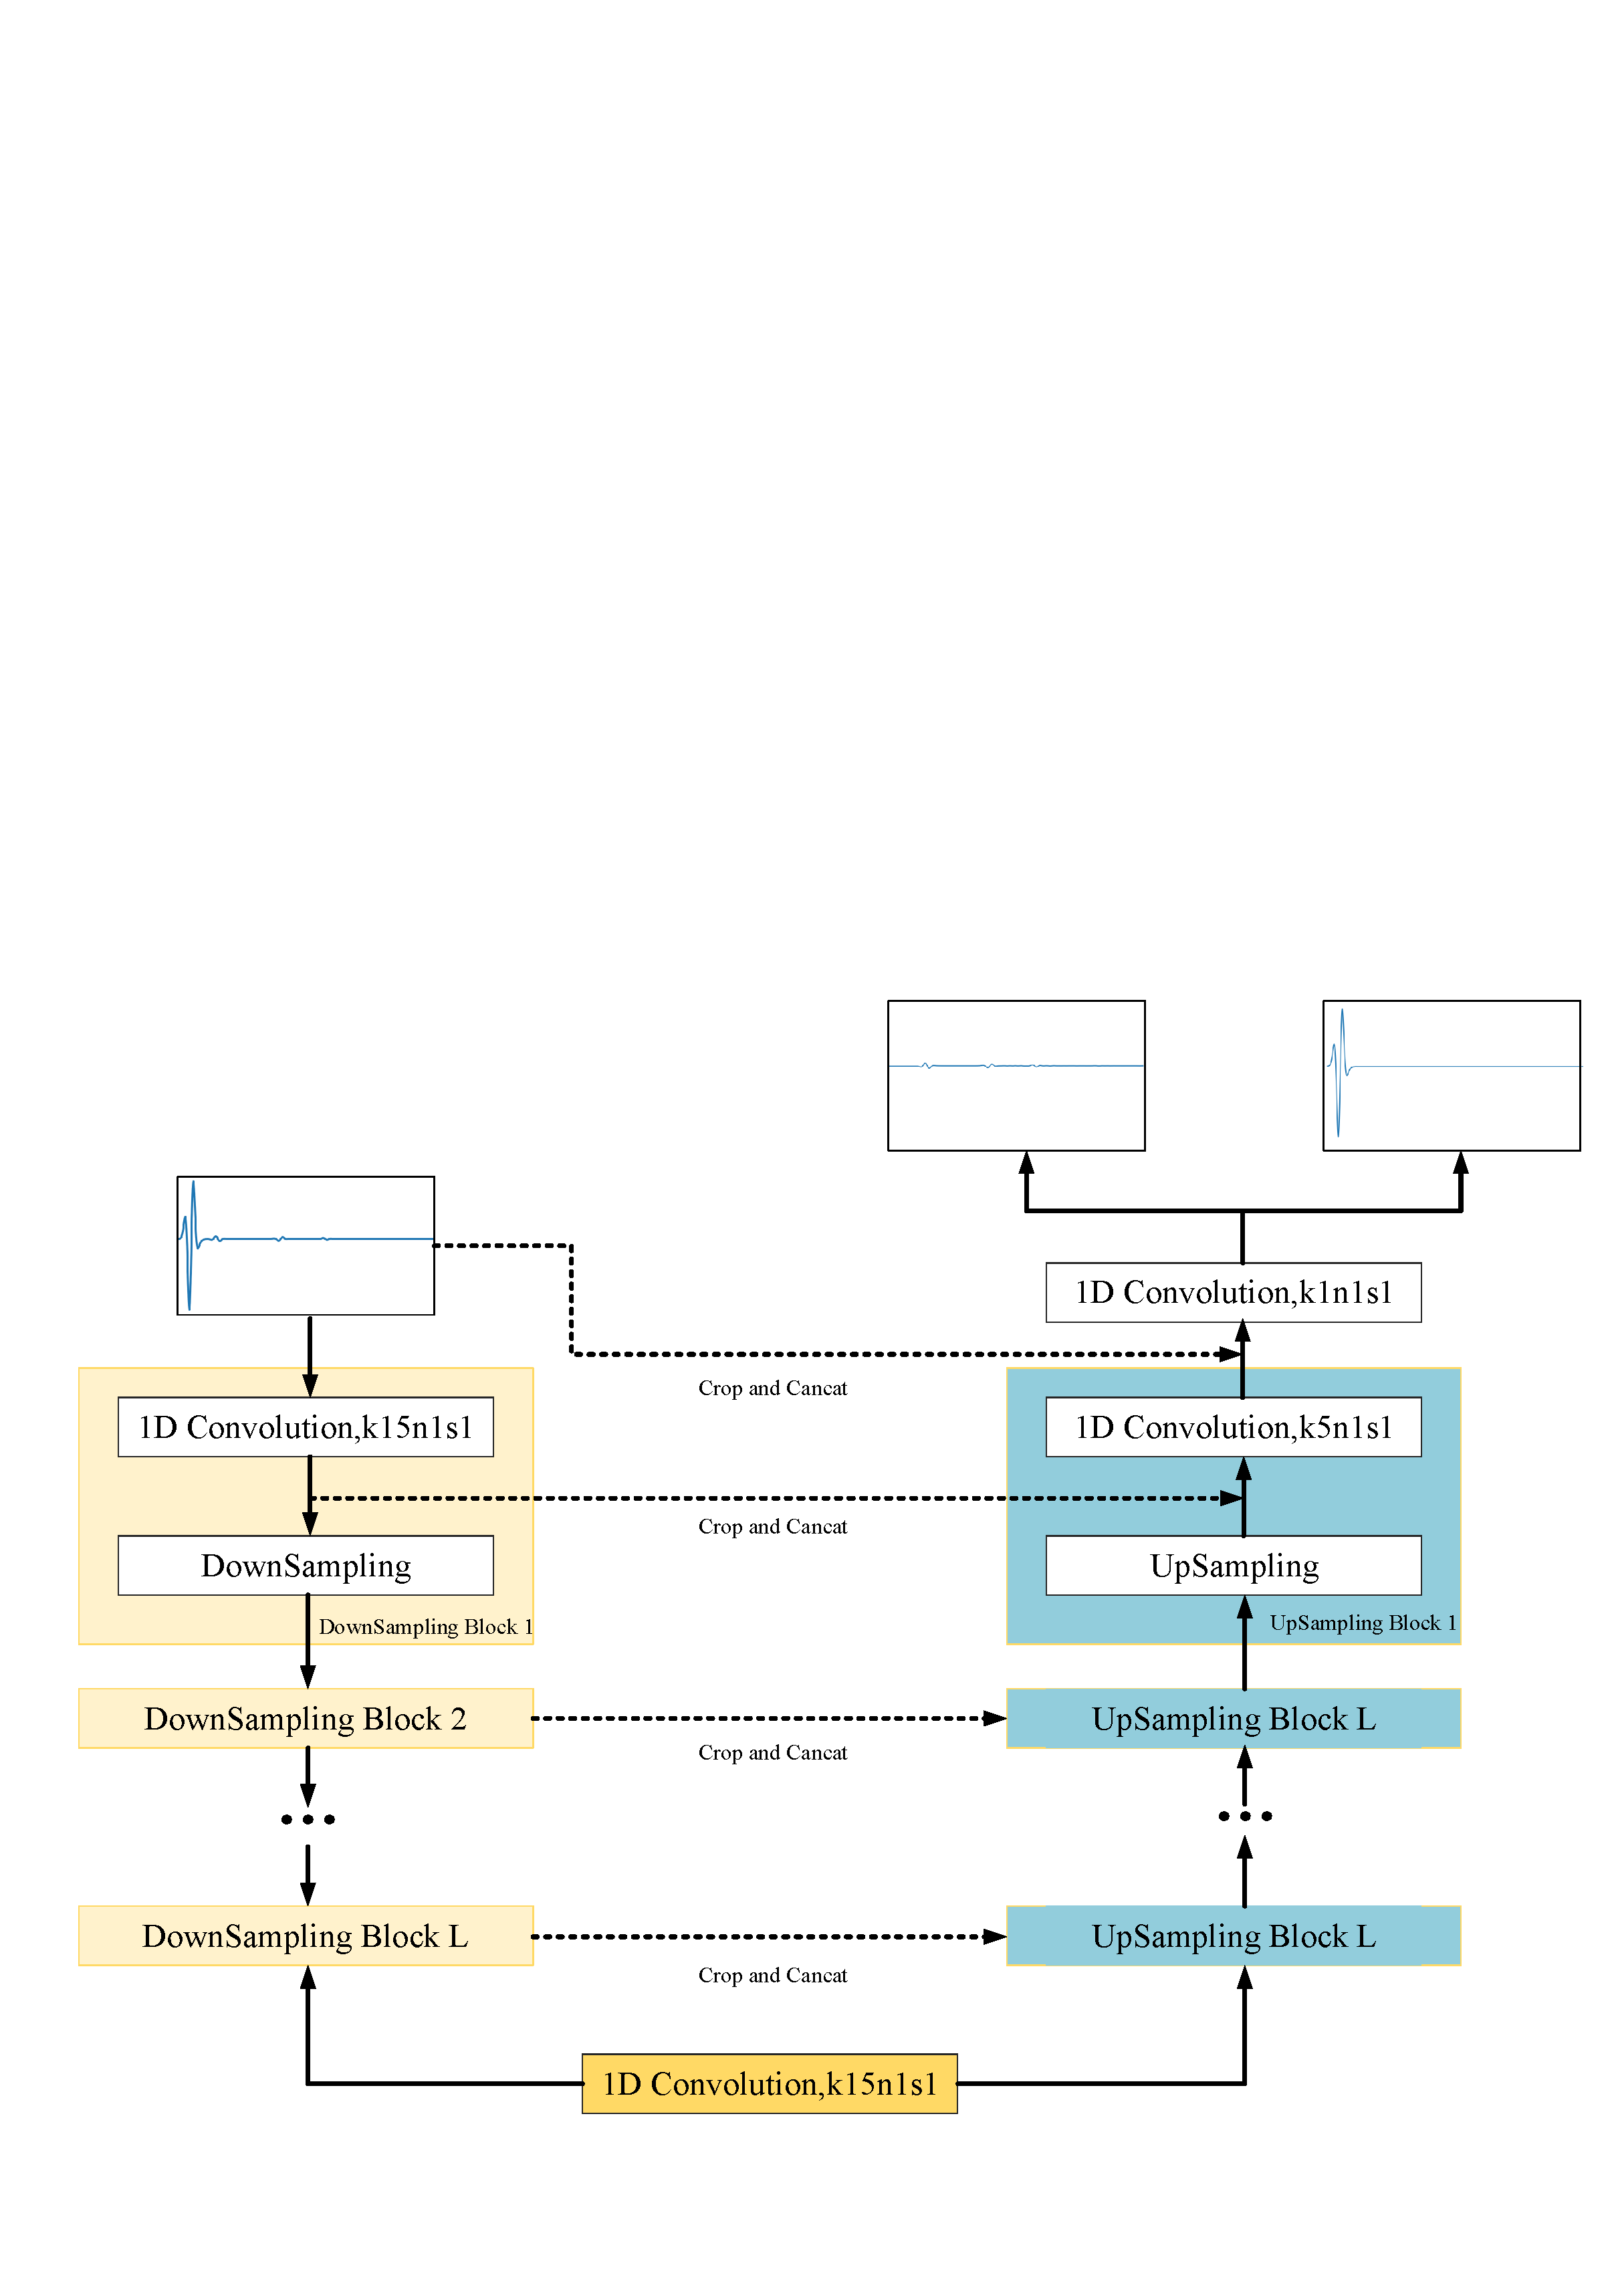
\includegraphics[width=5.5in]{./FigureFolder/U-Net/UNet.pdf}
\caption{Wave-U-Net网络结构}
\label{Fig_U-Net}
\end{figure}
\par
通过建立学习样本集,不断更新迭代计算Wave-U-Net的权重值及偏置值,在不损失有效波形信息的同时,完美地将直达波进行分离。
\par
3) 基于压缩感知算法的低内存高效地震逆时偏移算法
\par
在进行了波场正向外推和逆时外推,我们记录了每一时刻的波场信息,接下来就是对前两步得到的正逆向外推数据进行成像。成像需要用到成像条件,成像条件的运用是逆时偏移过程中的一个重要流程,逆时偏移最终目的是要获得成像剖面。Clarebout认为,反射面在地层中位于上行波场与下行波场交汇的地方,表现在时间上就是在两个波场时间相同的时刻处。根据Clarebout这一原理,主要应用的经典的成像条件基本有,互相关成像条件,激发时刻成像条件以及上下振幅比成像条件。如图\ref{Fig_Migration}所示,蓝色的成像点的位置就是在由震源激发的波场,和检波点波场,延拓时间相一致的地方,将整个计算区域,运用时间一致性原理,就能得到全部的反射点,这些反射点就构成了反射界面。正是因为如此,偏移成像才能够成为地震数据处理的三大重要技术之一,逆时偏移成为地震勘探获取地下构造信息的一种有效手段。
\par
\begin{figure}[htbp]
\centering
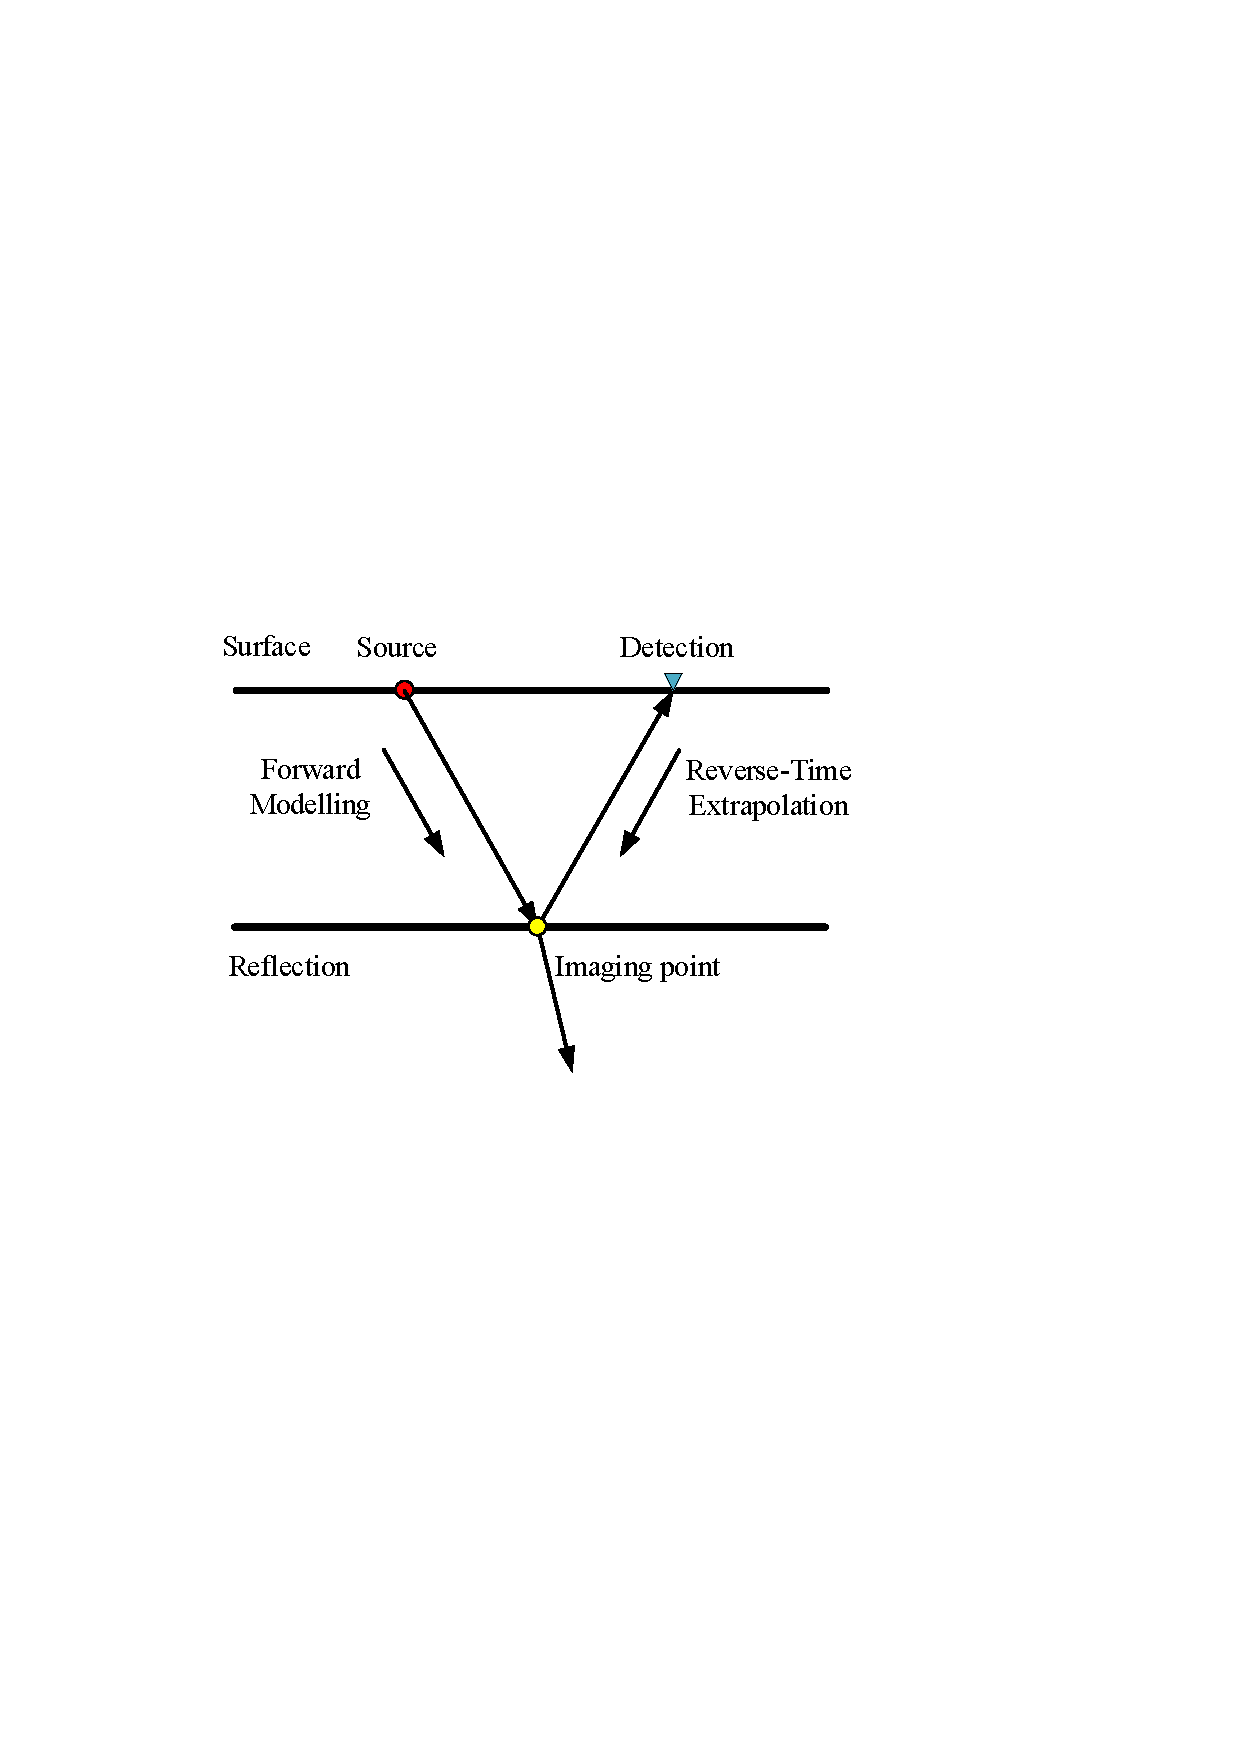
\includegraphics[width=3in]{./FigureFolder/RTM/Migration.pdf}
\caption{偏移成像示意图}
\label{Fig_Migration}
\end{figure}
\par
a) 激发时间成像条件
\par
激发时间条件是Sun于1986年首次提出,Huygens原理告诉我们,当波在地下介质中传播时,波传播所经过的点,都可以视作一个新的波源,这些新的波源和震源一样会向各个方向发出能量更微弱的二次波。根据这一原理,地震记录既可以视作是由震源激发的地震波对地下介质的响应,也可以视作是地下介质中各点在不同时刻激发不同强度的二次波传播到检波器所在位置进行的叠加。所以检波器记录到的记录可以理解为是地下所有绕射点的绕射波的叠加。结合时间一致性原理激发时刻成像条件认为直达波的初至时间就是成像时间,如果在某些位置处绕射波产生的时间恰好等于直达波到达的时间,那么这些点的位置就在反射层上。所以激发时刻成像条件的目的就是找到直达波波至时刻,激发时刻成像条件根据寻找初至方法的不同可以分为两种,一种是利用射线法获取初至走时成像条件,另一种是利用有限差分法获取初至走时成像条件。
\par
基于射线法的射线追踪初至成像条件步骤:
\par
(1)通过射线追踪得到走时曲线,得到初至时间;
\par
(2)将检波点波场逆时反推,从记录的最大时刻开始递减外推;
\par
(3)在反推的过程中每一时刻运用成像条件,并对其求和;
\par
基于有限差分法的最大振幅成像条件步骤:
\par
(1)通过数值波场模拟,通常是有限差分法求取最大振幅时刻,将该时刻作为初至时刻;
\par
(2)将检波点波场逆向外推,从记录的最大时刻开始递减外推;
\par
(3)对每一时刻运用成像条件,累计求和,获得最终成像结果;
\par
激发时刻成像条件的存储量小,不需要保存每一时刻的波场信息,计算效率比较高,当模型不是特别复杂的时候可以选取这种成像方法;但是它的缺陷也非常明显,当地层结构变得比较复杂,使用激发时刻成像条件会存在多波至问题,这时就无法准确的获取初至,从而会产生一些虚假的成像点。由于该方法没有保存完整的波场信息,并未充分利用波场信息,在这种多波至情况下将无法排除掉虚假的成像点,将导致偏移结果变差。
\par
b) 上下行波振幅比成像条件
\par
该方法认为,反射界面就是所在的地方就是下行波场和上行波场在时间与空间上重合的地方,也就是说反射点必定是那些上下行波场时间完全相同的点。其计算原理如式(\ref{eq_AmplitudeRatio})所示:
\begin{equation}\label{eq_AmplitudeRatio}
image(x,z)=\frac{u(x,z,t)}{d(x,z,t)}
\end{equation}
上式中分子,分母分别为上,下行波场。这个方法通常不单独使用而是依赖于其他成像条件,经常被用来估算界面反射系数。
\par
b) 互相关成像条件
\par
Claerbout于1971年首次提出互相关成像条件,Whitemore在1986年将互相关成像条件应用到了逆时偏移中。反射界面位于地层内正向外推波场和逆时外推波场时间相一致处。时间一致性原理在数学计算上的直接表现方式就是零延迟互相关函数。其具体表达式为式(\ref{eq_Correlation})所示:
\begin{equation}\label{eq_Correlation}
image(x,z)=\int_0^T u(x,z,t) d(x,z,t) dt
\end{equation}
式中 $u(x,z,t)d(x,z,t)$表示在计算过程中某一时刻对模型计算区域内整个波场做一次成像计算,对时间变量t 求和的含义是对波场计算过程中的所有时刻进行叠加求和,整个公式表明互相关成像条件是对全时刻,全空间累计求和,所以说互相关成像条件在成像过程中利用了全部时间和空间完整的波场信息进行成像运算。
\par
互相关成像条件步骤:
\par
首先离散应力-速度波动方程,按照精度要求对波动方程进行高阶时空差分,正演计算得到正向波场,保存每一时刻的波场信息;
\par
将正演得到的地震记录信息作为波动方程的边界条件,逆着时间方向,从最大时刻处逐步计算直至0时刻,获得每一时刻的逆时波场信息,并保存;
\par
提取出同一时刻的正向波场,和逆时波场,对同时刻的两个波场做互相关运算,再遍历每一时刻,对所有时刻两个同时刻波场互相关的结果累计求和,得到单炮偏移结果。
\par
互相关成像条件的优点显而易见,它保存了每个时刻的波场信息,计算精度相比于激发时刻条件更为精确。不过互相关成像条件也存在一些问题,在进行互相关成像时,通常情况下弹性界面的反射参数不能相差过大。如果弹性界面两侧波阻抗差异较大时,由于强烈的层间反射会导致偏移噪声变强,保幅性变差,偏移质量变差。
\
从以上描述可以看出,采用互相关成像条件时需要保存正演和逆时两个过程的波场信息,这个过程导致占用极大的物理内存,从而降低偏移的效率。
\par
受到图像信号处理算法的启发,可以考虑将图像压缩算法引入逆时偏移计算中,图像信号处理是对原始信号进行采样、变换、提取的过程。在此过程中,信号会由某些特定变换域表示\upcite{WangB2018}。较为典型的变换域包含时域、空间域和频域等。通常在时域内信号是非稀疏的,但在其他的变换域中就有很大几率是稀疏的。在此理论的支撑下,选取一组正交基的变换便可求解稀疏系数\upcite{ZhangQ2018}。在某变换域上,信号的稀疏表示可以让大部分的系数为零,其中仅有一小部分的系数不是零。在此情况下,原始信号就能够投影到低维空间中转换成稀疏信号。在求解一个优化问题后,可从少数的投影中重构原始信号。换言之,其主要思想就是通过一种更为有效的方式描述信息,使用更少的基向量来重构原始信息特征,根据这种思想,我们就可以将波场数据进行压缩处理,极大地降低物理内存的消耗,从而提高逆时偏移的计算效率。
\par
稀疏表示的基本原则时将自然信号由一个基函数字典现行叠加表示\upcite{Loxley2017},已有信号$Y \in R^n$,基函数字典$D=\{ d_1,d_2,\cdots,d_m \} \in R^n$,在稀疏表示模型中,$Y$可以表示为:
\begin{equation}\label{eq_SignalY}
\min \parallel X \parallel_0 \quad s.t. Y=DX
\end{equation}
式(\ref{eq_SignalY})中,$X$表示的含义时稀疏编码,$\parallel X \parallel_0$为向量的$l_0$范数,表示的是$X$中非零元素的个数。
\par
若字典$D$的维度大小是$n > m$,线性方程$Y=DX$可求解出唯一解,若字典维度大小是$n < m$,字典的列数多与行数,满足过完备字典的要求,在过完备字典的情况下,线性方程具有不唯一的解$X$。为完成优化,可添加约束条件,如式(\ref{eq_Condition})所示:
\begin{equation}\label{eq_Condition}
\min \parallel Y-DX \parallel_2^2 \quad s.t. \parallel X \parallel \leq k
\end{equation}
式(\ref{eq_Condition})中的稀疏模型是约束在线性组合不超过$k$个原子的基础上完成的,这会让误差尽可能小,由上可知,稀疏表示问题的核心环节是稀疏表示系数的求解是否能够正确和过完备字典的构建是否达到最优\upcite{SunJ2017}。
\par
Elad等\upcite{Aharon2006}(2006)提出K奇异值分解(K-Singular Value Decomposition, K-SVD)算法,是目前为止求解过完备字典效果较好的方法之一,K-SVD算法是对字典原子逐列更新,综合考虑了字典原子对每一个训练样本的影响,增强了字典原子的描述能力。
\par
字典学习的最终目的是训练出过完备字典矩阵$D \in R^{n \times K}$,其中有$K$个字典原子。K-SVD字典学习算法是K-means算法的一种推广,K-SVD算法的目标函数\upcite{HongT2016}如(\ref{eq_KSVD0})所示:
\begin{equation}\label{eq_KSVD0}
\min_{D,X} \{ \parallel Y-DX \parallel_F^2 \} \quad s.t. \forall i,\parallel x_i \parallel_0=1
\end{equation}
式(\ref{eq_KSVD0})中,$F$代表的含义是Frobenius范数。
\par
为了在字典$D$中实现原子的线性组合,约束的稀疏项被放宽,让每列$x_i$中的非零个数多于1,这便会有约束条件,必须要求$x_i$中的非零个数小于$T_0$,$T_0$表示的含义是稀疏系数向量中的非零元素的数量。那么,目标函数可写为:
\begin{equation}\label{eq_KSVD1}
\min_{D,X} \{ \parallel Y-DX \parallel_F^2 \} \quad s.t. \forall i,\parallel x_i \parallel_0=T_0
\end{equation}
\par
在稀疏编码阶段,固定初始化字典$D$,选用正交匹配追踪(Orthogonal Matching Pursuit, OMP)算法计算最佳稀疏编码矩阵$X$。
\par
在字典更新阶段,以求解得到的最佳稀疏编码矩阵$X$为基础,更新自适应字典。K-SVD算法采用的更新方式是逐列更新,因此,在更新某一列时,惩罚项可转换为:
\begin{equation}\label{eq_KSVD2}
\parallel Y-DX \parallel_F^2=\parallel (Y-\sum_{j=1}^K d_j X_T^j) \parallel=\parallel (Y-\sum_{j \neq k}^K d_j X_T^j)-d_k x_T^k \parallel_F^2=\parallel E_k-d_k x_T^k \parallel_F^2
\end{equation}
其中,$x_T^k$时稀疏矩阵$X$中的第$k$行向量,矩阵$E_k$表示的含义时除第$k$个字典外所有的$N$个样本的误差项。
\par
在此情况下,直接采用SVD算法更新$d_k$和$x_T^k$,能够求解得到和$E_k$距离最小并且秩为1的矩阵,但是其中的$x_T^k$不一定稀疏,所以更新的$d_k$不满足稀疏条件。那么,就需要$x_T^k$中仅保留非零项,然后再用SVD更新$d_k$和$x_T^k$。从而,构建集合$\omega_k=\{ i|1 \leq i \leq N,x_T^k(i) \neq 0 \}$,$\omega_k$表示的是$x_T^k(i) \neq 0$的点的索引值,设定矩阵$\Omega_k$的大小为$N \times |\omega_k|$,若在点($\omega_k(i),i$)的位置是1,则在其他位置点是0。定义$x_R^k=x_T^k \Omega_k$,$Y_R^k=Y \Omega_k$,$E_R^k=E_k \Omega_k$,$Y_R^k$为原子$d_k$样本的集合,$E_k$是$E_R^k$除去不受原子$d_j$影响到的样本外其他原子带来的误差,可以将式(\ref{eq_KSVD2})转换为:
\begin{equation}\label{eq_KSVD3}
\parallel E_k \Omega_k-d_j x_T^k \Omega_k \parallel_F^2=\parallel E_R^k-d_k x_R^k \parallel_F^2
\end{equation}
\par
接下来对$E_R^k$进行奇异值分解,则$E_R^k=U \Delta V^T$,设定$\tilde{d}_k$表示为$U$的第一列,那么$\tilde{d}_k$的具体含义就是$d_k$更新的结果。并在此时,选用$V$的第一列和$\Delta (1,1)$两者之间的乘积更新$E_R^k$。直到达到条件之后才可以停止重复迭代过程。
\par
4) 低频数据预测器的构建
\par
采用局部最优化算法求解时,会很容易陷入局部极小值,因此,提出了多尺度串行全波形反演策略,由于声波数据中的低频分量主要包含地下较大的构造体信息,而高频分量包含较小构造体的细节信息。因此,首先反演声波数据中的低频分量从而得到一个较好的反演模型,然后将这个反演模型当作声波数据中高频分量的反演初始模型,最终得到高频分量的反演结果,这样,将高、低频分量结合起来进行多尺度串行全波形反演,能够有效提高反演结果的精确性。通常采用Wiener低通滤波器\upcite{Hansen1989,Portilla2001,King1984},它将反演问题分解为不同的频率,对观测数据与震源子波滤波得到低频带信息,采用2-4个低频带到高频带的逐频带反演,根据不同频率尺度上的反演目标函数的特征去求解反演问题,从而逐步搜索到全局极值点,避免陷入局部极值。
\par
这样的处理方法需要将数据进行两次变换,计算效率较差,因此,采用基于神经网络的数据预测算法,通过迭代计算出合适的权重值和偏置值,从而将输入的高频数据直接变换到需要的频率数据,进而提高计算效率。
\par
论文拟采用卷积自动编码器法对数据进行频率转换,实现高频到低频数据的预测。采用卷积层将自动编码器设计为一个卷积自动编码器。对于如图\ref{Fig_Encoder}所示的编码器部分,首先将地震剖面数据提取为单道波形,经过卷积层、池化层和全连接层之后转换为一个低维潜向量;对于如图\ref{Fig_Decoder}所示的解码器部分,可理解为编码器的反向操作,解码器接收一个低维潜向量,最终输出为变换后的波形,最终组合成为变换后的地震剖面;具体的卷积操作如图\ref{Fig_Conv}所示。
\par
\begin{figure}[htbp]
\centering
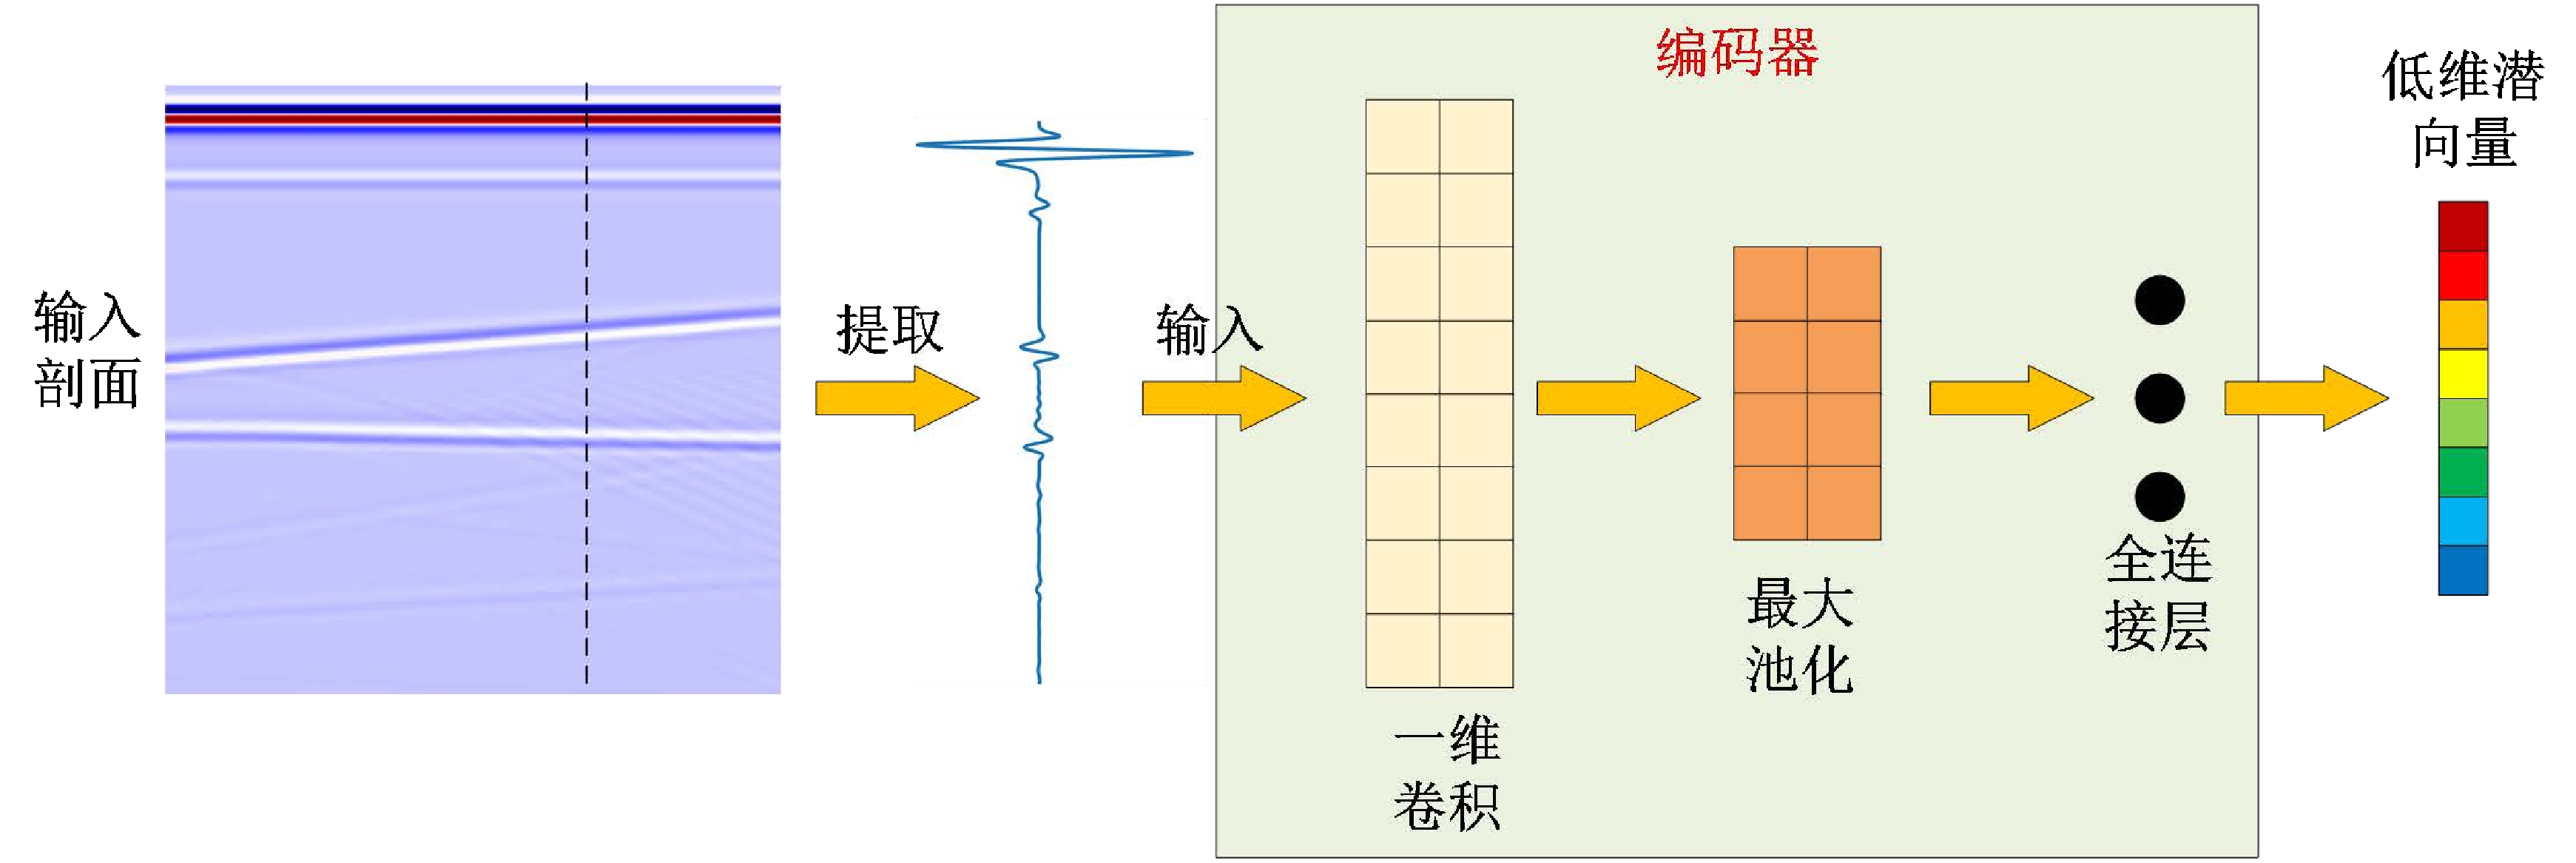
\includegraphics[width=4in]{./FigureFolder/Predict/Encoder.pdf}
\caption{编码器示意图}
\label{Fig_Encoder}
\end{figure}

\begin{figure}[htbp]
\centering
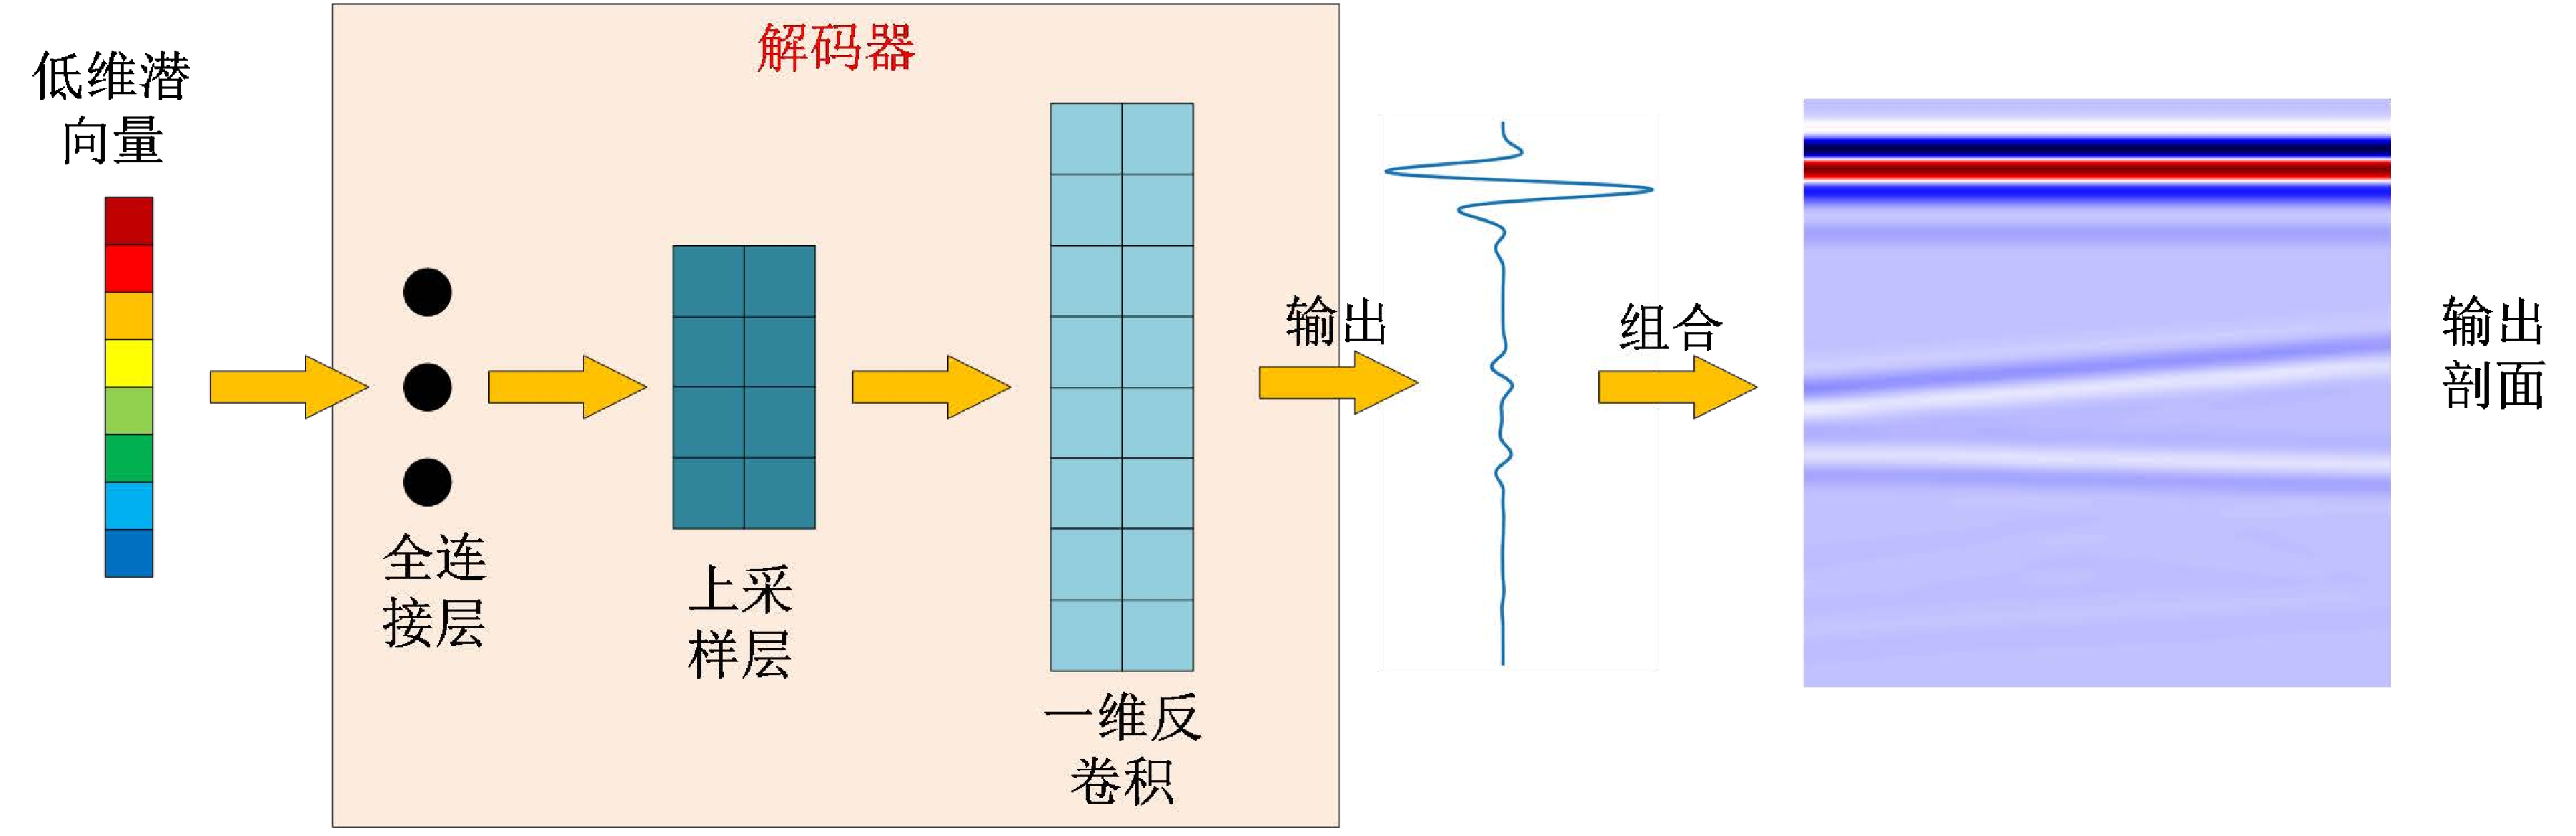
\includegraphics[width=4in]{./FigureFolder/Predict/Decoder.pdf}
\caption{解码器示意图}
\label{Fig_Decoder}
\end{figure}

\begin{figure}[htbp]
\centering
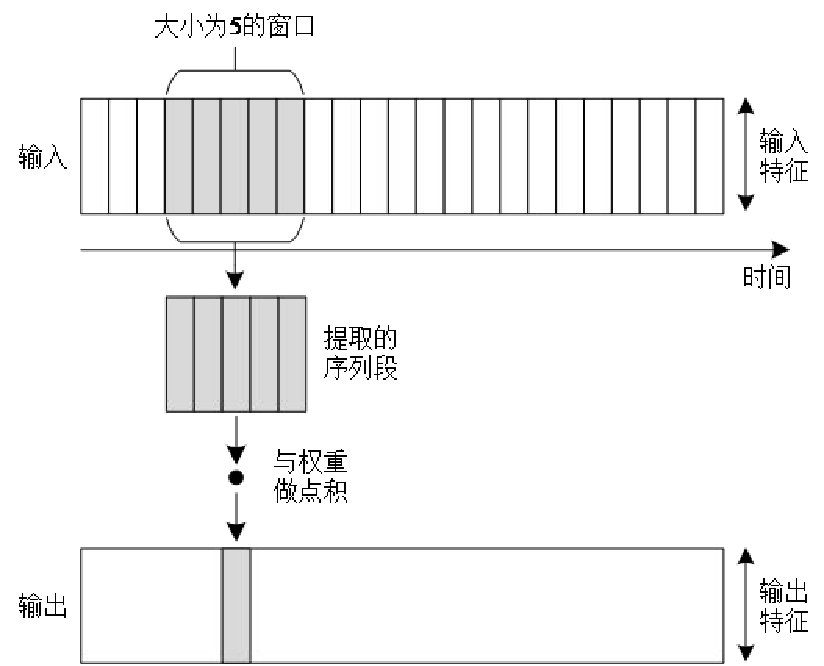
\includegraphics[width=4in]{./FigureFolder/Predict/Conv.pdf}
\caption{卷积操作示意图}
\label{Fig_Conv}
\end{figure}
\par
这样就可以实现一个端到端的频率变换映射,从而提高了频率转换的效率。
\par
5) 超分辨率地震处理的空间多尺度全波形反演算法
\par
使用频率多尺度全波形反演方法,由于反演过程需要进行由低频到高频的逐频数据反演,在使用低频数据时,由于低频数据的分辨率较低,因此只需要使用粗网格即可达到相应频率的分辨率要求,若采用细网格非但不能有效提高反演精度,而且还会造成物理内存的浪费,从而降低反演效率;而随着地震数据频率的提高,对网格的要求也随之提高,此时需要使用细网格进行剖分以达到当前频率的分辨率要求,针对这个需求,这就需要将粗网格数据无损地映射到细网格上,映射通常使用双三次插值完成,但是由于双三次插值会造成原始信息的缺失,因此需要使用精度更高的算法来实现网格间的映射,采用超分辨率算法能够很好地满足这个需求,并且能够有效地提升全波形反演的计算效率。
\par
从对应的低分辨率图像重建高分辨率的逼真图像一直是计算机视觉界的一项长期挑战。当仅有一个低分辨率图像作为重新创建其高分辨率图像的输入时,此任务将变得更加困难。从单个低分辨率(Low Resolution, LR)副本中提取高分辨率(High Resolution, HR)图像的估计称为超分辨率(Super Resolution, SR)。在地震反演的角度上来说,LR对应的是粗网格数据,HR则是细网格数据,而SR是预测的细网格数据。当应用机器学习解决方案时,LR图像通常是降采样后的HR图像,并带有一些模糊和噪声。
\par
首先,非常早期的解决方案是图像处理中的插值方法。在此,使用某些插值方法(例如最近邻,双线性或双三次插值方法)将低分辨率图像的大小调整2倍或4倍,这种方法处理的结果通常是模糊的,并且存在数据的缺失。
\par
随着全卷积神经网络(Full Convolutional Neural Network, FCNN)在解决语义分割方面的成功,它在计算机视觉的其他领域的普及迅速普及。FCNN是一个CNN,在其后面没有任何密集的连接(完全连接的层)。每个CNN都有两个主要功能块,即
\par
i) 特征提取器;
ii) 分类器。
\par
CNN后面的密集连接是分类器,其任务是将提取的特征映射到类概率。FCNN是从输入图像生成/预测输出图的基本设计实践。输出图可以是语义分割图,样式转换图像甚至是超分辨率图像。换句话说,FCNN是图像到图像的映射引擎。Super-Resolution Convolutional Neural Network(SRCNN)是FCNN在超分辨率中的初步应用之一。
\par
在SRCNN中,首先使用双三次插值对图像进行上采样,然后馈入简单的FCNN。重要的是要注意,不涉及池化操作。因此,导致输出具有与上采样的输入图像相同的空间尺寸的输出。最后,我们计算目标HR图像与输出之间的MSE损失。
\par
使用SRCNN在单个图像上获得了超分辨率的成功\upcite{DongC2014},启发了其他人带来了进一步的体系结构改进。众所周知,Residual Network(ResNet)比常规的CNN更好。SRResNets用残差块代替了简单的卷积块。结果准确性显着提高。但是,正如人们可能已经观察到的那样,采用跨步卷积梯度实现的上采样操作会增加零值以放大图像,以后必须用有意义的值填充该值。甚至更糟的是,这些零值没有可以反向传播的梯度信息。
\par
为了避免这个现象,使用相移的图像重塑,也称为``像素混洗''(Pixel Shuffler)的方法来解决上采样问题\upcite{ShiW2016}。
\par
随着对生成对抗网络的不断研究,GAN提供了一个强大的框架,可以生成具有高感知质量的看起来合理的自然图像。GAN程序鼓励重构物向搜索空间区域移动,从而很有可能包含照片级逼真的图像,从而更接近自然图像流形。SRGAN是一个基于GAN的网络\upcite{Ledig2017},其中生成器(G)学习从尽可能接近HR的LR图像生成SR图像。鉴别器(D)学会将生成的SR图像与真实图像区分开。G利用ResNet和亚像素卷积进行上采样。它还将感性损失与生成性或对抗性损失相结合,以计算其损失,SRGAN的一般架构如图\ref{Fig_GAN}所示。
\par
\begin{figure}[htbp]
\centering
\includegraphics[width=5in]{./FigureFolder/Predict/GAN.pdf}
\caption{超分辨率生成对抗网络结构图}
\label{Fig_GAN}
\end{figure}
\par
6) 基于模型预测器的全波形反演约束的构建
\par
在反演的迭代过程中增加模型约束能够是反演更加准确并且增加反演的稳定性,常规的约束方法有Tikhonov正则化约束、TV正则化约束、MTV正则化约束等,这些正则化模型约束方法往往针对特定的模型才具有行之有效的作用,对于结构复杂的地下模型则会显示出单独方法的不足之处,Tikhonov正则化约束会使得界面过度光滑,而TV正则化、MTV正则化约束则会导致界面过度锐利,对于复杂模型,仅仅使用一种约束策略显然是不够的,然而建立一个混合约束不论从效率还是从精度来讲都具有较差的反应,因此建立一个符合地下构造的模型预测器是十分必要的。
\par
模型预测器选取特殊的地下结构作为学习样本,尽可能符合地下实际模型,在反演迭代的过程中对反演迭代数据使用模型预测器不断进行优化,从而对其施加模型预测约束,使得反演数据尽量符合地下实际构造,提高反演的准确性。
\par
地质构造学习样本集如图\ref{Fig_Model}所示,从图中能够明显看出,学习样本集中具有很多特殊的地质构造信息,例如断层信息、向/背斜信息、起伏地形信息、空洞信息以及常见的均一介质信息等。
\begin{figure}[htbp]
\centering
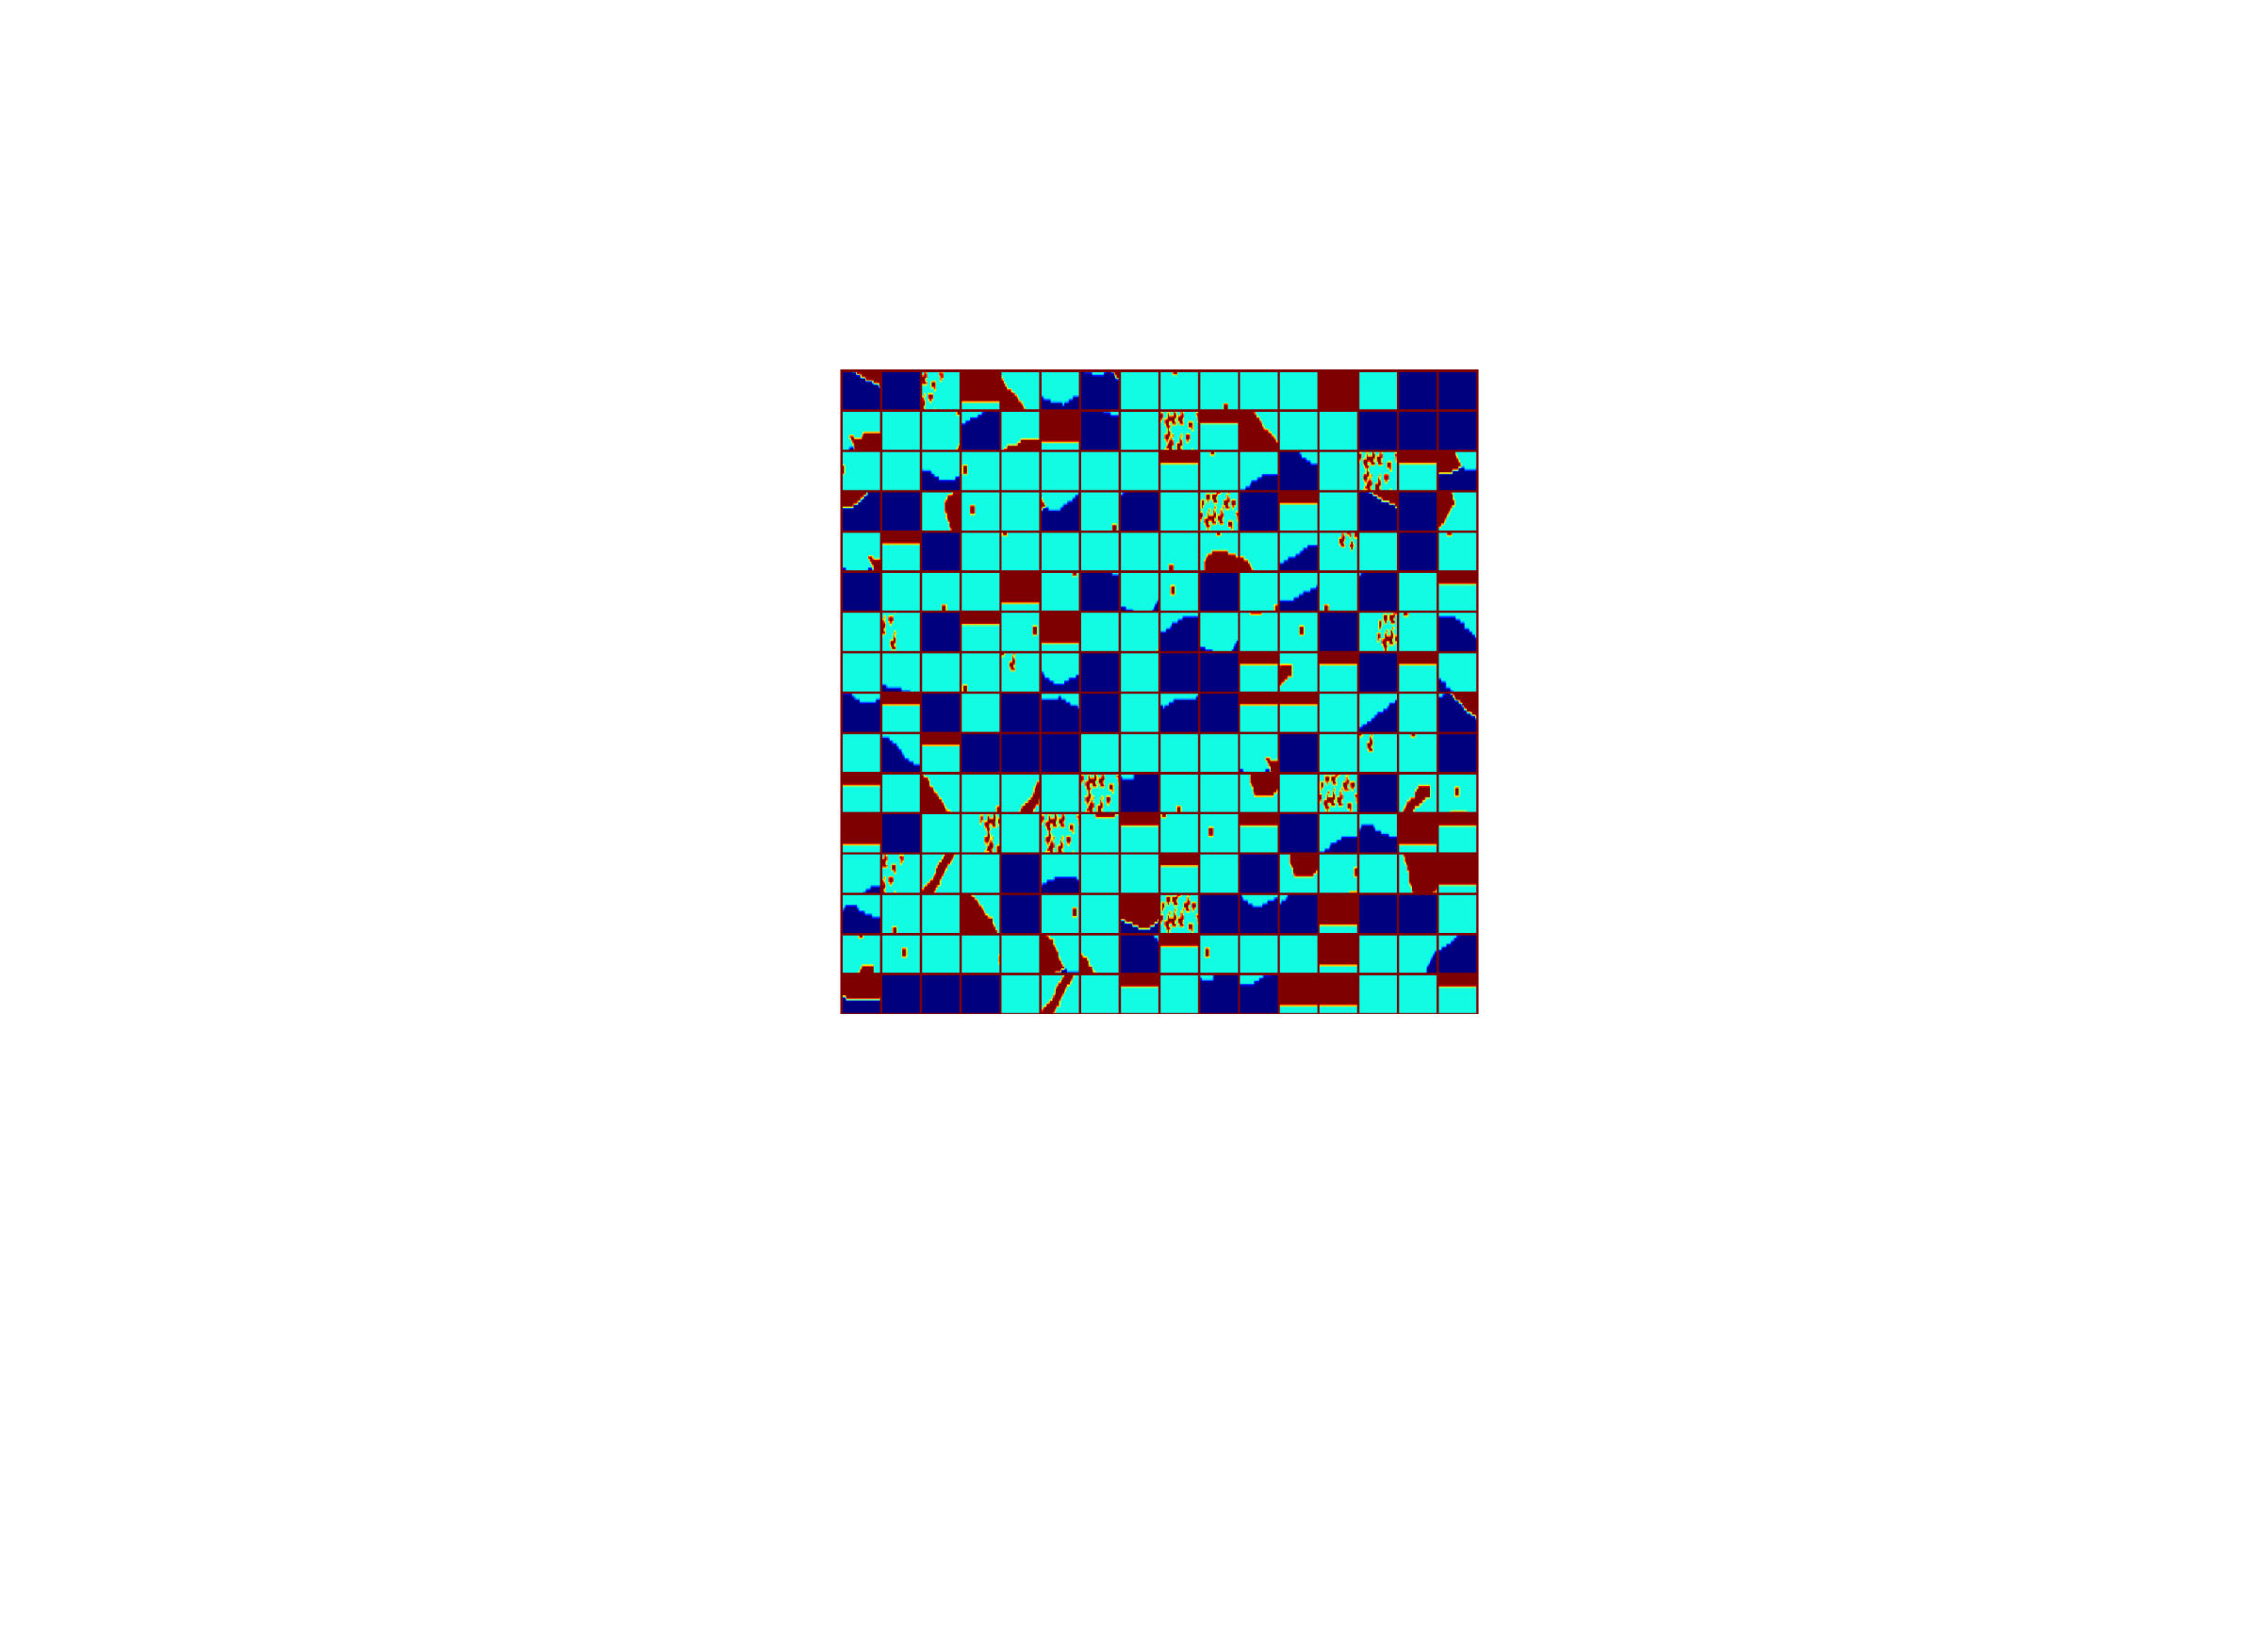
\includegraphics[width=2in]{./FigureFolder/Predict/Model.pdf}
\caption{地质结构学习样本集}
\label{Fig_Model}
\end{figure}
\par
\subsection*{\kai\fontsize{11pt}{10pt} \selectfont【创新点】}
1) 采用CDAEs及Wave-U-Net对地震数据进行端到端的处理,达到了高保真无损处理地震数据的目的。
\par
使用结构优化的深度卷积自动编码器达到了地震数据高保真无损去噪的目的,将深度学习算法与地球物理数据处理相结合,并对CDAEs进行了结构调整,使其更加贴合地球物理数据;构建适合地震数据的Wave-U-Net神经网络模型对地震剖面数据进行去除直达波处理,同时可以将其扩展到例如分离上下行波等其他领域,为地震高精度偏移奠定基础;建立适合地震数据的预测神经网络模型对地震剖面进行高频到低频的快速转换,实现了端到端的频率转换方法。
\par
2) 采用K-SVD压缩感知算法对波场数据进行稀疏表示,达到了低内存消耗的高效地震逆时偏移的目的。
\par
将压缩感知算法与地球物理方法相结合,极大地降低了地球物理算法对于计算机的要求,使地震处理能够在普通计算机上得到良好的应用,并且还可以将这种思想扩展到例如全波形反演等其他领域,极大地提高了地震数据处理的效率。
\par
3) 提出了全新的多频率多空间尺度的模型约束全波形反演算法。
\par
使用超分辨率的思想实现了数据由粗网格到细网格的端到端的映射,从而实现了多空间尺度的全波形反演算法,大大提升了全波形反演算法的效率,降低了全波形反演对于计算机内存的消耗;同时提出了模型约束的全波形反演约束策略,不再利用单一的正则化方法对反演结果进行约束,而是采用接近地下模型的样本集对反演结果进行优化处理,结合了多种正则化约束策略的优点,提高了全波形反演的精度;综上所述,新的算法不仅能够提升全波形反演效率还能提升全波形反演的精度。
\par
\newpage
\section*{\hei\fontsize{11pt}{10pt} \selectfont \\ 四、拟采用的研究方法和技术路线}
\subsection*{\kai\fontsize{11pt}{10pt} \selectfont【基于CDAEs的地震剖面去噪】}
1) 学习数据集的建立
\par
为了对卷积去噪自动编码器进行训练,随机生成200组地震剖面,其中包括100组随机不规则地下异常体模型和100组随机地形起伏异常模型,两类模型的异常体数量、异常体形状、异常体大小、异常体位置及异常体参数均为随机生成,这样做的目的在于能够避免相同的波形特征被重复学习,同时也能够获得更多的波形特征以便神经网络能够学习更多的特征信息。通过对异常体的地震剖面施加不同噪声等级的高斯噪声,并且使用窗口滑动的方法剖分成多个窗口滑动块来获得关于波形细节的波形特征样本数。
\par
使用块数据而不是整个剖面数据的目的有两个,一是地震剖面是冗余的,大部分数据是无效的,将地震剖面分成数据块能够更好地避免数据冗余,从而使波形特征能够得到更好地学习;二是获得了更多的学习样本,将数据分成数据块能够使用较少的剖面数据产生更多的学习样本。
\par
2) 网络结构优化
\par
为了获得对地震数据更好的适应性,因此需要对网络结构进行优化,从局部感受野、正则化方法的添加和网络结构等方面进行优化,通过调节网络结构及网络参数获得最优的去噪效果。

\subsection*{\kai\fontsize{11pt}{10pt} \selectfont【基于Wave-U-Net的地震剖面直达波去除】}
1) 学习数据集的建立
\par
为了对Wave-U-Net进行训练,随机生成40000组一维地震信号,其中地震信号的生成使用随机模型、随机主频等,这样做的目的在于获得更多的数据样本集来用对网络进行训练,避免欠拟合现象的发生,同时避免数据的记忆从而导致无法良好泛化的现象。
\par
2) 网络结构优化
\par
为了获得对地震数据更好的适应性,因此需要对网络结构进行优化,对网络超参数等进行调节并测试,使得地震数据能够良好地分离,且最重要的是避免有效波形的损失。

\subsection*{\kai\fontsize{11pt}{10pt} \selectfont【基于压缩感知算法的高效逆时偏移】}
1) 逆时偏移算法的实现
\par
利用去除直达波的地震剖面,推导逆时偏移算法公式,编写逆时偏移算法程序,比较不同的偏移成像条件对于逆时偏移的影响,对逆时偏移产生的噪声进行压制,得到良好的逆时偏移成像结果。
\par
2) 压缩感知算法的实现
\par
选择合适的压缩感知算法,比较常用的离散余弦变换(Discrete Cosine Transform, DCT)字典、离散小波变换(Discrete Wavelet Transform, DWT)字典及K-SVD字典等三种压缩感知算法对于地震数据的压缩率及恢复效果,并且将压缩感知算法应用到逆时偏移算法当中,实现高效逆时偏移算法。

\subsection*{\kai\fontsize{11pt}{10pt} \selectfont【基于一维自动编码器的端到端的数据频率转换】}
1) 学习数据集的建立
\par
为了对一维自动编码器进行训练,随机生成40000组一维地震信号,其中地震信号的生成使用随机模型、随机主频等,这样做的目的在于获得更多的数据样本集来用对网络进行训练,避免欠拟合现象的发生,同时避免数据的记忆从而导致无法良好泛化的现象。
\par
2) 网络结构优化
\par
为了获得对地震数据更好的适应性,因此需要对网络结构进行优化,对网络超参数等进行调节并测试,使得地震数据能够实现端到端的频率转换,重点注意的是避免数据的缺失。

\subsection*{\kai\fontsize{11pt}{10pt} \selectfont【基于超分辨率的空间多尺度全波形反演】}
1) 超分辨率算法的选取
\par
比较双三次插值(Bicubic)、SRCNN、ESPCN和SRGAN等方法对于低分辨率(粗网格数据)到高分辨率(细网格数据)映射的效果,选取最优的超分辨率算法,从而使全波形反演能够较少地对网络模型进行修正,而把重点放在对模型细节的优化。
\par
2) 空间多尺度全波形反演算法的实现
\par
利用超分辨率算法实现的粗网格数据到细网格数据的端到端映射,在低频下首先使用粗网格进行反演,得到模型的大体轮廓数据,随着频率的提高,将粗网格数据映射到细网格上,得到模型的更多细节,最终采用最精细的网格获得最终的反演结果,进而比较各种算法的效率,说明空间多尺度全波形反演算法的优越性。

\subsection*{\kai\fontsize{11pt}{10pt} \selectfont【基于模型预测器的全波形反演约束】}
1) 学习数据集的建立
\par
为了对模型预测器进行训练,选取常见的地质构造,如断层构造、向/背斜构造、地形起伏构造及均一介质构造,这样做的目的在于能够避免相同的构造特征被重复学习,同时也能够获得更多的构造特征以便神经网络能够学习更多的特征信息。
\par
2) 网络结构优化
\par
为了获得对地震数据更好的适应性,因此需要对网络结构进行优化,从局部感受野、正则化方法的添加和网络结构等方面进行优化,通过调节网络结构及网络参数获得最优的去噪效果。
\par
\newpage
\section*{\hei\fontsize{11pt}{10pt} \selectfont \\ 五、进度安排及预期成果}
\subsection*{\kai\fontsize{11pt}{10pt} \selectfont【进度安排】}
2020年度
\begin{itemize}[itemindent=10pt]
\setlength{\itemsep}{-5pt}
\item [1)] 
收集、阅读、深化吸收地震数据处理、地震偏移处理、地震全波形反演的资料;   
\item [2)]
开展基于CDAEs对地震数据去噪程序的编写;
\item [3)]
开展对于CDAEs的结构优化,使其能够良好适应地震数据的特征;
\item [3)]
撰写相关SCI论文1篇;
\end{itemize}
\par
2021年1月-6月
\begin{itemize}[itemindent=10pt]
\setlength{\itemsep}{-5pt}
\item [1)] 
开展基于Wave-U-Net的地震数据分离直达波程序的编写;  
\item [2)]
将编写好的Wave-U-Net神经网络应用到地震数据的直达分离;
\item [3)]
开展对于Wave-U-Net的结构优化,使其能够良好适应地震数据的特征;
\item [4)]
撰写相关SCI论文1篇;
\end{itemize}
\par
2021年7月-12月
\begin{itemize}[itemindent=10pt]
\setlength{\itemsep}{-5pt}
\item [1)] 
开展压缩感知算法程序的编写;  
\item [2)]
比较各种压缩感知算法的优劣,并将其应用与地震逆时偏移算法中;
\item [3)]
实现高效率低内存地震逆时偏移算法;
\item [4)]
撰写相关SCI论文1篇;
\end{itemize}
\par
2022年1月-6月
\begin{itemize}[itemindent=10pt]
\setlength{\itemsep}{-5pt}
\item [1)] 
开展超分辨率、模型预测器算法程序的编写;  
\item [2)]
比较各种算法的优劣,并将其应用与地震全波形反演算法中;
\item [3)]
实现高效率高精度地震全波形反演算法;
\item [4)]
撰写相关SCI论文2篇;
\item [5)]
完成博士论文,准备毕业答辩。
\end{itemize}
\par
\subsection*{\kai\fontsize{11pt}{10pt} \selectfont【预期成果】}
通过该课题的研究,预期达到以下研究成果:
\begin{itemize}[itemindent=10pt]
\setlength{\itemsep}{-5pt}
\item [1)] 
提出基于机器学习的地震数据处理新算法;
\item [2)]
提出高效率低内存的基于压缩感知的地震逆时偏移算法;
\item [3)]
提出高效率高精度的基于机器学习的多频率空间多尺度地震全波形反演算法;
\item [4)]
发表5篇高水平论文;
\item [5)]
完成博士论文。
\end{itemize}
\par
\newpage
\section*{\hei\fontsize{11pt}{10pt} \selectfont \\ 六、已有基础 \song\fontsize{11pt}{10pt} \selectfont (与本项目有关的工作积累和已取得的成绩、已具备条件、尚缺少的条件及解决途径)}
本人本科及硕士研究生期间所学专业为地球物理学,研究方向为地震成像研究,经过七年的学习,对于地震成像的方法有一定的了解。
\par
本科论文以《地震波时域有限差分及逆时偏移》为题,采用交错网格有限差分、旋转交错网格有限差分算法完成了地震波的正演算法、使用高精度Radon变换去除剖面直达波,利用逆时偏移算法实现了地震偏移成像。
\par
硕士论文以《声波方程间断Galerkin正演模拟及L­BFGS全波形反演》为题,采用Discontinuous Galerkin Time Domain(DGTD)算法实现了声波方程的正演模拟,实现了传统的声波方程全波形反演,并且在此基础上实现了Tikhonov正则化、TV正则化、MTV正则化,进一步地将MCTV引入声波全波形反演中,同时实现了随机震源、震源编码策略的声波方程全波形反演算法,并且进一步地提出了随机震源与震源编码全波形联合反演策略,得到了更优的全波形反演结果。
\par
\subsection*{\kai\fontsize{11pt}{10pt} \selectfont【CDAEs的实现及结构优化】}
首先在GPR剖面数据上进行了尝试,并且得到了良好的效果,GPR数据与地震数据具有相似的特性,都可以看作冗余数据,数据存在着大量的冗余信息,而有效波形信息相对较少,因此需要使用块滑动的方法制作数据集,如图\ref{Fig_How2GetPatch}所示。
\par
\begin{figure}[htbp]
\centering
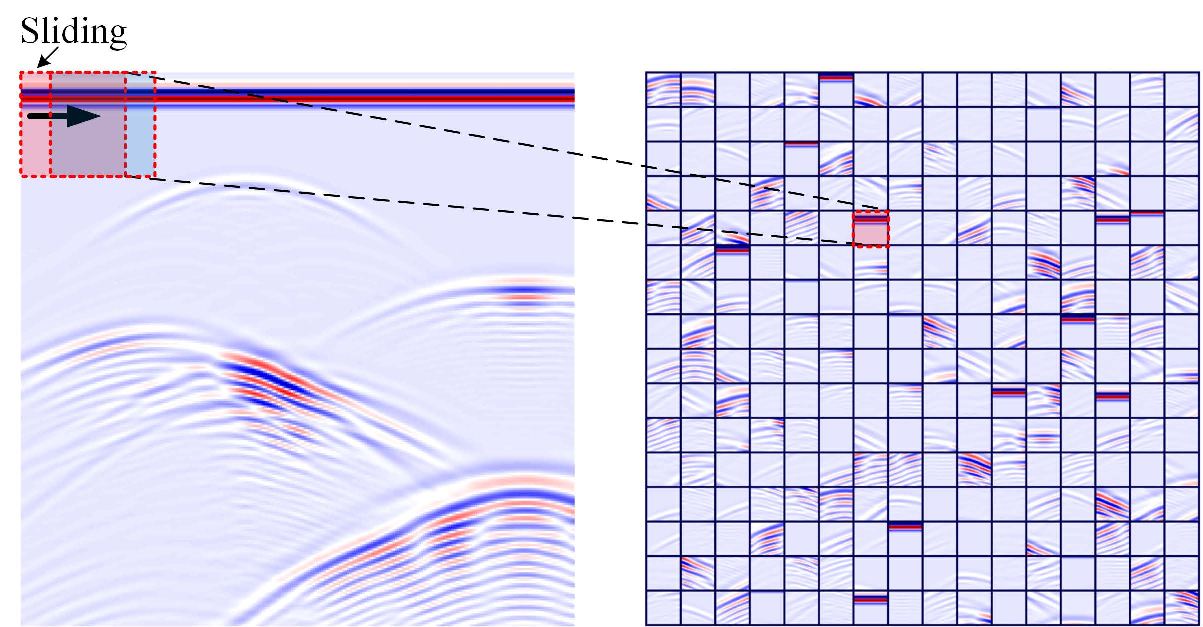
\includegraphics[width=3in]{./FigureFolder/Foundation/CDAEs/How2GetPatch.pdf}
\caption{块滑动方法制作数据集}
\label{Fig_How2GetPatch}
\end{figure}
\par
由于地球物理数据的特殊性,因此对传统的CDAEs网络结构进行了大量的调整,优化后的网络结构如图\ref{Fig_ConstructionOfResCDAEs}所示。
\begin{figure}[htbp]
\centering
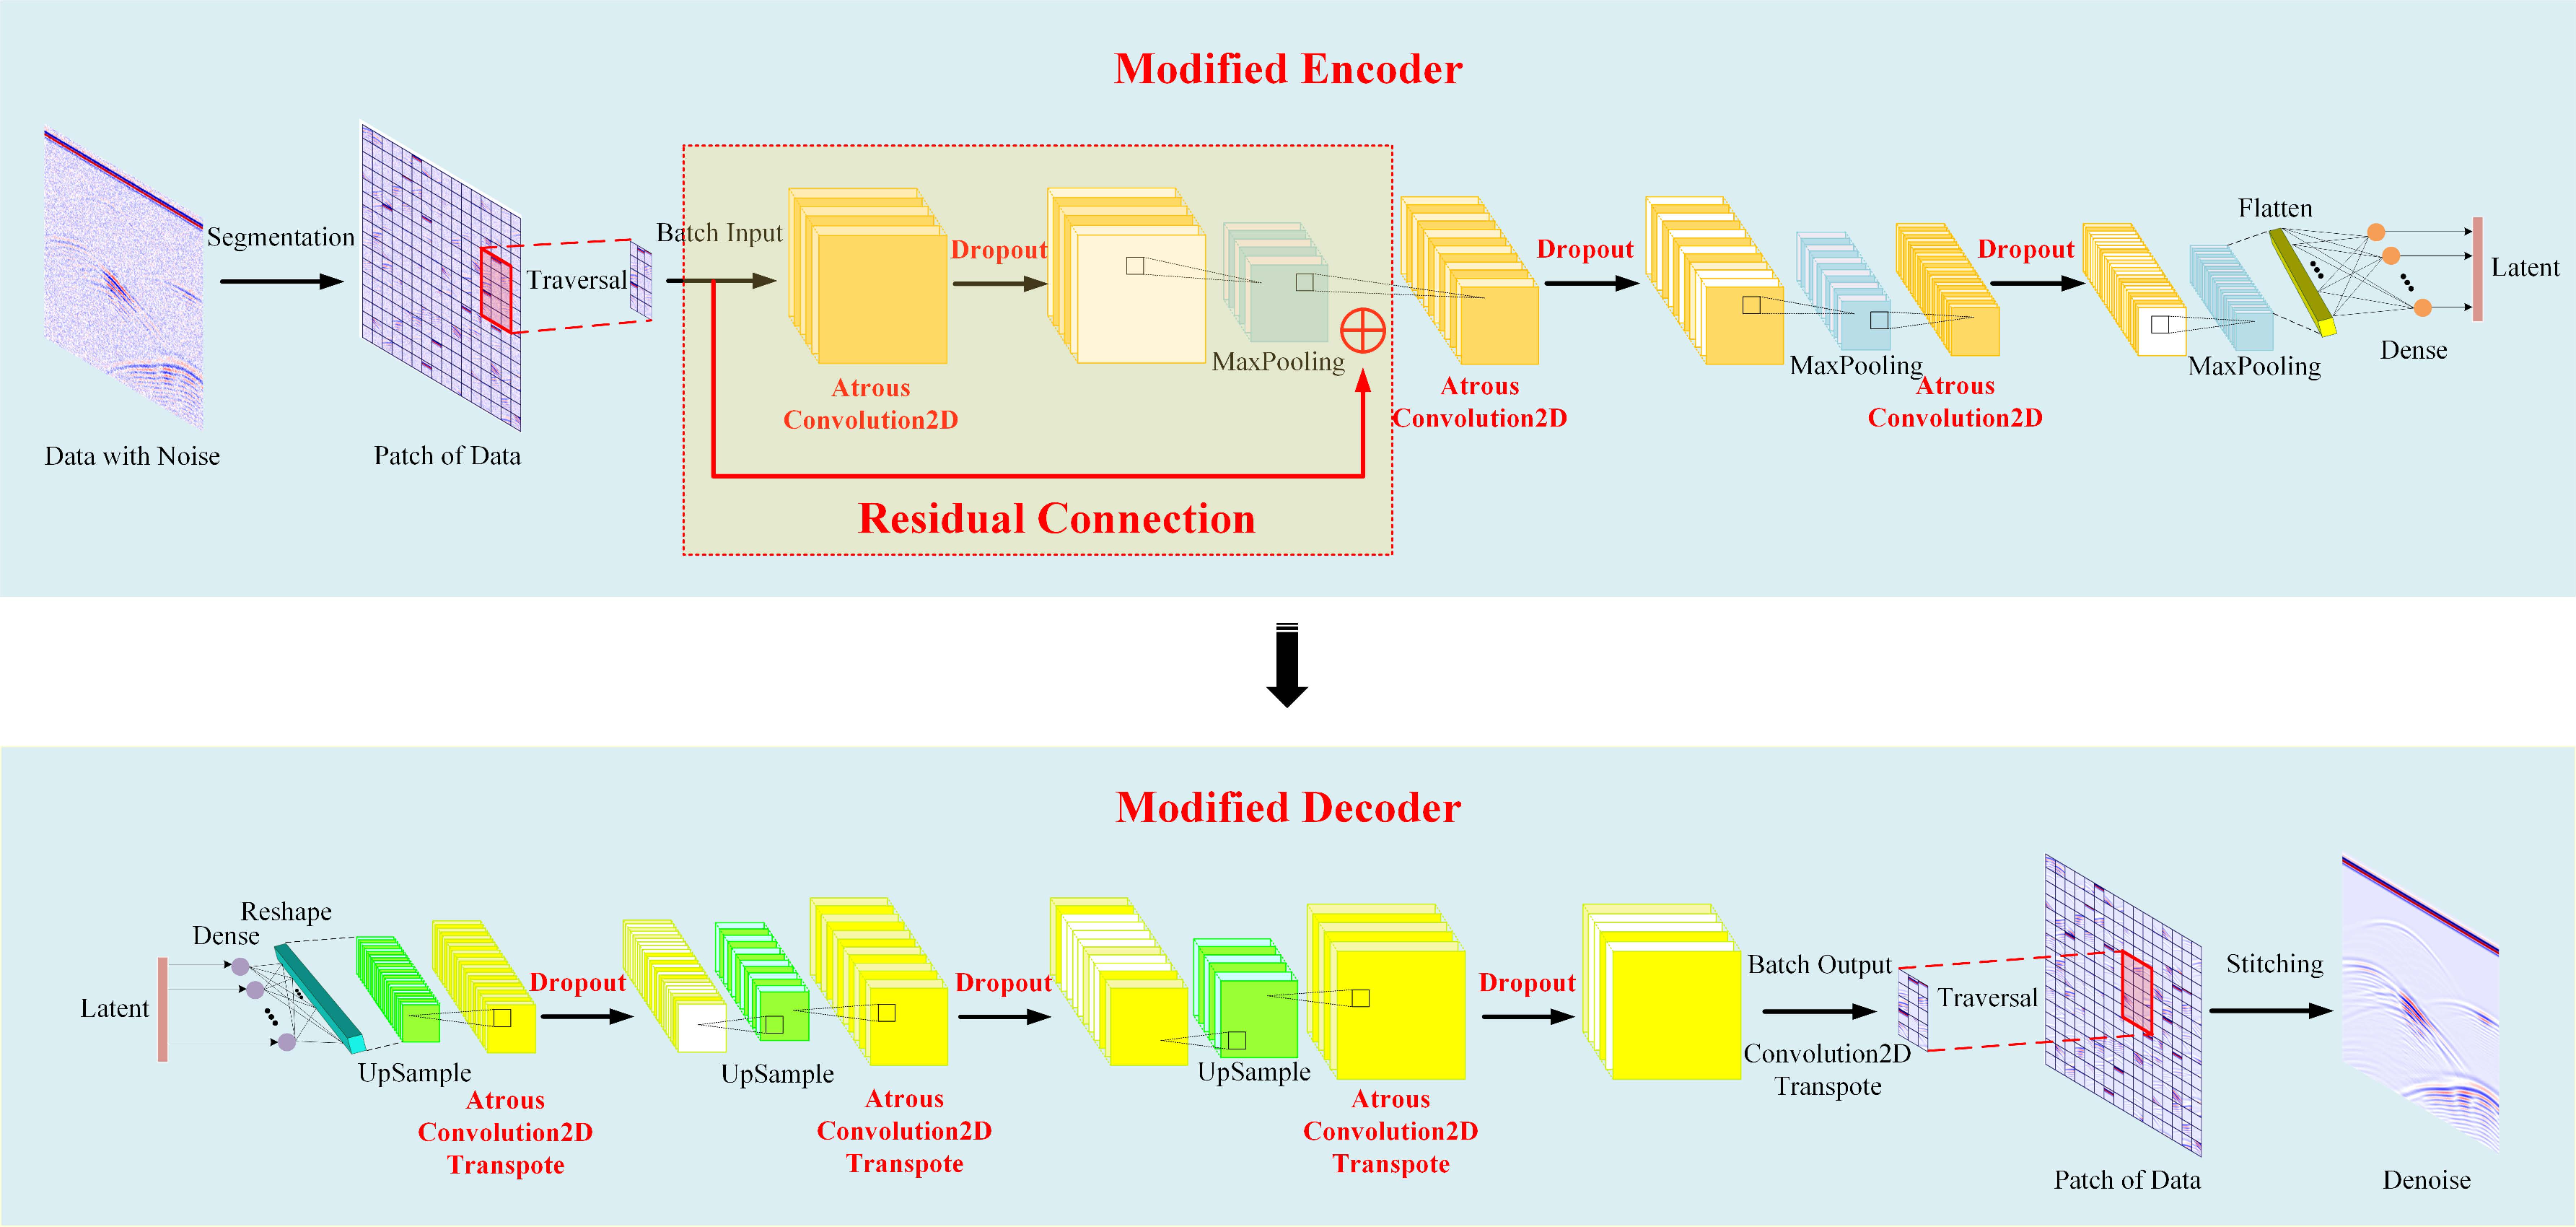
\includegraphics[width=5.5in]{./FigureFolder/Foundation/CDAEs/ConstructionOfResCDAEs.pdf}
\caption{结构优化的CDAEs}
\label{Fig_ConstructionOfResCDAEs}
\end{figure}
\par
由图\ref{Fig_ConstructionOfResCDAEs}可见,为了解决GPR数据的冗余性,同时保证网络结构的稳定性,防止梯度爆炸和梯度消失的现象,添加了Dropout正则化层、使用了Atrous卷积核、添加了Residual Connection等网络结构,保证了网络的稳定,提高了数据的保真性。
\par
对于合成复杂衬砌模型剖面数据的去噪结果如图\ref{Fig_Denoise}所示,图\ref{Fig_Denoise}(a)为无噪数据剖面,图\ref{Fig_Denoise}(b)为含噪数据剖面,图\ref{Fig_Denoise}(c)为使用结构优化的CDAEs的去噪结果剖面,图\ref{Fig_Denoise}(d)为去噪后的残差数据。
\begin{figure}[htbp]
\centering
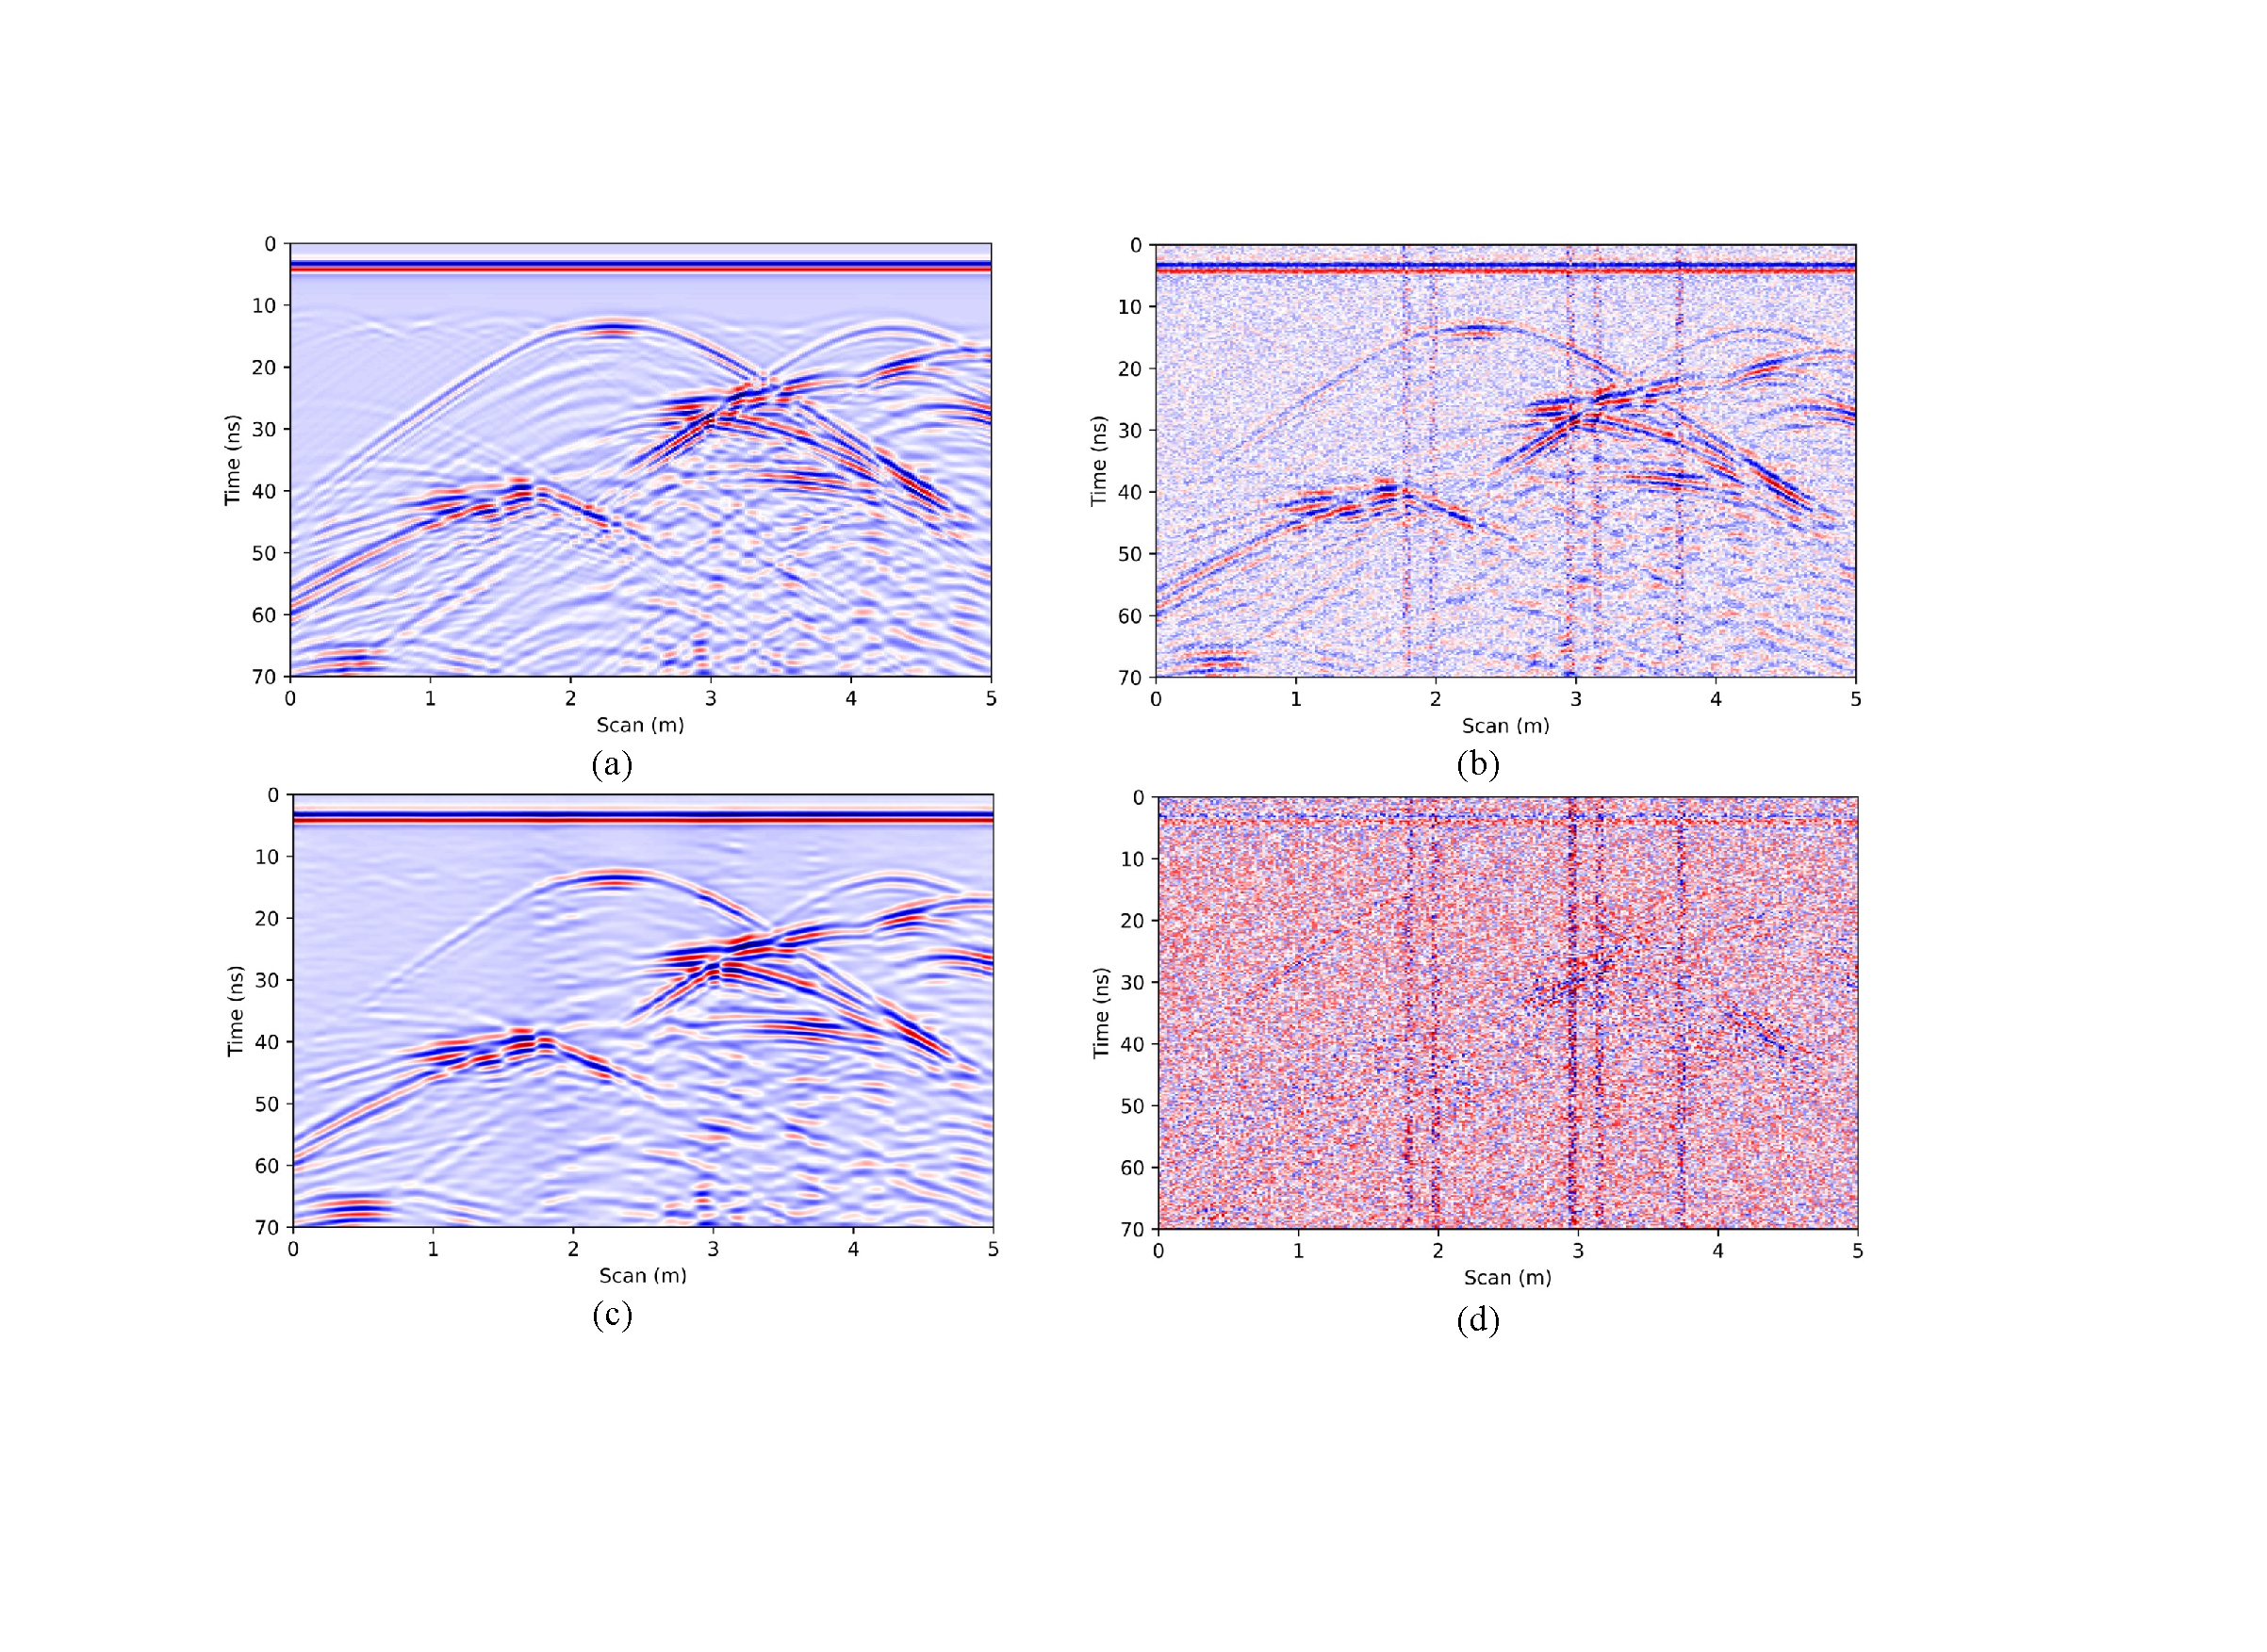
\includegraphics[width=3in]{./FigureFolder/Foundation/CDAEs/Denoise.pdf}
\caption{合成数据去噪结果}
\label{Fig_Denoise}
\end{figure}
\par
从合成数据的去噪结果中可以看出,结构优化的CDAEs针对高斯白噪声和高斯尖锐脉冲噪声具有良好的适应性,并且对原始数据的损失很少,达到了高保真去噪的目的。
\par
为了说明结构优化的CDAEs对实测模型的适用性,选取了一组实测数据,去噪结果如图\ref{Fig_DenoiseWiggle}所示,其中图\ref{Fig_DenoiseWiggle}(a)为原始剖面数据,图\ref{Fig_DenoiseWiggle}(b)为使用CDAEs得到的去噪结果剖面数据,图\ref{Fig_DenoiseWiggle}(c)为去噪后的残差数据。
\begin{figure}[htbp]
\centering
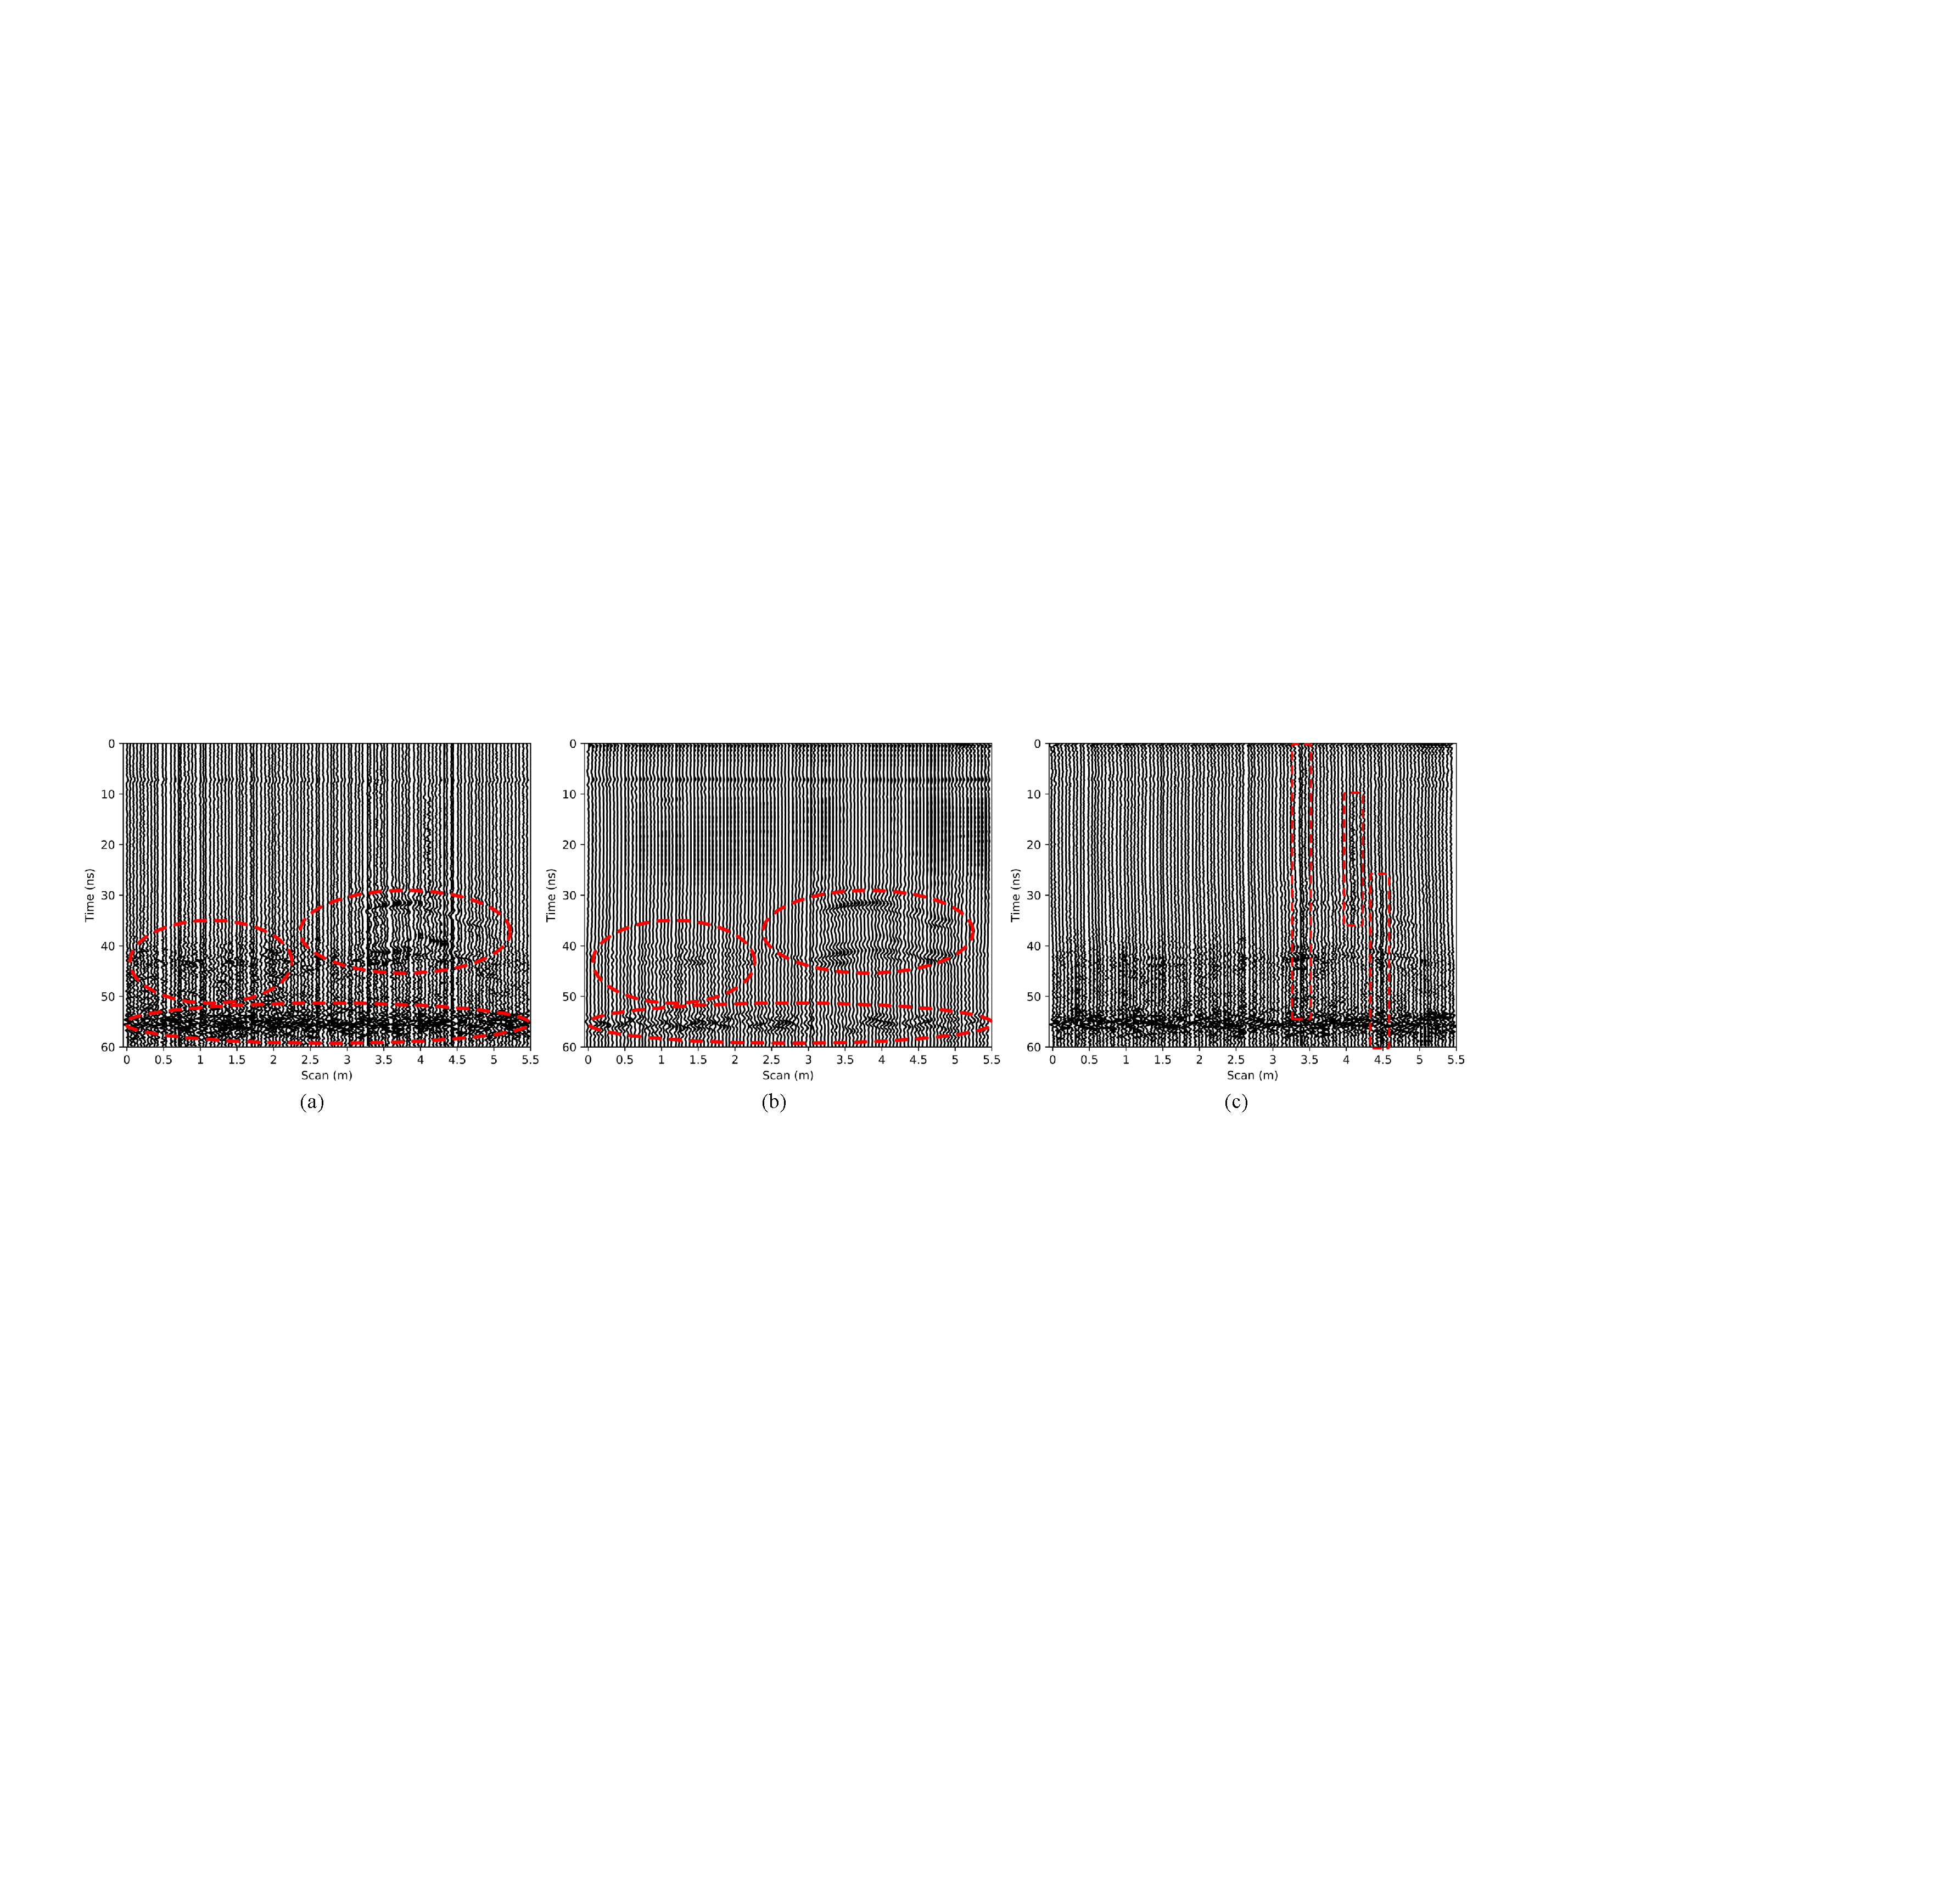
\includegraphics[width=5.5in]{./FigureFolder/Foundation/CDAEs/DenoiseWiggle.pdf}
\caption{实测数据去噪结果}
\label{Fig_DenoiseWiggle}
\end{figure}
\par
从实测数据的去噪结果中可以看出,结构优化的CDAEs不仅在合成数据上表现良好,并且在实测数据上依然具有良好的适应性,图\ref{Fig_DenoiseWiggle}中原始数据中的高斯噪声、高斯尖锐脉冲信号和地下杂乱波形等得到较好的去除,异常体得到了更加明显的突出。
\par
对于GPR剖面数据的去噪处理至此全部完成,以上过程的详细代码及数据已发布至$https://github.com/nephilim2016/AutoEncoder-for-GPR-Denoise$。

\subsection*{\kai\fontsize{11pt}{10pt} \selectfont【声波方程全波形反演】}
为了对比不同的正则化模型约束方法的效果,建立一个双``十''字型模型,设置四组双参数反演实验,(a) Tikhonov正则化模型约束;(b) 采用自适应全变差正则化因子策略的传统全变差正则化模型约束;(c) 采用自适应全变差正则化因子策略的修正全变差正则化模型约束;(d) 采用自适应全变差正则化因子策略的考虑高阶项的修正全变差正则化模型约束。图\ref{Fig_CrossModel}为四组不同正则化模型约束方法下的介质速度反演剖面图,依次
为(a)Tikhonov正则化模型约束、(b)传统全变差正则化模型约束、(c)改进全变差正则化模型约束策略、(d) 采用自适应全变差正则化因子策略的考虑高阶项的修正全变差正则化模型约束策略。
\begin{figure}[htbp]
\centering
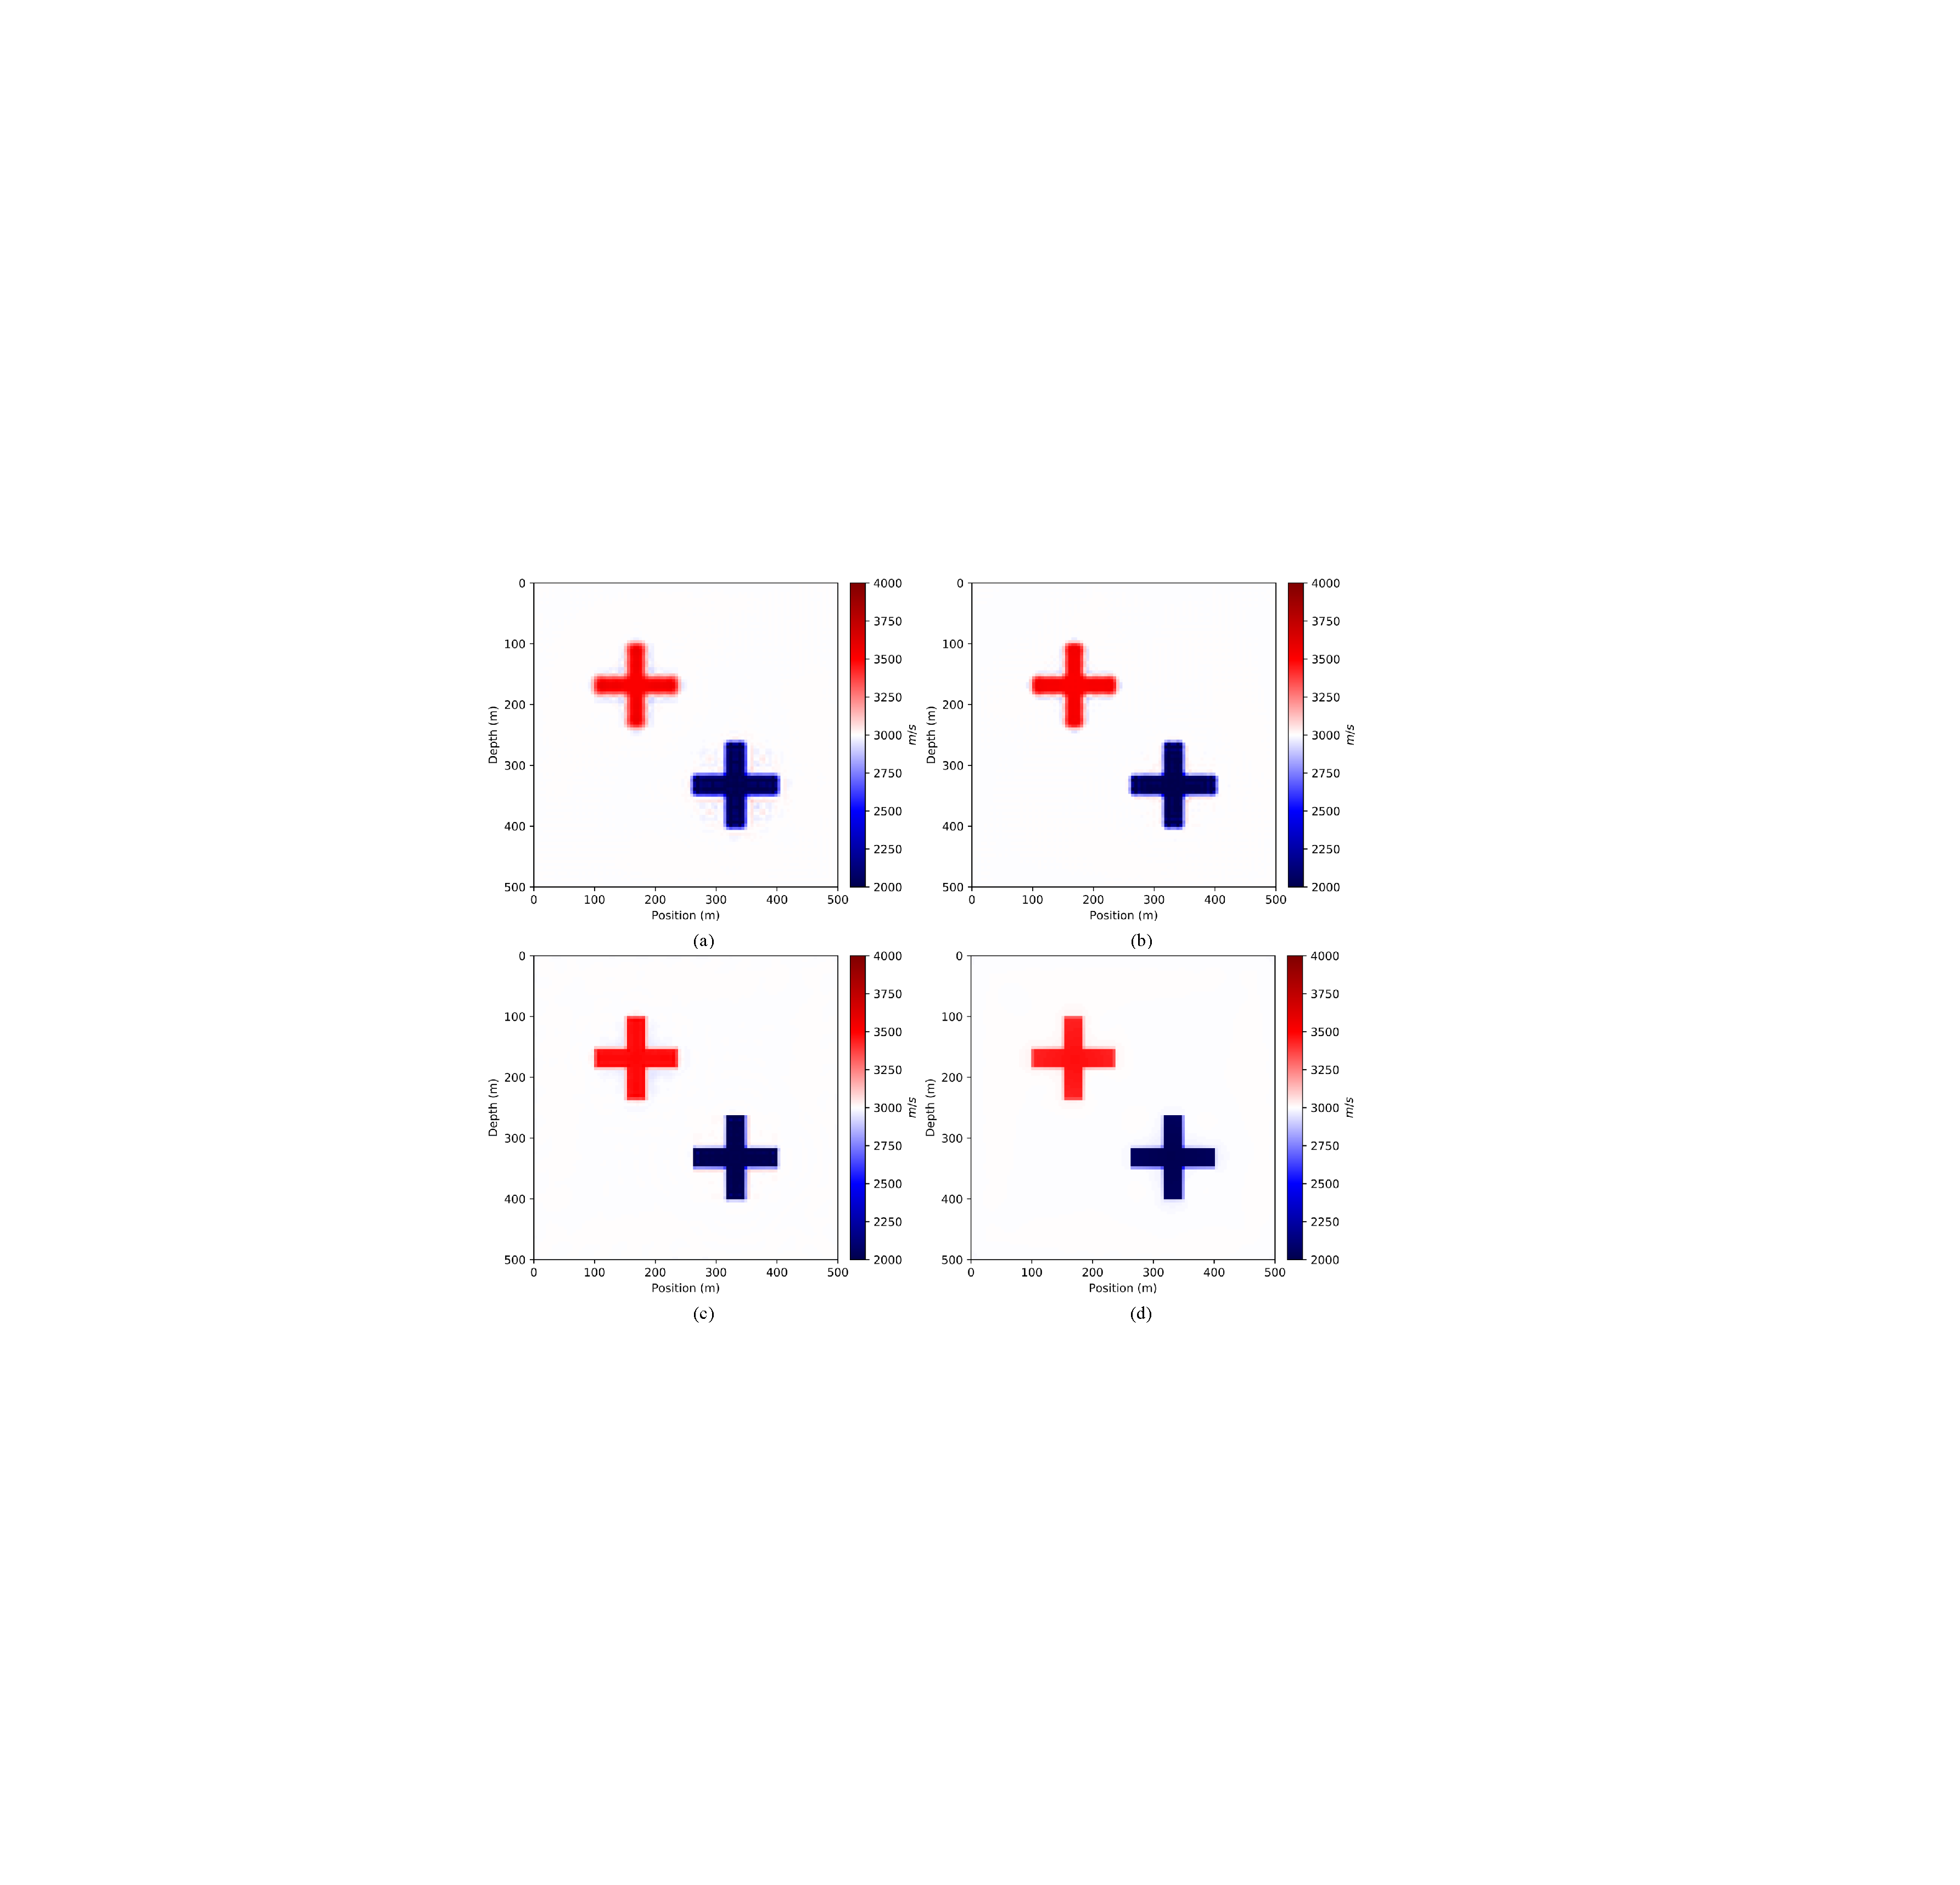
\includegraphics[width=3in]{./FigureFolder/Foundation/FWI/CrossModel.pdf}
\caption{不同正则化策略全波形反演对比图}
\label{Fig_CrossModel}
\end{figure}
\par
综合对比四幅反演结果图可知,(a)策略加载了Tikhonov正则化模型约束,可以发现相较于不加载正则化模型约束的全波形反演结果,Tikhonov正则化模型约束并没有提高反演图像的清晰度,异常体分界面模糊且存在非物理震荡现象,这是由于Tikhonov正则化模型约束会使异常体分界面过度平滑导致的;(b)策略通过加载传统的全变差正则化方法,一定程度上改善了反演图像的清晰度,提高了异常体分界面的分辨率,降低了背景的非物理震荡现象,然而由于平滑参数的存在,使得异常体分界面比较平滑,没有很好地突出分界面的位置;(c)策略、(d)策略全波形反演结果相似,仅从重构结果上看反演图像最清晰,异常体分界面最为明显,背景几乎不存在非物理震荡,异常体重构效果最好。综上所述,通过加载一个使用自适应的正则化因子的正则化模型约束,使数据拟合与模型约束之间达到更好的平衡,在一定程度上确实可以压制背景的非物理振荡,提高反演剖面的分辨率,使得分界面更加明显。
\par
为了更好地对比四种不同反演策略下的反演结果并且直观反映修正全变差正则化模型约束及考虑高阶项的修正全变差正则化模型约束的反演细节,通过对比四组不同正则化模型约束方法下的单道切线剖面,如图\ref{Fig_CrossModelLine}所示。
\begin{figure}[htbp]
\centering
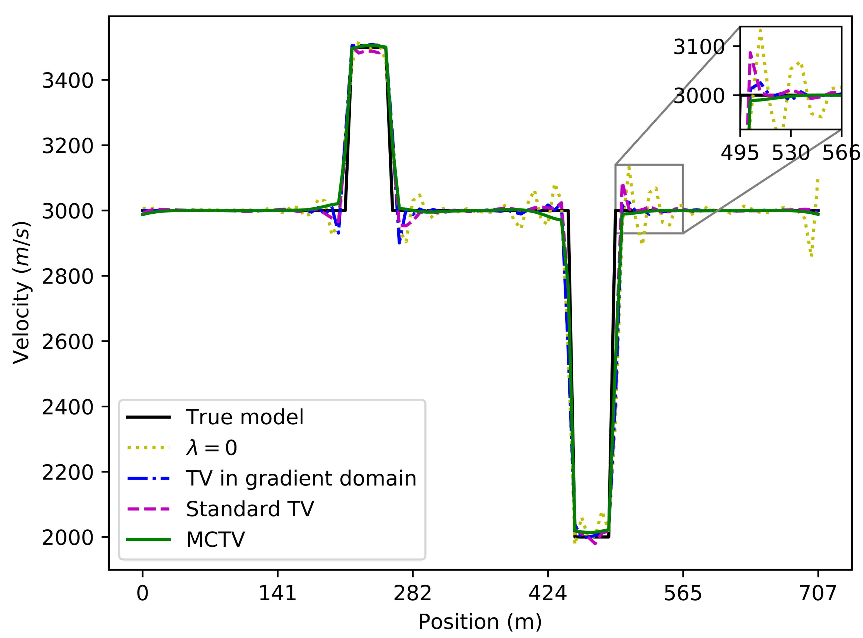
\includegraphics[width=3in]{./FigureFolder/Foundation/FWI/CrossModelLine.pdf}
\caption{不同正则化策略全波形反演对比图}
\label{Fig_CrossModelLine}
\end{figure}
\par
可以发现,黄色点线代表的加载Tikhonov正则化模型约束的反演结果存在较大的非物理震荡现象,异常体边界十分模糊,介质内部均一区域存在震荡现象;蓝色点划线代表的加载传统全变差正则化模型约束的反演结果在一定程度下降低了非物理震荡现象,提高了异常体分界面的分辨率,但降低了介质密度反演幅值的精确度,且没有改善介质内部均一区域存在的震荡现象;紫色虚线代表的加载修正全变差正则化模型约束的反演结果在不降低反演幅值精确度的同时,不仅有效地降低了非物理震荡现象,提高了异常体分界面的分辨率,而且减小了介质内部均一区域存在的震荡现象,但在异常体分界面处存在不可忽视的震荡现象;绿色实线代表的加载考虑高阶项的修正全变差正则化模型约束的反演结果在不降低反演幅值精确度的同时,不仅有效地降低了非物
理震荡现象,提高了异常体分界面的分辨率,而且消除了介质内部均一区域和异常体分界面处存在的振荡现象,且在分界面的细节部分更加接近真实模型,在细节方面较使用修正全变差正则化模型约束策略具有更高的分辨率。
\par
为了提高全波形反演的效率,使用了动态随机震源编码地震全波形反演策略,该策略能够从多个方便综合压制炮间的串扰噪声,各种随机时域震源编码方法优势互补,共同作用极大地削弱了串扰噪声对全波形反演的影响,并且由于采用了动态策略,既避免了相同的独立震源导致的相同的串扰噪声作用在每次反演迭代中,从而进一步压制串扰噪声,又避免了随机相位震源编码造成深部信息缺失及随机振幅震源编码造成炮信息不对称的问题,并对受串扰噪声干扰的部分加以修正,从而大幅提高全波形反演的精度。
\par
为了进一步提高全波形反演的精度,因此将两种反演结合起来,形成了基于MCTV正则化的动态随机震源编码地震全波形反演策略,选用BP1994地震标准模型为例,得到的反演结果如图\ref{Fig_BP1994Model}所示。
\begin{figure}[htbp]
\centering
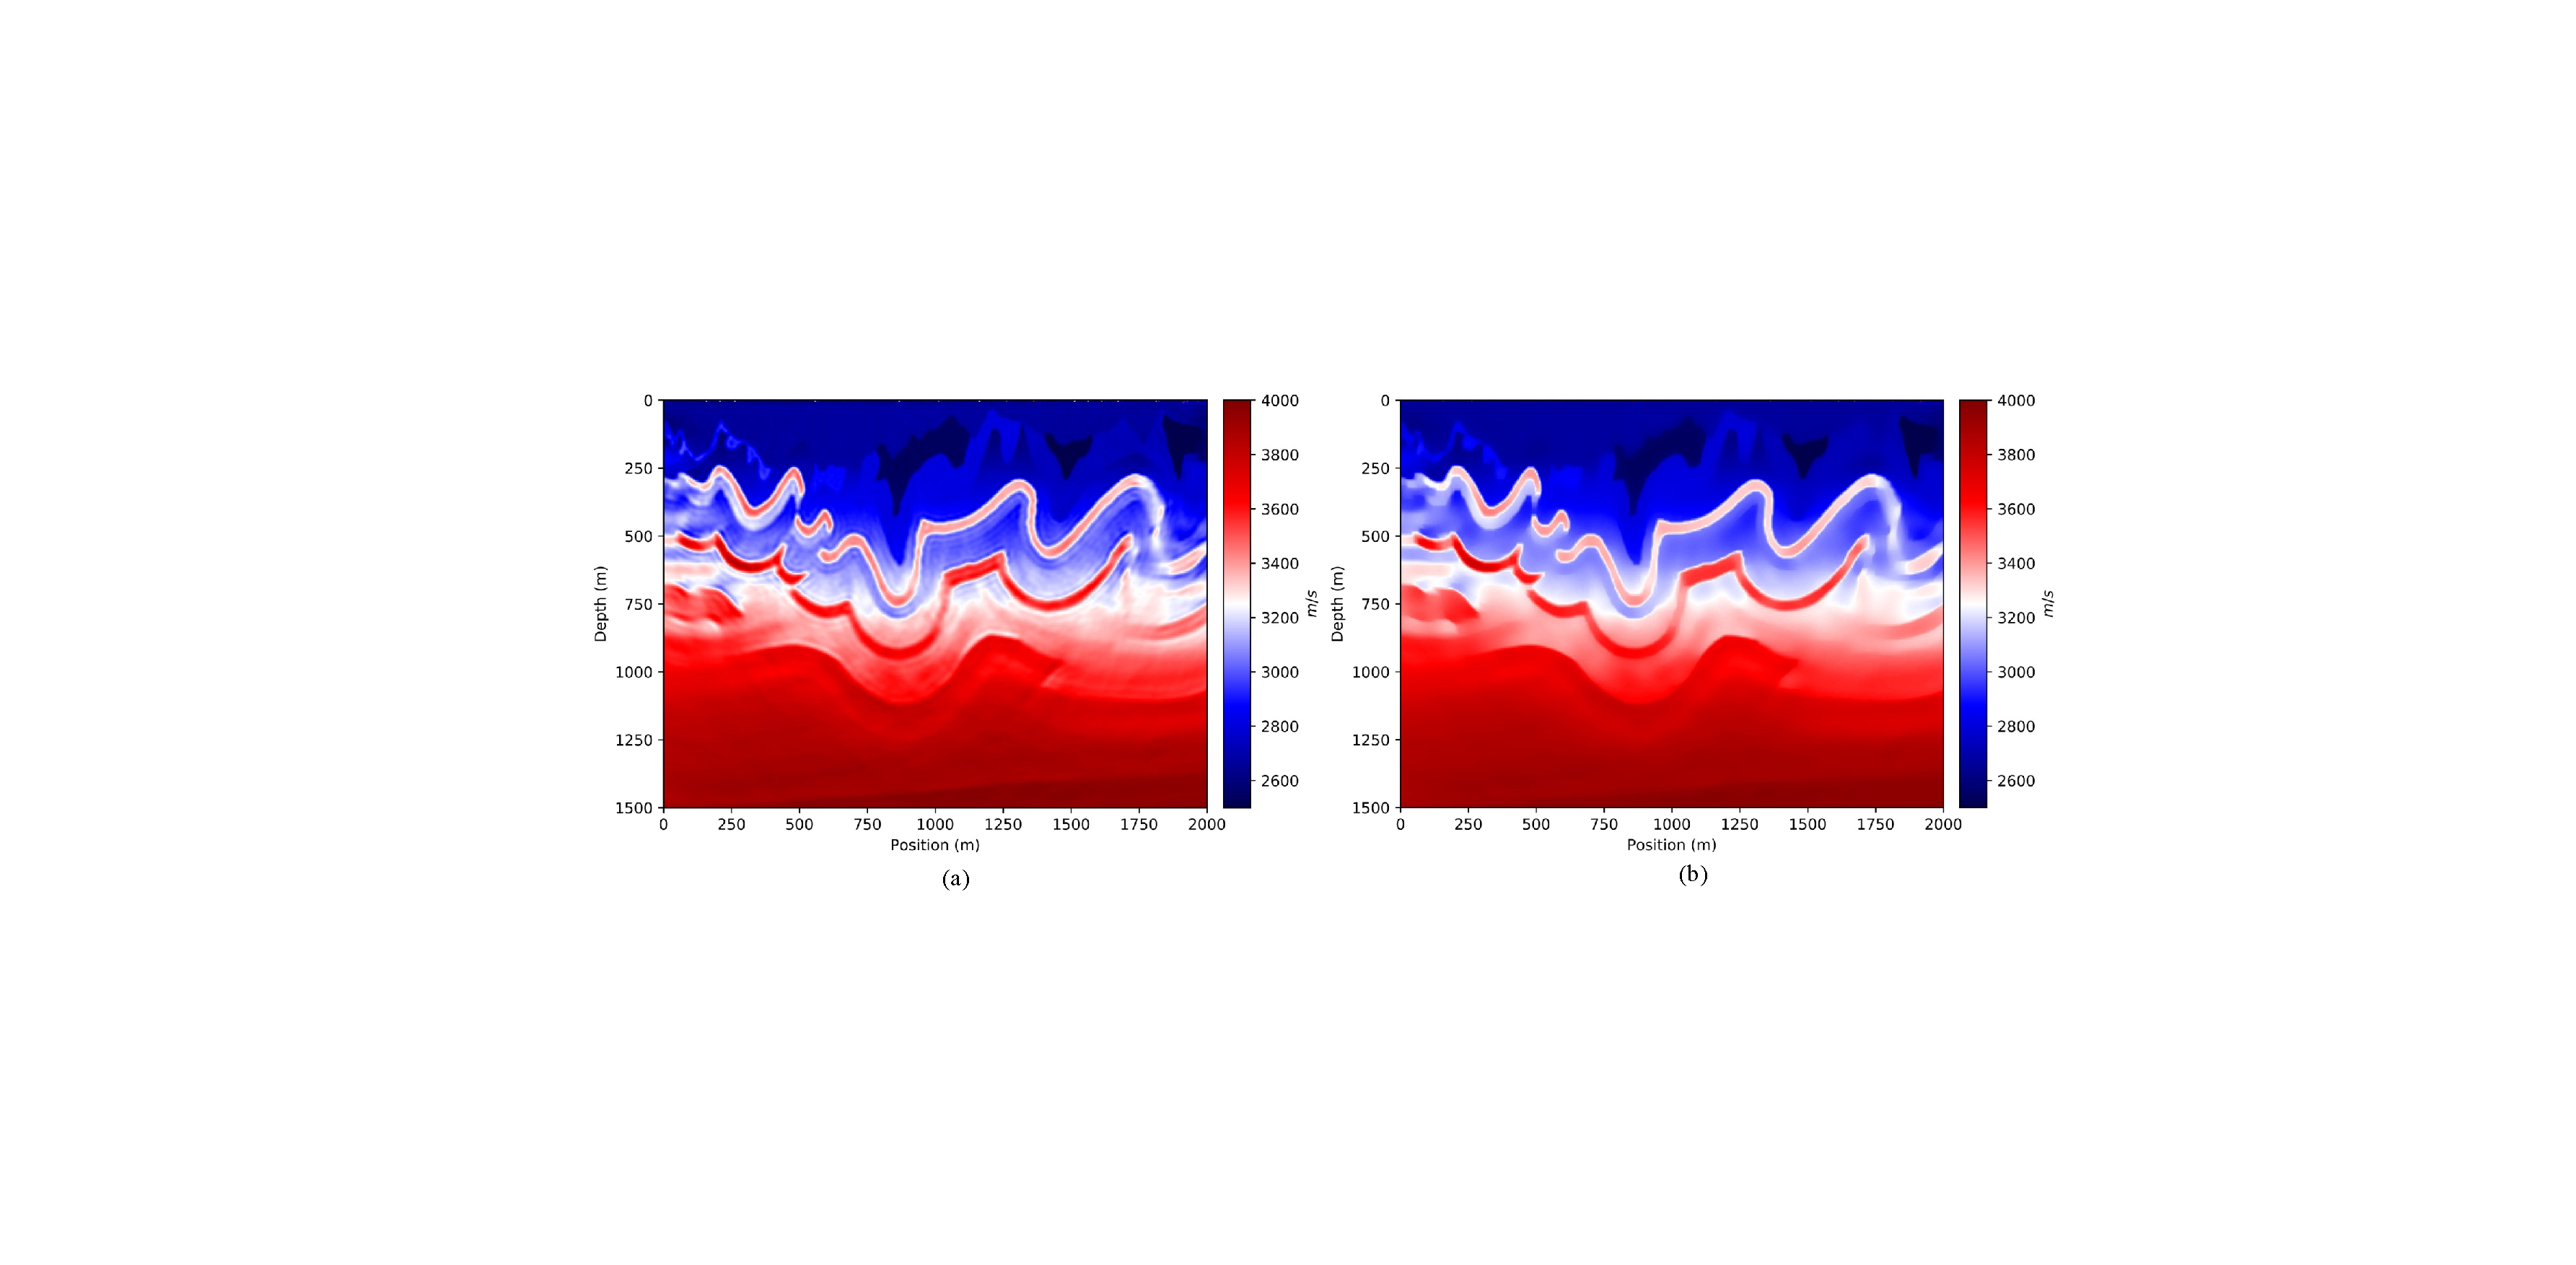
\includegraphics[width=5.5in]{./FigureFolder/Foundation/FWI/BP1994Model.pdf}
\caption{基于MCTV正则化的动态随机震源编码地震全波形反演结果}
\label{Fig_BP1994Model}
\end{figure}
\par
图\ref{Fig_BP1994Model}(a)为动态随机震源编码地震全波形反演结果,从结果上来看,反演结果与原始模型大致相似,但是细节方面仍然存在串扰噪声,图\ref{Fig_BP1994Model}(b)为基于MCTV正则化的动态随机震源编码地震全波形反演结果,对比来看,添加了MCTV正则化后在全波形反演精度上具有较大的提升。
\par
以上为全波形反演的研究的具体进展,以上过程的详细代码及数据已发布至$https://github.com/NephilimTeam/AcousticFWI_StochasticSourceEncoding$。
\subsection*{\kai\fontsize{11pt}{10pt} \selectfont【压缩感知】}
字典学习方法根据待处理数据中的信号结构特征自适应构建字典,突破了传统方法的固定基函数表达方式,字典中的一列被称为原子,相比较于传统的稀疏表示方法,字典中原子含有更加丰富的数据特征,能够更好地匹配信号本身,拥有更优秀地稀疏表示能力。
\par
在信号处理和图像处理领域提出的字典学习方法对于稀疏表示的发展起到了非常积极的推进作用,最早的字典学习算法是Sparsent字典学习算法,该算法利用最大似然估计方法训练字典,在自然图库中抽取大量的小图像作为字典,后来的改进算法多是使用梯度下降求解对应的优化问题,来提高其算法的收敛性。收到聚类算法的启发,Engan等人提出了最优方向(MOD)字典学习算法,使用l0范数求解信号的稀疏表示,并且利用交替优化来衡量学习模型。但是该算法的计算过程中,有大量的矩阵求逆和乘法运算,对电脑的计算能力与存储空间要求极高,难以推广。由Aharon首次提出了具有自适应性的超完备冗余字典K-SVD字典算法进行图像的稀疏分解,其与MOD算法的不同的是字典更新时,每次更新一列字典,而不是整个字典全部更新。基于超完备字典,对于数据不断地学习和训练,可以自适应地计算出最适合目标数据的字典,从而对目标数据进行稀疏表达。该方法再图像重构方面有着良好的效果,并且取得了广泛的应用。
\par
信号稀疏表示的两大主要任务就是字典的生成和信号的稀疏分解算法有匹配追踪算法、正交匹配追踪算法等。将稀疏分解理论应用到图像稀疏表示问题上,分别构造DCT过完备字典以及超完备冗余K-SVD字典。稀疏分解的过程主要是求取字典约束下的信号最佳稀疏表示形式,也可以看作是实现信号的稀疏表示。使用正交匹配追踪(Orthogonal Matching Pursuit,OMP)算法实现信号的稀疏分解。OMP算法是MP算法的一种改进,算法用Gram-Schmidt正交化将投影方向正交化来改进MP算法。
\par
DCT字典对周期信号有着良好的分解能力,DCT字典由离散余弦变换(Discrete Cosine Transform,DCT)获得,给定序号$x(n),n=0,1,\cdots,N-1$,其离散余弦变换为:
\begin{equation}\label{DCT_}
\begin{aligned}
x_c(0)&=\frac{1}{\sqrt{N}}\sum_{n=0}^{N-1} x(n)\\
x_c(k)&=\sqrt{\frac{2}{N}}\sum_{n=0}^{N-1} \cos \frac{(2n+1)k\pi}{2N}
\end{aligned}
\end{equation}
\par
如果写成矩阵形式,则有
\begin{equation}\label{DCTArray}
\mathbf{x}_c=\mathbf{c}_N \mathbf{x}
\end{equation}
\par
其中,$\mathbf{c}_N$为$N \times N$的变换矩阵,其行向量为余弦基。
\par
对于DCT变换后所得到的完备字典,采用分数频率法将其扩展成为过完备字典,具体的做法是将得到的完备字典对其频率上作更加精细的遍历和抽样,从而获得一个新的完备字典,一个过完备DCT字典如图\ref{Fig_DCT}所示。
\begin{figure}[htbp]
\centering
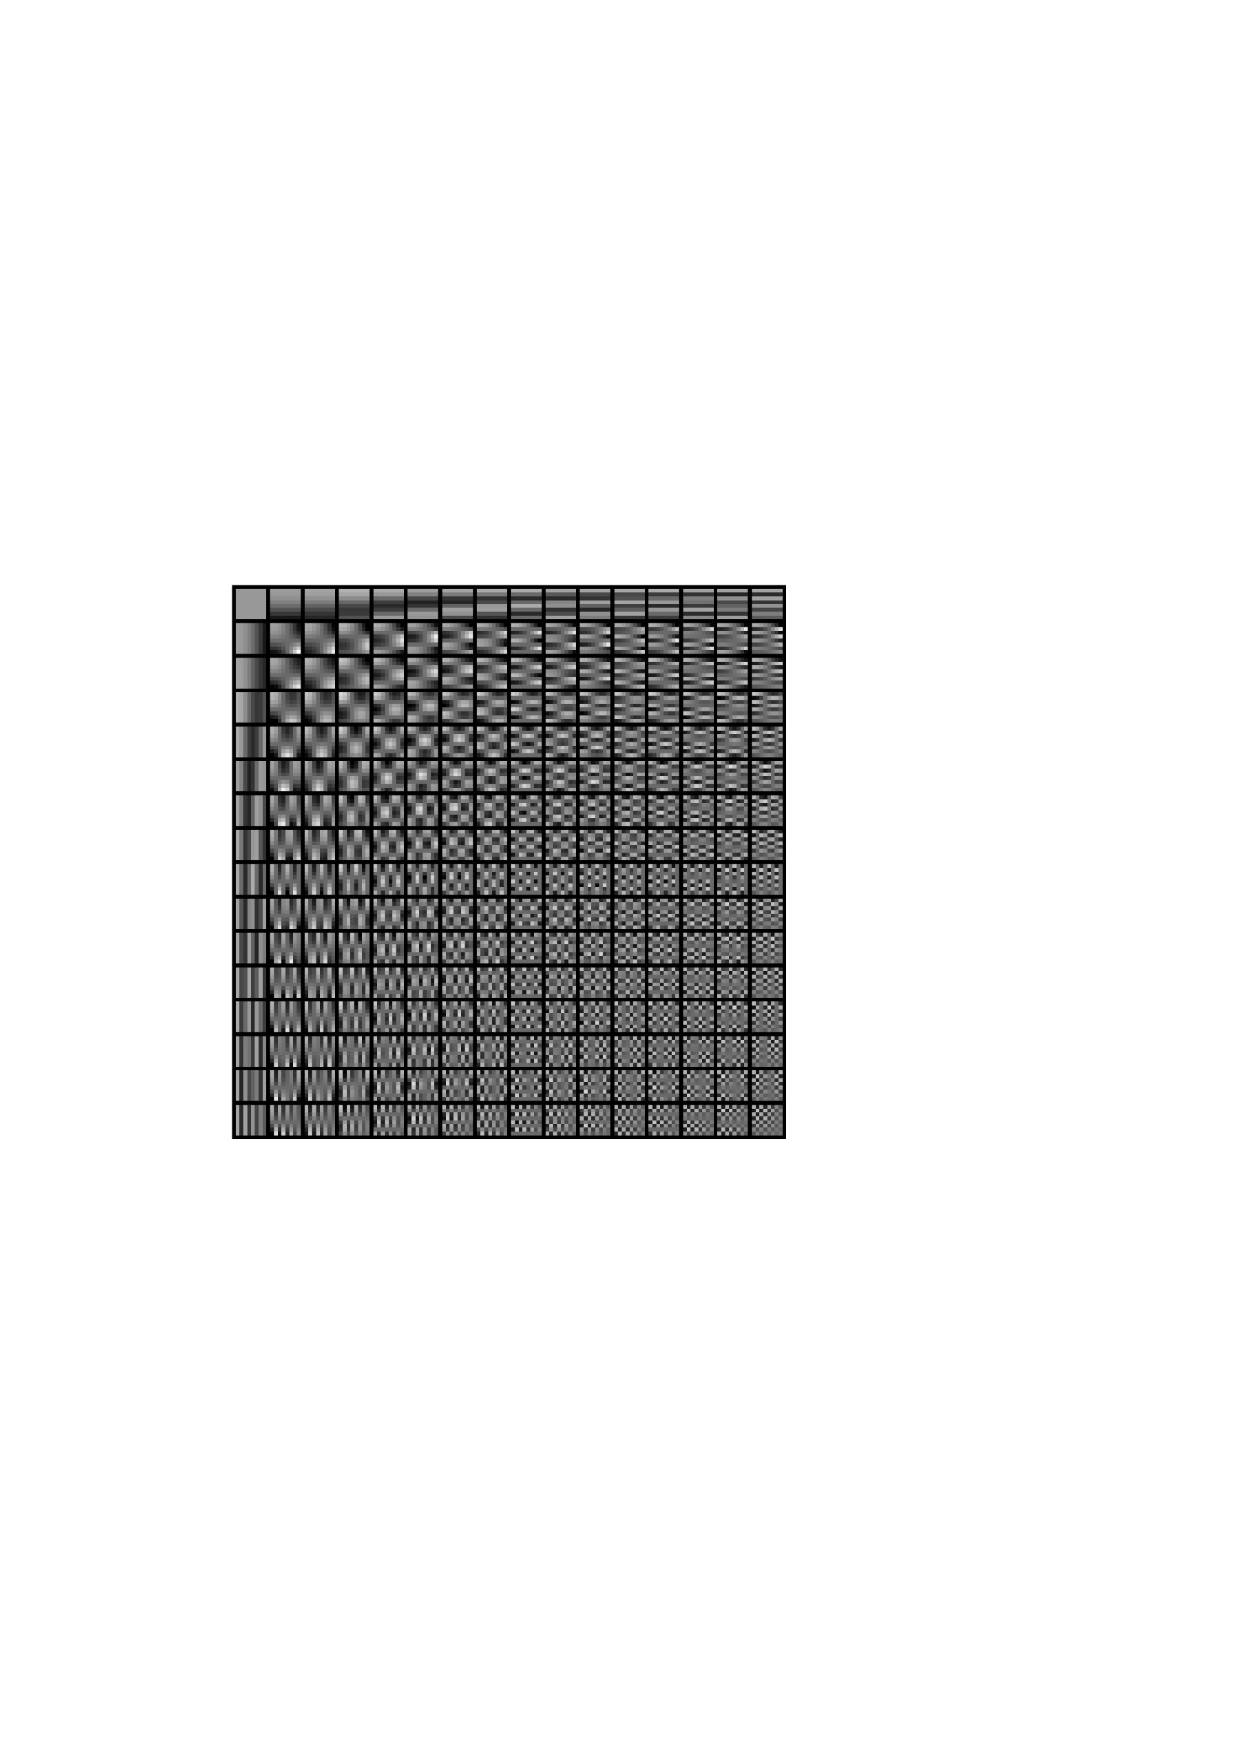
\includegraphics[width=2in]{./FigureFolder/Foundation/KSVD/DCT.pdf}
\caption{过完备DCT字典}
\label{Fig_DCT}
\end{figure}
\par
对于K-SVD字典,前文已有介绍,这里一个过完备K-SVD字典如图如图\ref{Fig_KSVD}所示。
\begin{figure}[htbp]
\centering
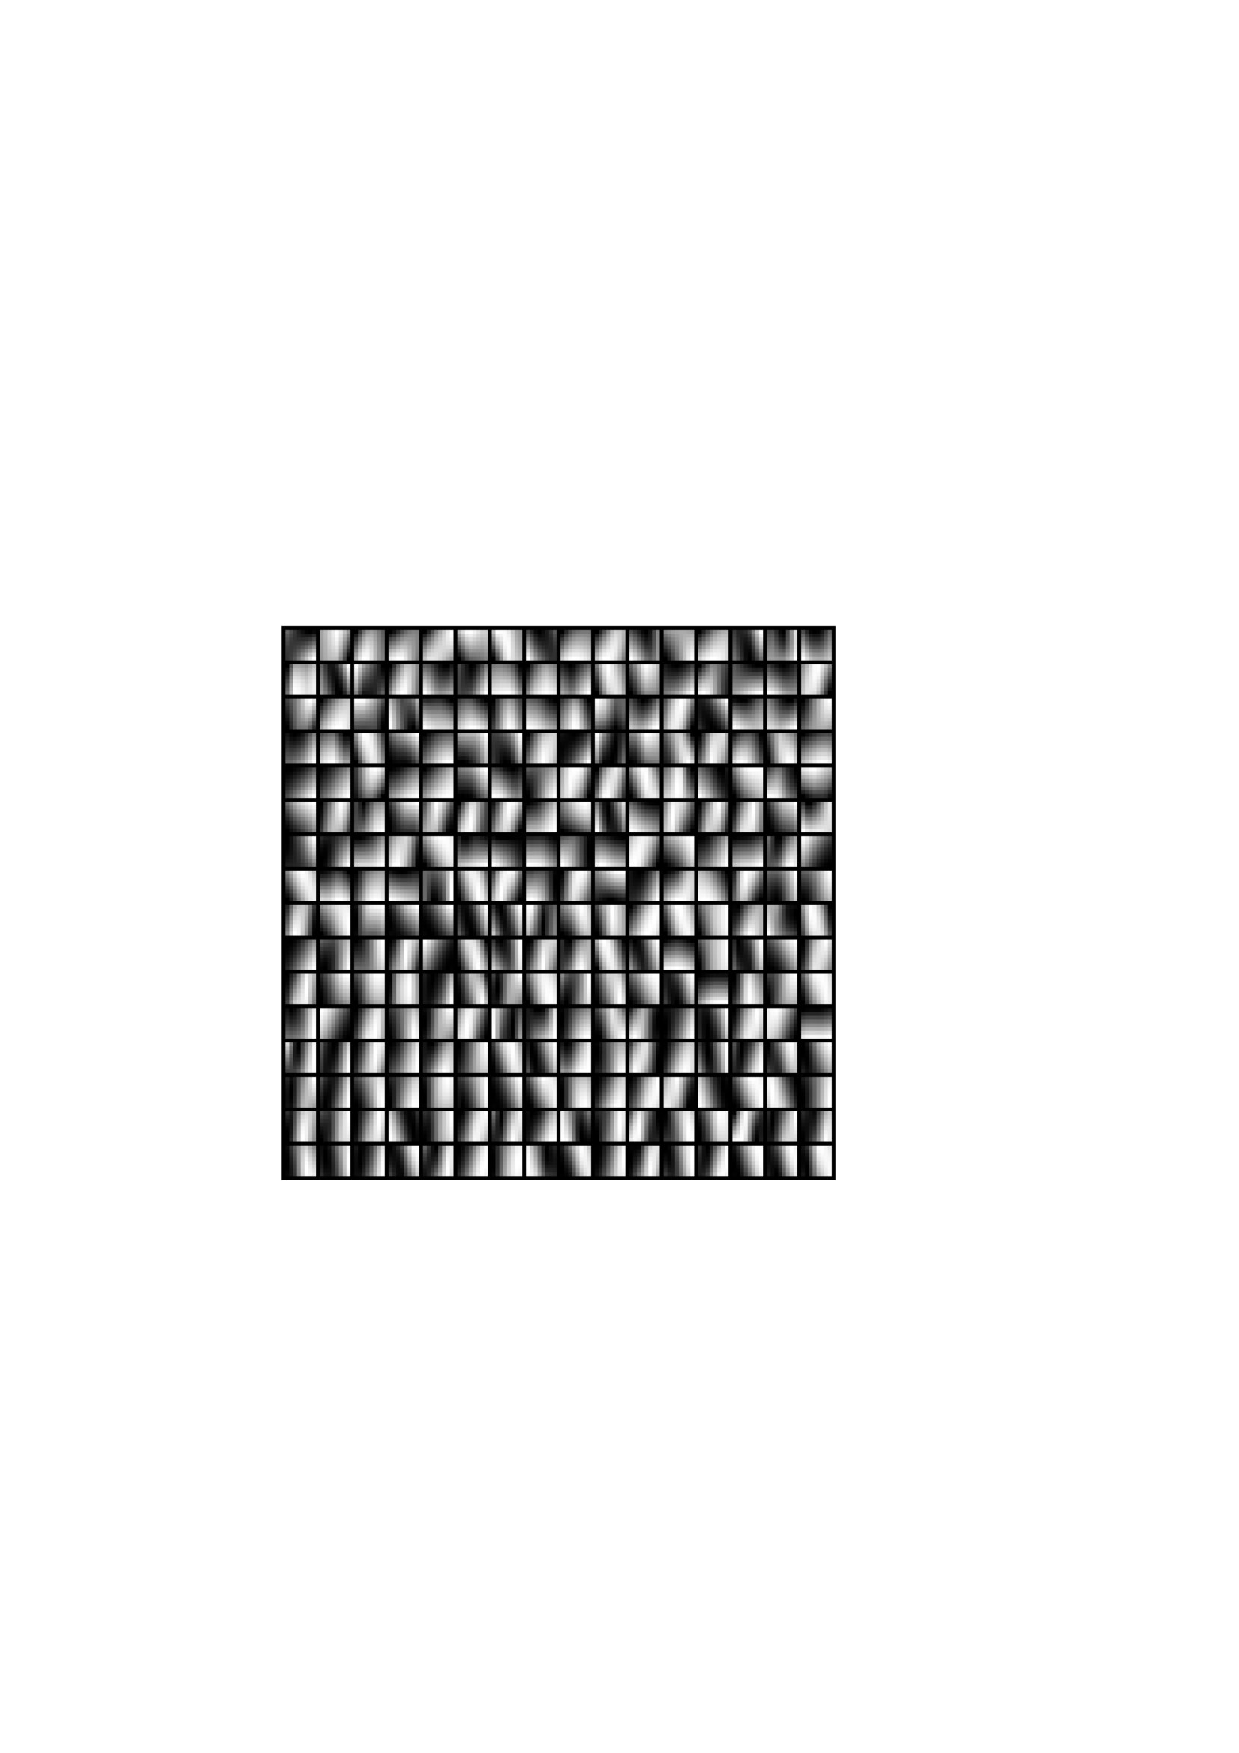
\includegraphics[width=2in]{./FigureFolder/Foundation/KSVD/KSVD.pdf}
\caption{过完备K-SVD字典}
\label{Fig_KSVD}
\end{figure}
\par
\subsection*{\kai\fontsize{11pt}{10pt} \selectfont【超分辨率网格映射】}
为了对比各种超分辨率策略对于网格映射的效果,使用$200 \times 400$的细网格数据,及$50 \times 100$的粗网格数据进行测试,数据使用Marmousi-ii国际标准模型,粗网格数据如图\ref{Fig_LR_Marmousi}所示,采用双三次插值映射到细网格的数据如图\ref{Fig_BC_Marmousi}所示。
\begin{figure}[htbp]
\centering
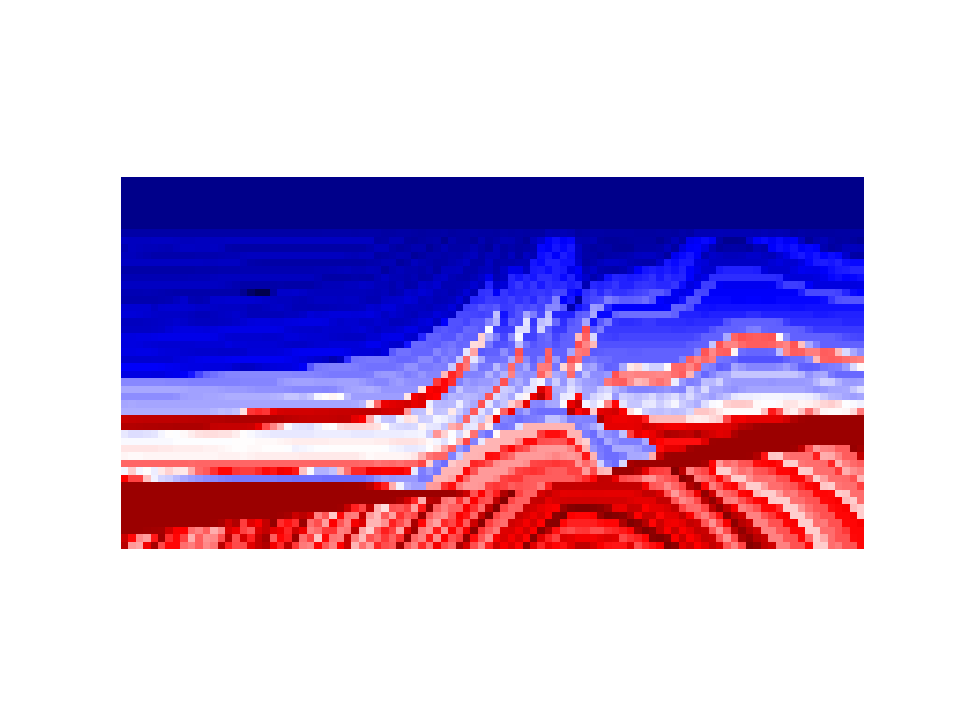
\includegraphics[width=3in]{./FigureFolder/Foundation/SuperResolution/SRCNN/LR_Marmousi.pdf}
\caption{粗网格Marmousi-ii模型数据}
\label{Fig_LR_Marmousi}
\end{figure}
\par
\begin{figure}[htbp]
\centering
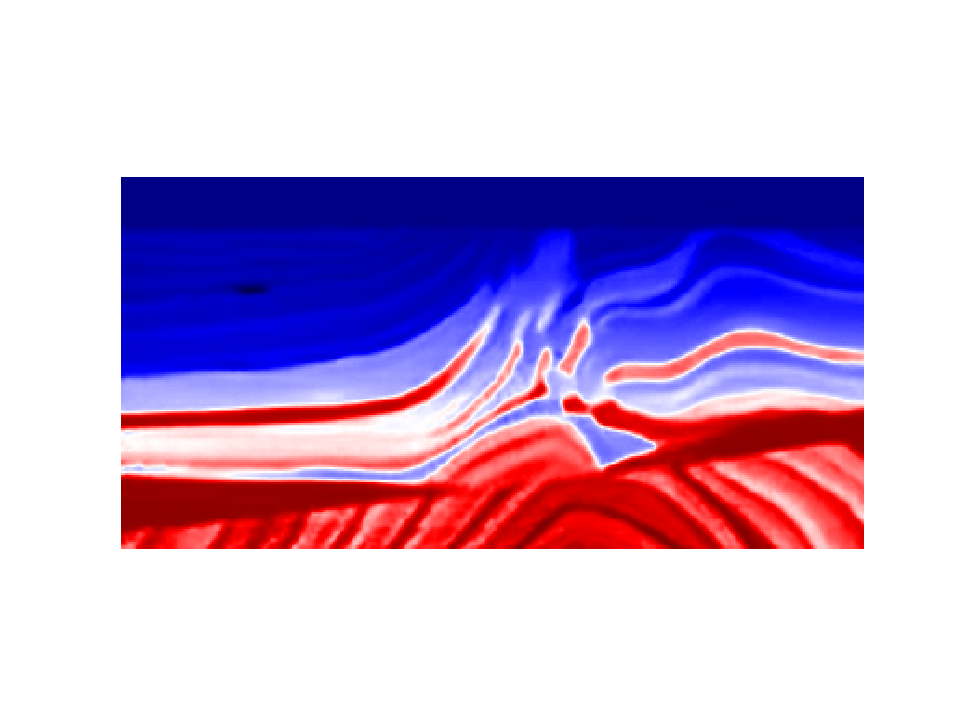
\includegraphics[width=3in]{./FigureFolder/Foundation/SuperResolution/SRCNN/BC_Marmousi.pdf}
\caption{Bicubic映射到细网格Marmousi-ii模型数据}
\label{Fig_BC_Marmousi}
\end{figure}
\par
从以上两图对比可以看出,粗网格数据较为粗糙,整体呈现锯齿状,使用双三次插值算法映射到细网格的数据虽然更加光滑,但是对于细节的信息表达较差,为了将评判标准量化,选取峰值信噪比(Peak Signal-to-Noise Ratio, PSRN)作为模型数据的评判标准,PSNR的计算公式为:
\par
\begin{equation}\label{PSNR}
PSNR=10 \cdot \log_{10} (\frac{MAX_I^2}{MSE})
\end{equation}
其中,$MSE=\frac{1}{mn}\sum_{i=0}^{m-1}\sum_{j=0}^{n-1} [ I(i,j)-K(i,j) ]^2$,这里$I$为原始数据,$K$为映射后的细网格数据,$m,n$分别为细网格大小,即$m \times n=200 \times 400$。计算得到双三次插值映射后的细网格数据$PSNR=24.0582dB$。
\par
1) SRCNN的实现
\par
SRCNN是FCNN在超分辨率中的初步应用之一,在SRCNN中,首先使用双三次插值对图像进行上采样,然后馈入简单的FCNN。重要的是要注意,不涉及池化操作。因此,导致输出具有与上采样的输入图像相同的空间尺寸的输出。最后,我们计算目标HR图像与输出之间的MSE损失。SRCNN网络结构如图\ref{Fig_SRCNN}所示。
\begin{figure}[htbp]
\centering
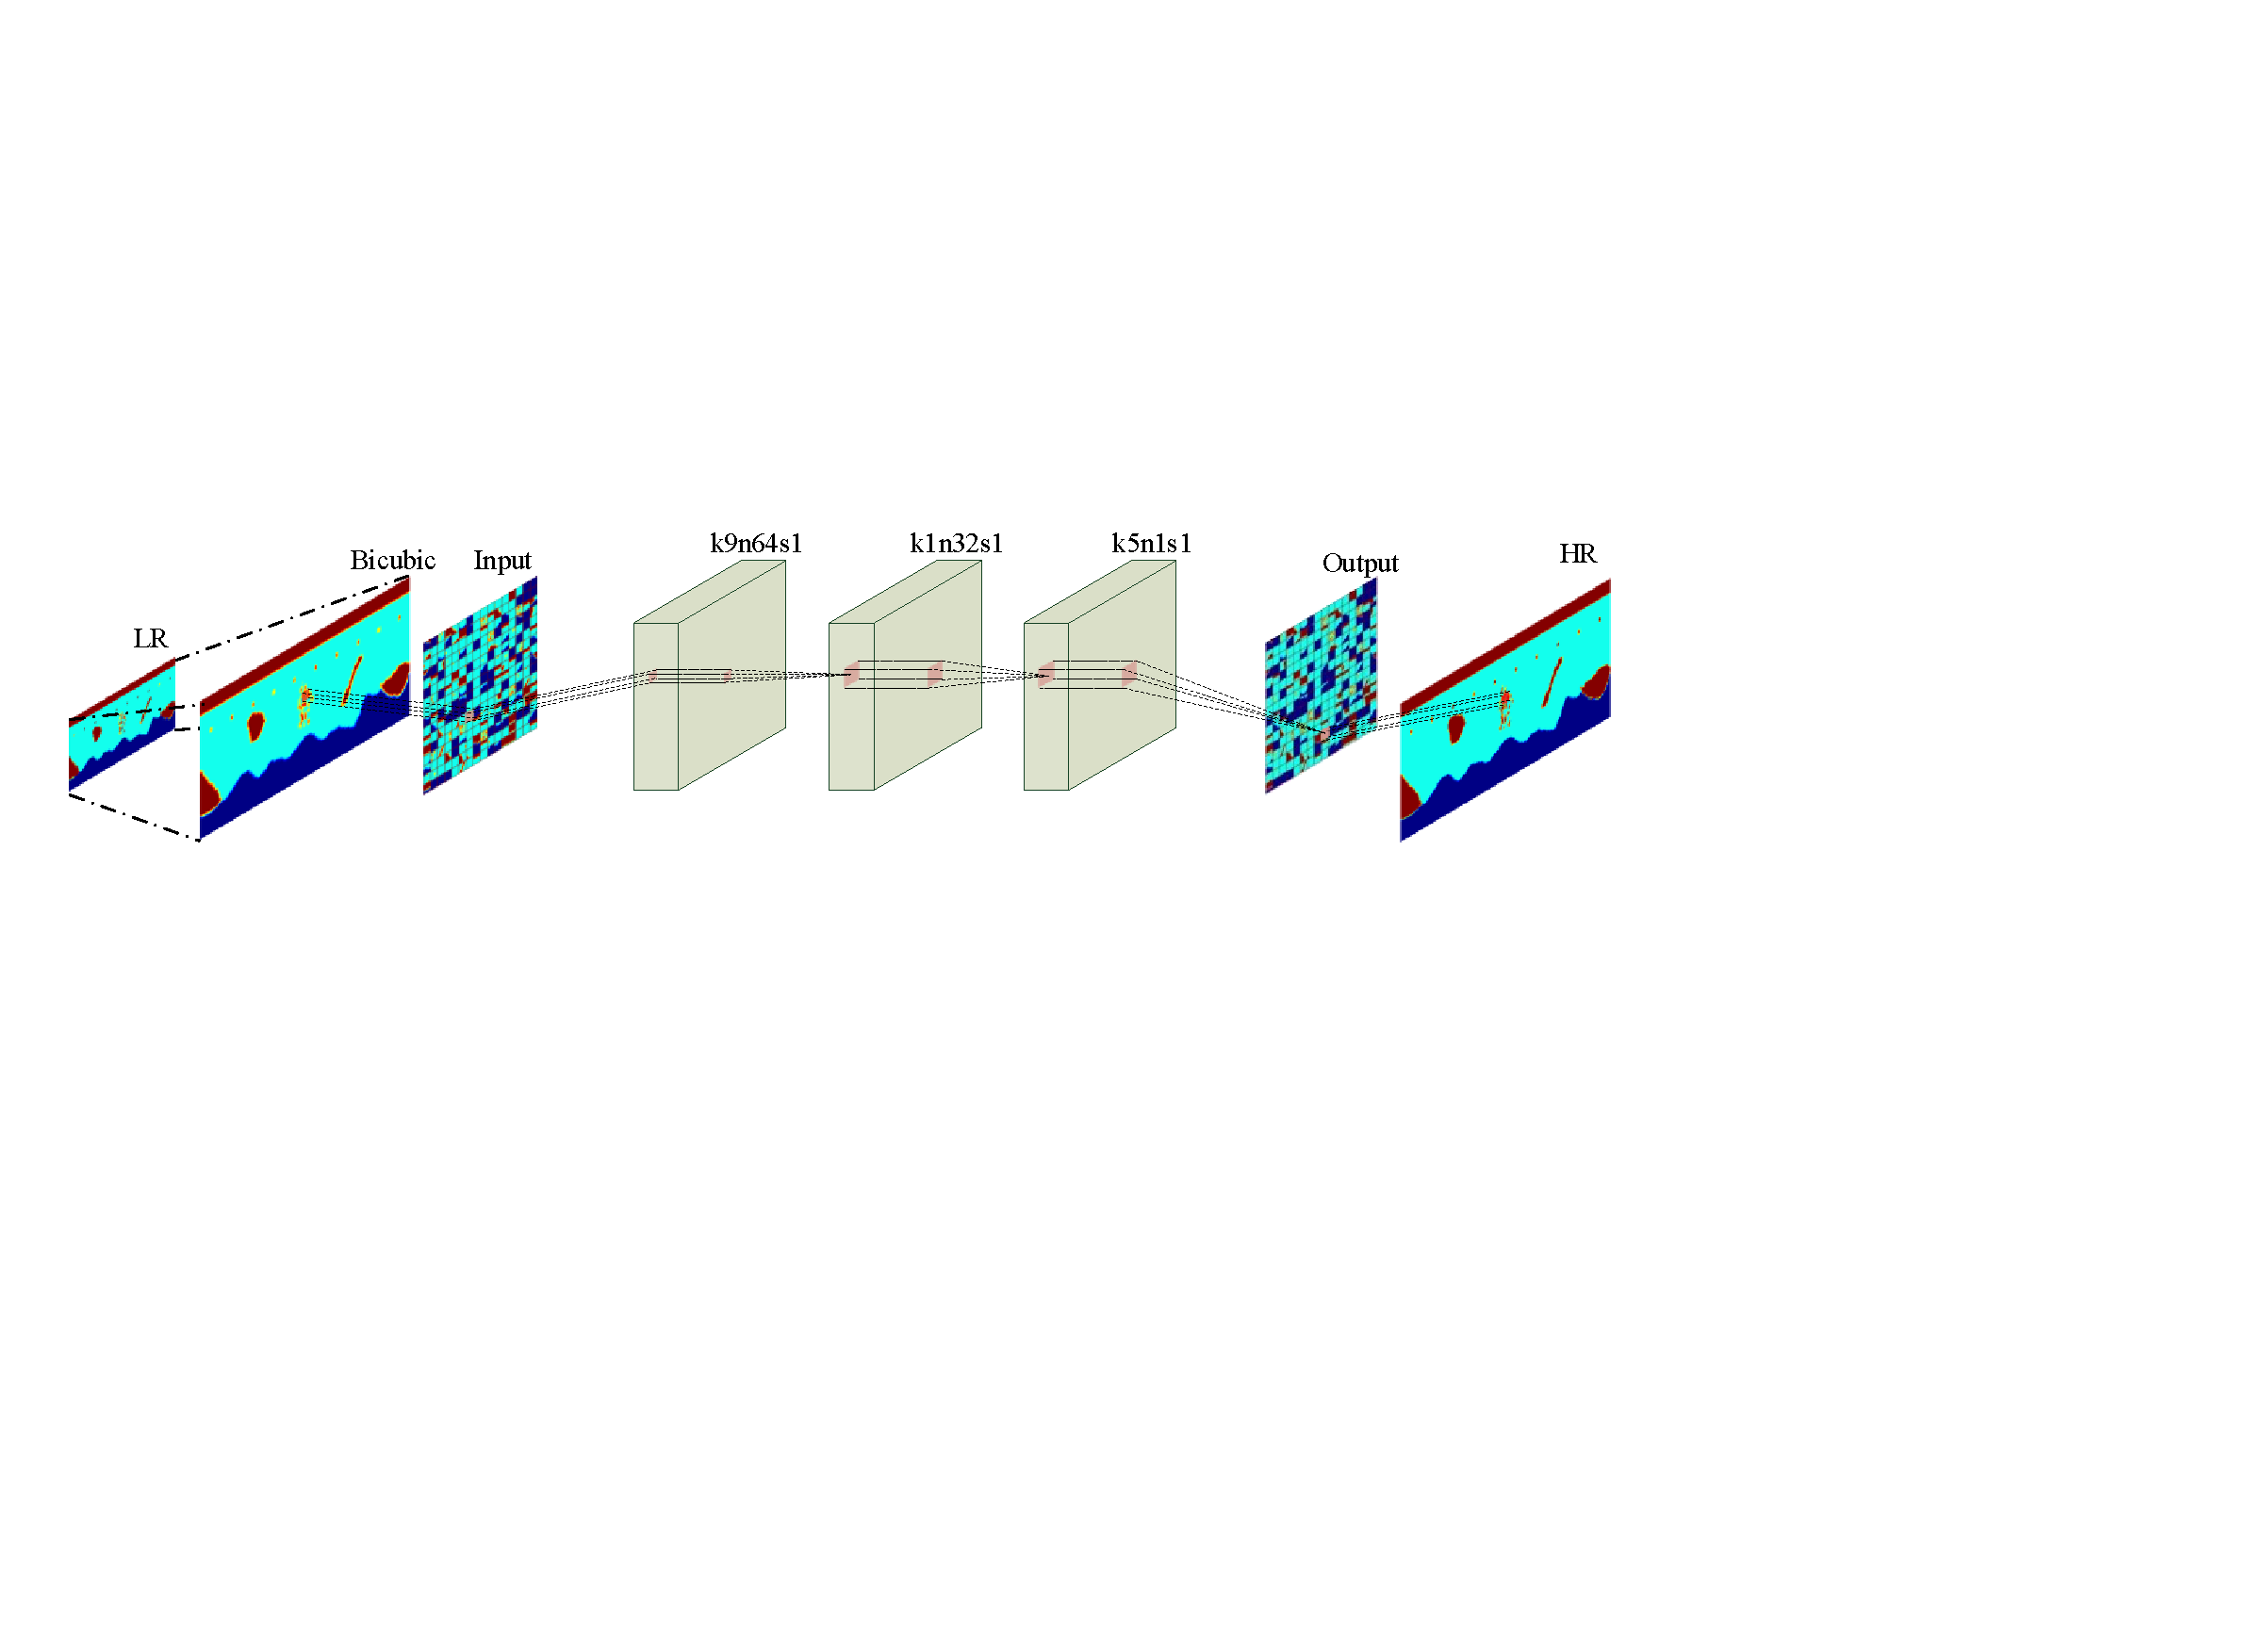
\includegraphics[width=5.5in]{./FigureFolder/Foundation/SuperResolution/SRCNN/SRCNN.pdf}
\caption{SRCNN网络结构}
\label{Fig_SRCNN}
\end{figure}
\par
图\ref{Fig_SRCNN}表示了SRCNN的全部流程,首先需要使用双三次插值算法将粗网格数据映射到细网格上,接着经过三个卷积层,得到神经网络的输出,经过不断迭代更新神经网络的权重值及偏置值,获得训练好的SRCNN网络,实现端到端的映射。使用SRCNN网络得到的细网格映射数据如图\ref{Fig_HRSRCNN}所示,此时$PSNR=28.8587dB$,从结果来看,SRCNN对于粗网格的映射处理效果要优于双三次插值方法。
\begin{figure}[htbp]
\centering
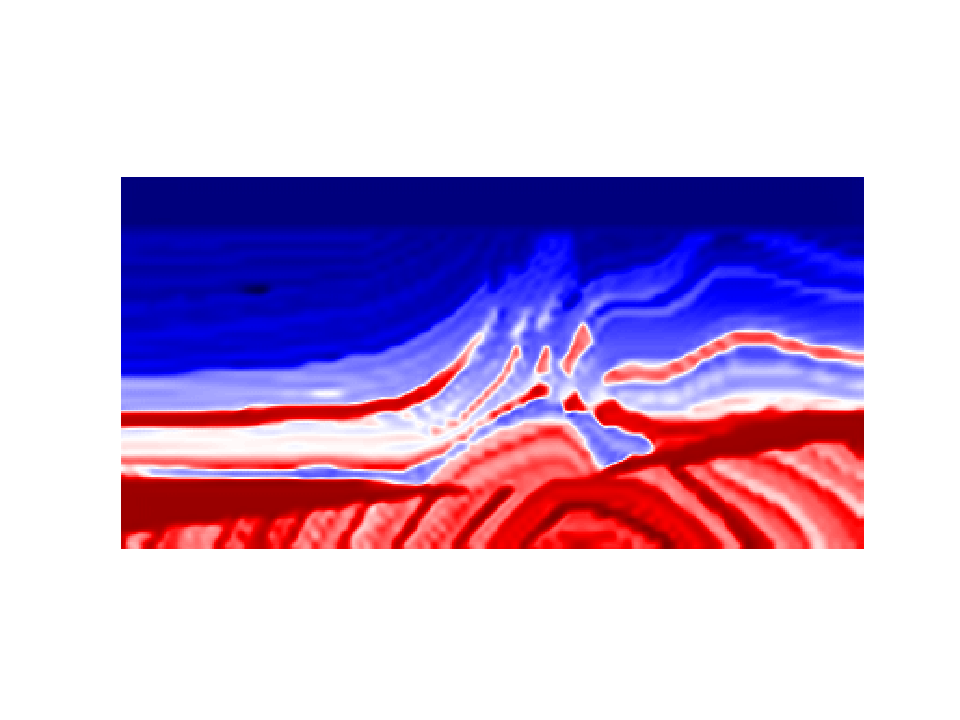
\includegraphics[width=3in]{./FigureFolder/Foundation/SuperResolution/SRCNN/HR_Marmousi.pdf}
\caption{SRCNN映射到细网格Marmousi-ii模型数据}
\label{Fig_HRSRCNN}
\end{figure}
\par
2) Efficient Sub-Pixel Convolutional Neural Network(ESPCN)的实现
\par
许多深度学习模型还结合了转置卷积进行上采样。双线性和双三次上采样是无法学习的,这意味着它只能在深度学习架构之前或之后使用,而不能在两者之间使用。可学习的上采样的其他优点是它的速度和准确性。但是,正如人们可能已经观察到的那样,采用跨步卷积梯度实现的上采样操作会增加零值以放大图像,以后必须用有意义的值填充该值。甚至更糟的是,这些零值没有可以反向传播的梯度信息。为了解决这个问题,提出了亚像素卷积神经网络层用于扩展。该层实质上使用规则的卷积层,然后使用称为相移的特定类型的图像重塑。换句话说,它们不必在像素之间放置零,而不必进行额外的计算,而是以较低的分辨率计算更多的卷积,并将生成的地图调整为放大的图像。这样,就不需要无意义的零了。使用相移的图像重塑也称为``像素混洗'',它重新排列$H \times W \times C \cdot r^2$张量的元素以形成$rH \times rW \times C$张量。ESPCN网络结构如图\ref{Fig_ESPCN}所示。
\begin{figure}[htbp]
\centering
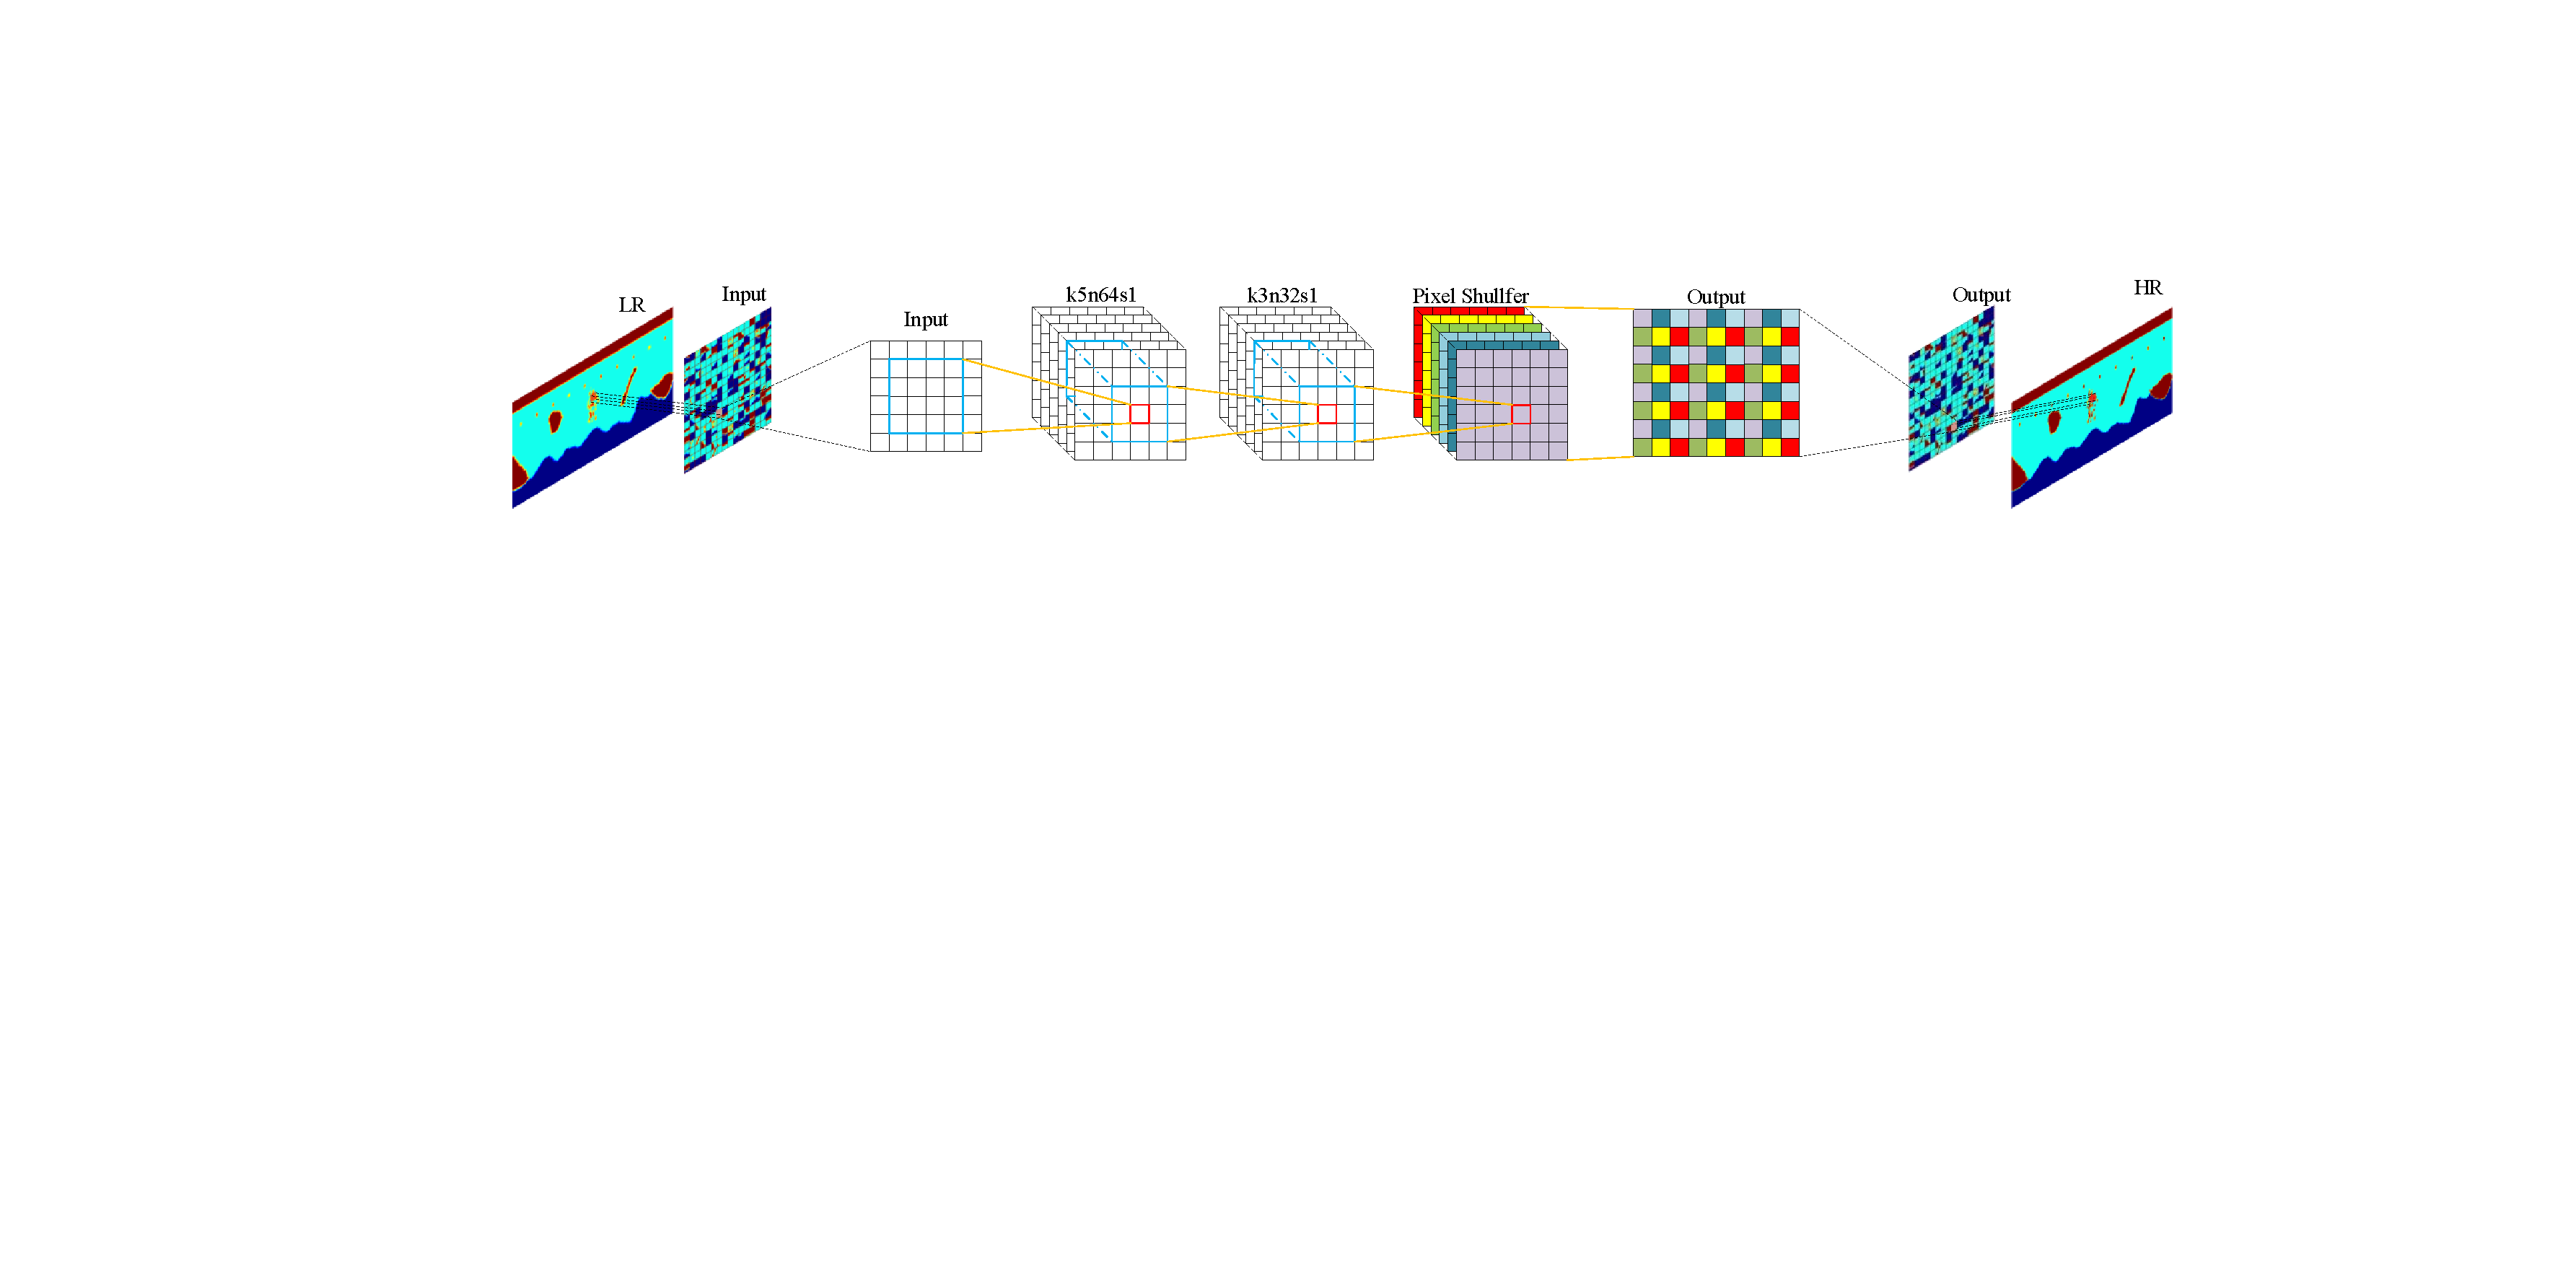
\includegraphics[width=5.5in]{./FigureFolder/Foundation/SuperResolution/ESPCN/ESPCN.pdf}
\caption{ESPCN网络结构}
\label{Fig_ESPCN}
\end{figure}
\par
图\ref{Fig_ESPCN}表示了ESPCN的全部流程,它不需要对原始数据进行处理,可以直接将低分辨率图像作为网络输入,接着经过三个卷积层,并经过一次像素混洗处理,得到神经网络的输出,经过不断迭代更新神经网络的权重值及偏置值,获得训练好的ESPCN网络,实现端到端的映射。使用ESPCN网络得到的细网格映射数据如图\ref{Fig_HRESPCN}所示,此时$PSNR=29.7388dB$,从结果来看,ESPCN不需要对原始数据进行处理,并且获得了更优的结果,不仅提高了效率,同时也提高了精度。
\begin{figure}[htbp]
\centering
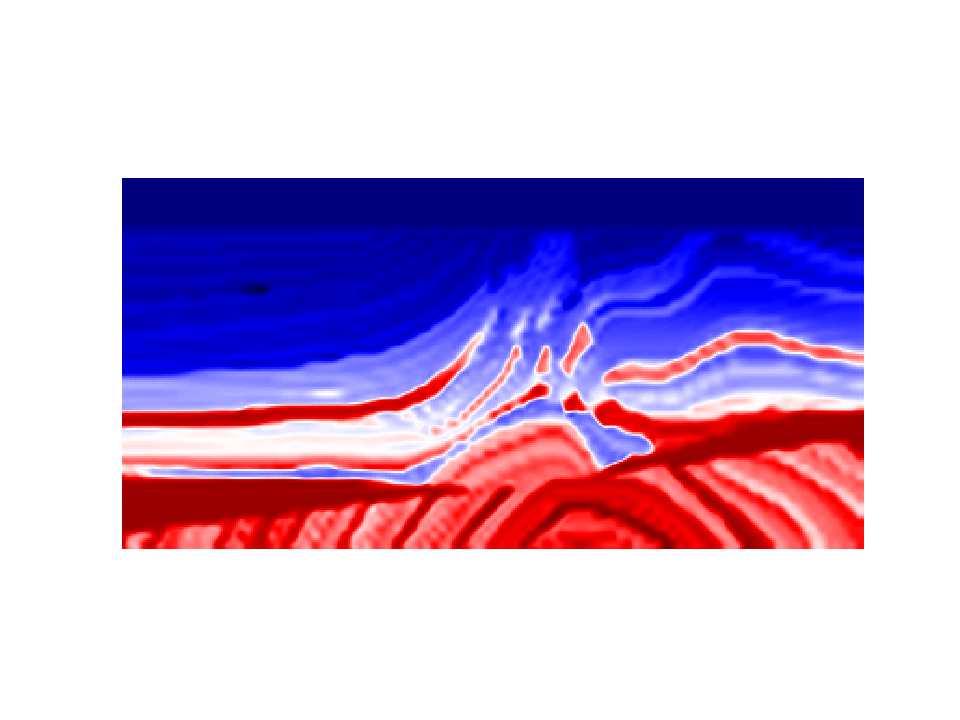
\includegraphics[width=3in]{./FigureFolder/Foundation/SuperResolution/ESPCN/HR_Marmousi.pdf}
\caption{ESPCN映射到细网格Marmousi-ii模型数据}
\label{Fig_HRESPCN}
\end{figure}
\par
3) SRGAN的实现
生成对抗网络(GANs)提供了一个强大的框架,可以生成具有高感知质量的看起来合理的自然图像。GAN程序鼓励重构物向搜索空间区域移动,从而很有可能包含照片级逼真的图像,从而更接近自然图像流形。SRGAN是一个基于GAN的网络,其中生成器(G)学习从尽可能接近HR的LR图像生成SR图像。鉴别器(D)学会将生成的SR图像与真实图像区分开。G利用ResNet和亚像素卷积进行上采样。它还将感性损失与生成性或对抗性损失相结合,以计算其损失。SRGAN网络结构如图\ref{Fig_SRGAN}所示。
\begin{figure}[htbp]
\centering
\includegraphics[width=5.5in]{./FigureFolder/Foundation/SuperResolution/GAN/SRGAN.pdf}
\caption{SRGAN网络结构}
\label{Fig_SRGAN}
\end{figure}
\par
图\ref{Fig_SRGAN}表示了SRGAN的全部流程,生成网络接受原始低分辨率数据作为输入,经过多个残差层的处理,然后经过像素混洗策略,最终得到网络的输出,将生成网络的输入作为判别器的输入,经过多个卷积层的处理,接着进入全连接层,最终输入一个判别数据真伪的概率,通过生成网络和判别网络的不断对抗学习,不断迭代更新神经网络的权重值及偏置值,获得训练好的SRGAN网络,实现端到端的映射。使用SRGAN网络得到的细网格映射数据如图\ref{Fig_HRSRGAN}所示,此时$PSNR=41.7587dB$,从结果来看,SRGAN网络相对以上技术,在精度上得到了大幅提高。
\begin{figure}[htbp]
\centering
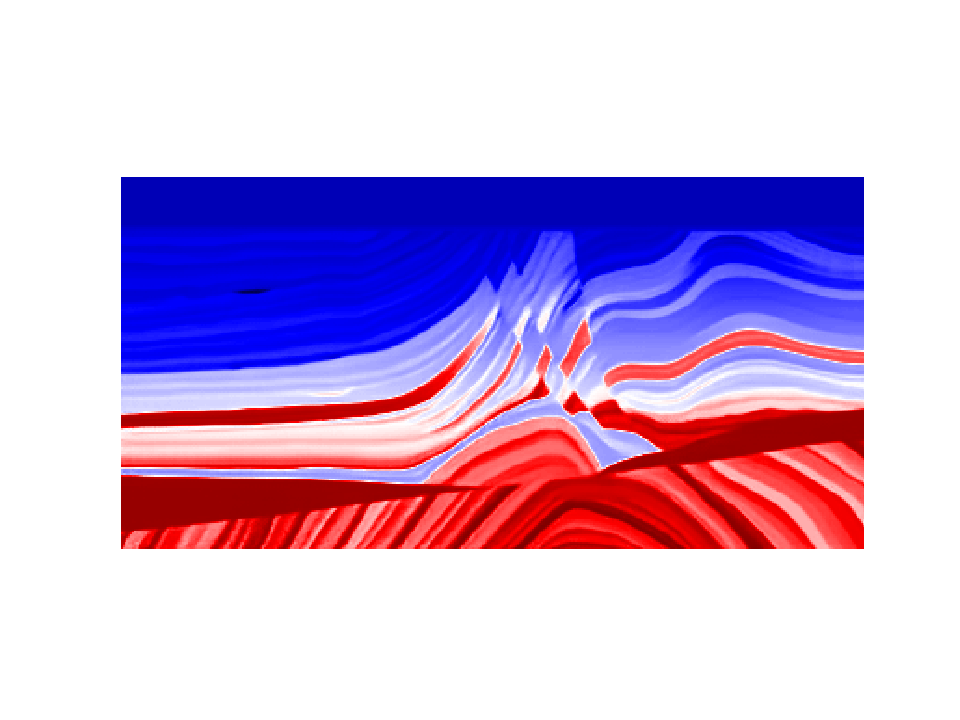
\includegraphics[width=3in]{./FigureFolder/Foundation/SuperResolution/GAN/HR_Marmousi.pdf}
\caption{SRGAN映射到细网格Marmousi-ii模型数据}
\label{Fig_HRSRGAN}
\end{figure}
\par
以上为超分辨率网格映射研究的具体进展,以上过程的详细代码及数据已发布至$https://github.com/NephilimTeam/Seismic-Super-Resolution$。
\par
\newpage
\section*{\hei\fontsize{11pt}{10pt} \selectfont \\ 七、主要参考文献}
\vskip -30pt
\bibliography{./report}
\end{document}